\documentclass[12pt]{article}\usepackage[]{graphicx}\usepackage[]{xcolor}
% maxwidth is the original width if it is less than linewidth
% otherwise use linewidth (to make sure the graphics do not exceed the margin)
\makeatletter
\def\maxwidth{ %
  \ifdim\Gin@nat@width>\linewidth
    \linewidth
  \else
    \Gin@nat@width
  \fi
}
\makeatother

\definecolor{fgcolor}{rgb}{0.345, 0.345, 0.345}
\newcommand{\hlnum}[1]{\textcolor[rgb]{0.686,0.059,0.569}{#1}}%
\newcommand{\hlstr}[1]{\textcolor[rgb]{0.192,0.494,0.8}{#1}}%
\newcommand{\hlcom}[1]{\textcolor[rgb]{0.678,0.584,0.686}{\textit{#1}}}%
\newcommand{\hlopt}[1]{\textcolor[rgb]{0,0,0}{#1}}%
\newcommand{\hlstd}[1]{\textcolor[rgb]{0.345,0.345,0.345}{#1}}%
\newcommand{\hlkwa}[1]{\textcolor[rgb]{0.161,0.373,0.58}{\textbf{#1}}}%
\newcommand{\hlkwb}[1]{\textcolor[rgb]{0.69,0.353,0.396}{#1}}%
\newcommand{\hlkwc}[1]{\textcolor[rgb]{0.333,0.667,0.333}{#1}}%
\newcommand{\hlkwd}[1]{\textcolor[rgb]{0.737,0.353,0.396}{\textbf{#1}}}%
\let\hlipl\hlkwb

\usepackage{framed}
\makeatletter
\newenvironment{kframe}{%
 \def\at@end@of@kframe{}%
 \ifinner\ifhmode%
  \def\at@end@of@kframe{\end{minipage}}%
  \begin{minipage}{\columnwidth}%
 \fi\fi%
 \def\FrameCommand##1{\hskip\@totalleftmargin \hskip-\fboxsep
 \colorbox{shadecolor}{##1}\hskip-\fboxsep
     % There is no \\@totalrightmargin, so:
     \hskip-\linewidth \hskip-\@totalleftmargin \hskip\columnwidth}%
 \MakeFramed {\advance\hsize-\width
   \@totalleftmargin\z@ \linewidth\hsize
   \@setminipage}}%
 {\par\unskip\endMakeFramed%
 \at@end@of@kframe}
\makeatother

\definecolor{shadecolor}{rgb}{.97, .97, .97}
\definecolor{messagecolor}{rgb}{0, 0, 0}
\definecolor{warningcolor}{rgb}{1, 0, 1}
\definecolor{errorcolor}{rgb}{1, 0, 0}
\newenvironment{knitrout}{}{} % an empty environment to be redefined in TeX

\usepackage{alltt}    % For submission



%% Package imports %%%%%%%%%%%%%%%%%%%%%%%%%%%%%%%%%%%%%%%%%%%

\usepackage{amsfonts}           % For access to \checkmark.
\usepackage{amsmath}            % For better symbol decorations
\usepackage{authblk}            % For a nice author block
\usepackage{booktabs}           % For nice table rules
\usepackage[official]{eurosym}  % For the euro symbol
\usepackage[figurename=Fig.]{caption} % For changing "Figure" to "Fig." in figure captions
\usepackage{chngcntr}           % To get figure and table numbering correct in the appendices
\usepackage[makeroom]{cancel}   % To show terms go to zero
\usepackage[inline]{enumitem}   % For inline enumeration
\usepackage[letterpaper, left=0.75in, right=0.75in, top=0.75in, bottom=0.75in, footskip=.25in]{geometry} % For better margins.
\usepackage[]{lineno}           % For line numbers
% \modulolinenumbers[5]
\usepackage{microtype}          % For beautiful typesetting
\usepackage{multicol}           % For multi-column layout
\usepackage{multirow}           % For multi-row layout
\usepackage{natbib}
\setlength{\bibsep}{0.0pt}      % To set the separation between entries to 0.
\usepackage{nccmath}            % For the \useshortskip command above equations
\usepackage{parcolumns}         % For multi-column layout
\usepackage{pdflscape}          % For landscape environment \begin{landscape} ... \end{landscape}
\usepackage{physics}            % For the \eval command.
\usepackage{setspace}           % For double spacing
\doublespacing
\usepackage{soul}               % For text highlighting
\usepackage[most]{tcolorbox}    % For color highlighting of text
\usepackage{tikz}               % For diagrams
\usetikzlibrary{arrows,positioning}
\usepackage{ulem}               % For strikeout command (\sout)
\usepackage{xcolor}             % For ... colors
\usepackage{xr}                 % For external references to the results paper
\externaldocument[PartII-]{HSB_results}

\usepackage{hyperref}           % hyperref should be the last package loaded


%% Macros defined by authors %%%%%%%%%%%%%%%%%%%%%%%%%%%%%%%%%

% The next command tells RStudio to do "Compile PDF" on HSB_framework.Rnw,
% instead of this file, thereby eliminating the need to switch back to HSB_framework.Rnw 
% before building the paper.
%!TEX root = ../HSB_framework.Rnw


%%%%%%%%%%%%%%%%%%%%%%%%%%%%%%%%%%%%%%%%%%%%%%%%%%%%%%%%%%%%%%
% This file contains macros for
% Heun, Semieniuk, Brockway, 
% Energy, expenditure, and consumption aspects of rebound,\\
% Part I: A rigorous analytical framework
% and
% Energy, expenditure, and consumption aspects of rebound,\\
% Part II: Applications of the framework
% 
% It is incorporated into the main file by the command
% % The next command tells RStudio to do "Compile PDF" on HSB_framework.Rnw,
% instead of this file, thereby eliminating the need to switch back to HSB_framework.Rnw 
% before building the paper.
%!TEX root = ../HSB_framework.Rnw


%%%%%%%%%%%%%%%%%%%%%%%%%%%%%%%%%%%%%%%%%%%%%%%%%%%%%%%%%%%%%%
% This file contains macros for
% Heun, Semieniuk, Brockway, 
% Energy, expenditure, and consumption aspects of rebound,\\
% Part I: A rigorous analytical framework
% and
% Energy, expenditure, and consumption aspects of rebound,\\
% Part II: Applications of the framework
% 
% It is incorporated into the main file by the command
% % The next command tells RStudio to do "Compile PDF" on HSB_framework.Rnw,
% instead of this file, thereby eliminating the need to switch back to HSB_framework.Rnw 
% before building the paper.
%!TEX root = ../HSB_framework.Rnw


%%%%%%%%%%%%%%%%%%%%%%%%%%%%%%%%%%%%%%%%%%%%%%%%%%%%%%%%%%%%%%
% This file contains macros for
% Heun, Semieniuk, Brockway, 
% Energy, expenditure, and consumption aspects of rebound,\\
% Part I: A rigorous analytical framework
% and
% Energy, expenditure, and consumption aspects of rebound,\\
% Part II: Applications of the framework
% 
% It is incorporated into the main file by the command
% \input{macros.tex}.
%%%%%%%%%%%%%%%%%%%%%%%%%%%%%%%%%%%%%%%%%%%%%%%%%%%%%%%%%%%%%%


%%%%% Override Energy Economics macros
\renewcommand{\emph}{\textit}


%%%%% Units

\newcommand{\kWhr}{kW$\cdot$hr}
\newcommand{\lmhr}{lm$\cdot$hr}
\newcommand{\passkm}{pass$\cdot$km}
\newcommand{\Whr}{W$\cdot$hr}


%%%%% Decorations for symbols

\newcommand{\rate}[1]{\dot{#1}}                    % Rate of a quantity

% Create "after" commands
\newcommand{\orig}[1]{{}{#1}^{\scriptscriptstyle \circ}}
\newcommand{\aempl}[1]{{#1}^*}
\newcommand{\asub}[1]{\hat{#1}}
\newcommand{\ainc}[1]{\bar{#1}}
\newcommand{\amacro}[1]{\tilde{#1}}

% Create the "before" commands
\newcommand{\bempl}[1]{\orig{#1}}
\newcommand{\bsub}[1]{\aempl{#1}}
\newcommand{\binc}[1]{\asub{#1}}
\newcommand{\bmacro}[1]{\ainc{#1}}

% Decoration combinations
% Rates after
\newcommand{\rorig}[1]{\orig{\rate{#1}}}
\newcommand{\raempl}[1]{\aempl{\rate{#1}}}
\newcommand{\rasub}[1]{\asub{\rate{#1}}}
\newcommand{\rainc}[1]{\ainc{\rate{#1}}}
\newcommand{\ramacro}[1]{\amacro{\rate{#1}}}

% Rates before
\newcommand{\rbempl}[1]{\rorig{#1}}
\newcommand{\rbsub}[1]{\raempl{#1}}
\newcommand{\rbinc}[1]{\rasub{#1}}
\newcommand{\rbmacro}[1]{\rainc{#1}}

%%%%% Subscript kerning

\newcommand{\om}{O\!M}
\newcommand{\omd}{O\!M\!d}
\newcommand{\md}{md}
\newcommand{\macro}{macr\!o}
\newcommand{\life}{li\!f\!e}
\newcommand{\EEU}{E\!EU}

%%%%% Expression kerning

\newcommand{\MPC}{M\!PC}


%%%%% Convenient symbols

\newcommand{\Sdot}{\rate{S}_{dev}}
\newcommand{\Mdothatprime}{\rbinc{M}^\prime}


%%%%% Elasticities and income shares

\newcommand{\eqspsUC}{\varepsilon_{\rate{q}_s\!,p_s}}
\newcommand{\eqopsUC}{\varepsilon_{\rate{q}_o\!,p_s}}
\newcommand{\eqspsC}{\varepsilon_{\rate{q}_s\!,p_s\!,c}}
\newcommand{\eqopsC}{\varepsilon_{\rate{q}_o\!,p_s\!,c}}

% originally
\newcommand{\eqspsUCorig}{\varepsilon^\circ_{\rate{q}_s\!,p_s}}
\newcommand{\eqopsUCorig}{\varepsilon^\circ_{\rate{q}_o\!,p_s}}
\newcommand{\eqspsCorig}{\varepsilon^\circ_{\rate{q}_s\!,p_s\!,c}}
\newcommand{\eqopsCorig}{\varepsilon^\circ_{\rate{q}_o\!,p_s\!,c}}
% With hats
\newcommand{\eqspsUChat}{\hat{\varepsilon}_{\rate{q}_s\!,p_s}}
\newcommand{\eqopsUChat}{\hat{\varepsilon}_{\rate{q}_o\!,p_s}}
\newcommand{\eqspsChat}{\hat{\varepsilon}_{\rate{q}_s\!,p_s\!,c}}
\newcommand{\eqopsChat}{\hat{\varepsilon}_{\rate{q}_o\!,p_s\!,c}}

\newcommand{\eqsM}{\varepsilon_{\rate{q}_s\!,\rate{M}}}
\newcommand{\eqoM}{\varepsilon_{\rate{q}_o\!,\rate{M}}}

\newcommand{\fCs}{\bempl{f}_{\rate{C}_s}}
\newcommand{\fCshat}{\asub{f}_{\rate{C}_s}}

\newcommand{\eQEpE}{\varepsilon_{\rate{Q}_E,p_E}}


%%%%% Colors

% Original spectrum colours
% \colorlet{emplcolor}{red!25!white}
% \colorlet{subcolor}{orange!25!white}
% \colorlet{inccolor}{green!25!white}
% \colorlet{macrocolor}{blue!25!white}

% New Viridis "plasma" colours
\definecolor{emplcolor}{HTML}{150789}
\definecolor{subcolor}{HTML}{99149F}
\definecolor{inccolor}{HTML}{E76F5A}
\definecolor{macrocolor}{HTML}{F7E225}



%%%%% Coloration of text background

%
% Inline color box around text
% Arguments:
%   [#1]: background color for the box
%   {#2}: text inside the box
%
\newtcbox{\inlinebox}[1][]{on line, 
colback=#1,
colframe=#1,
before upper={\rule[-2pt]{0pt}{10pt}},
boxrule=1pt,
boxsep=0pt,
left=3pt,
right=3pt,
top=2pt,
bottom=2pt}


%%%%% Colored phrases

% Emplacement effect
\newcommand{\empleffect}{\inlinebox[emplcolor]{\textcolor{white}{emplacement effect}}}
\newcommand{\empleffectadj}{\inlinebox[emplcolor]{\textcolor{white}{emplacement-effect}}}
\newcommand{\Empleffect}{\inlinebox[emplcolor]{\textcolor{white}{Emplacement effect}}}
\newcommand{\EmplEffect}{\inlinebox[emplcolor]{\textcolor{white}{Emplacement Effect}}}

% Substitution effect
\newcommand{\subeffect}{\inlinebox[subcolor]{\textcolor{white}{substitution effect}}}
\newcommand{\subeffectadj}{\inlinebox[subcolor]{\textcolor{white}{substitution-effect}}}
\newcommand{\Subeffect}{\inlinebox[subcolor]{\textcolor{white}{Substitution effect}}}
\newcommand{\SubEffect}{\inlinebox[subcolor]{\textcolor{white}{Substitution Effect}}}

% Income effect
\newcommand{\inceffect}{\inlinebox[inccolor]{\textcolor{black}{income effect}}}
\newcommand{\inceffectadj}{\inlinebox[inccolor]{\textcolor{black}{income-effect}}}
\newcommand{\Inceffect}{\inlinebox[inccolor]{\textcolor{black}{Income effect}}}
\newcommand{\IncEffect}{\inlinebox[inccolor]{\textcolor{black}{Income Effect}}}

% Macro effect
\newcommand{\macroeffect}{\inlinebox[macrocolor]{\textcolor{black}{macro effect}}}
\newcommand{\macroeffectadj}{\inlinebox[macrocolor]{\textcolor{black}{macro-effect}}}
\newcommand{\Macroeffect}{\inlinebox[macrocolor]{\textcolor{black}{Macro effect}}}
\newcommand{\MacroEffect}{\inlinebox[macrocolor]{\textcolor{black}{Macro Effect}}}


%%%%% minipage for assumptions and constraints tables
% Arguments:
%   #1: Width (multiple of \linewidth
%   #2: text inside the minipage
%
\newcommand{\mptable}[2]{\begin{minipage}{#1\linewidth} \useshortskip{} \begin{equation} #2 \end{equation} \end{minipage}}


%%%%% Oft-used references

\newcommand{\Ba}[1]{\citeauthor[#1]{Borenstein:2015aa}}
\newcommand{\Bapp}[1]{\citeauthor[#1]{Borenstein:2015aa}'s \citeyearpar{Borenstein:2015aa}}
\newcommand{\Bp}[1]{\citep[#1]{Borenstein:2015aa}}
\newcommand{\Bt}[1]{\citet[#1]{Borenstein:2015aa}}

\newcommand{\Ta}[1]{\citeauthor[#1]{Thomas:2013aa}}
\newcommand{\Tapp}[1]{\citeauthor[#1]{Thomas:2013aa}'s \citeyearpar{Thomas:2013aa}}
\newcommand{\Tp}[1]{\citep[#1]{Thomas:2013aa, Thomas:2013ab}}
\newcommand{\Tpone}[1]{\citep[#1]{Thomas:2013aa}}
\newcommand{\Tptwo}[1]{\citep[#1]{Thomas:2013ab}}
\newcommand{\Tt}[1]{\citet[#1]{Thomas:2013aa, Thomas:2013ab}}
\newcommand{\Ttone}[1]{\citet[#1]{Thomas:2013aa}}
\newcommand{\Tttwo}[1]{\citet[#1]{Thomas:2013ab}}


%%%%% Derivation pages

% Column widths
\newcommand{\derivtextsize}{\footnotesize}
\newcommand{\derivpageleftcolwidth}{0.11\textwidth}
\newcommand{\derivpageenergycolwidth}{0.6\textwidth}
\newcommand{\derivpagefinancialcolwidth}{0.6\textwidth}

% Horizontal rule between sections of derivations

\newcommand{\sectionsep}{\noindent\rule{1.4\textwidth}{0.4pt}}


%
% Derivation section
% Arguments:
%   #1: accounting stage (original, prime, etc.)
%   #2: energy column
%   #3: financial column
%
\newcommand{\derivsection}[3]{%

\derivtextsize{}

\begin{minipage}[t]{\derivpageleftcolwidth}
~\\#1
\end{minipage}
%
%
%
\begin{minipage}[t]{\derivpageenergycolwidth}
#2
\end{minipage}
%
~
%
\begin{minipage}[t]{\derivpagefinancialcolwidth}
#3
\end{minipage}

\normalsize{}

}


%
% Derivation page header
% Arguments:
%   #1: Effect type header text (e.g., Emplacement Effect)
%
\newcommand{\derivheader}[1]{

\begin{center}
  #1
\end{center}

\derivsection{}
{\begin{center}\emph{Energy analysis}\end{center}}
{\begin{center}\emph{Financial analysis}\end{center}}

}


% Equations

% Efficiency ratios
\newcommand{\etaratioinline}{\amacro{\eta}/\bempl{\eta}}
\newcommand{\etaratiostacked}{\frac{\amacro{\eta}}{\bempl{\eta}}}

% Derivative with respect to efficiency ratio
\newcommand{\dbydetaeta}{\frac{\mathrm{d}}{\mathrm{d}(\etaratioinline{})}}


% Original
\newcommand{\Eacctorig}{\rbempl{E} = \rbempl{E}_s + \rbempl{E}_{emb} + (\rbempl{C}_{\omd} + \rbempl{C}_o) I_E}
\newcommand{\Macctorig}{\rate{M} = p_E \rbempl{E}_s + \bempl{R}_\alpha \rbempl{C}_{cap} + \rbempl{C}_{\omd} + \rbempl{C}_o + \rbempl{N}}

% Before emplacement effect (same as original)
\newcommand{\Eacctbempl}{\Eacctorig}      
\newcommand{\Macctbempl}{\Macctorig}      

% After emplacement effect
\newcommand{\Eacctaempl}{\raempl{E} = \raempl{E}_s + \raempl{E}_{emb} + (\raempl{C}_{\omd} + \raempl{C}_o) I_E}                  
\newcommand{\Macctaempl}{\rate{M} = p_E \raempl{E}_s + \aempl{R}_\alpha \raempl{C}_{cap} + \raempl{C}_{\omd} + \raempl{C}_o + \raempl{N}}         

% Before substitution effect (same as after emplacement effect)
\newcommand{\Eacctbsub}{\Eacctaempl}
\newcommand{\Macctbsub}{\Macctaempl}

% After substitution effect
\newcommand{\Eacctasub}{\rasub{E} = \rasub{E}_s + \rasub{E}_{emb} + (\rasub{C}_{\omd} + \rasub{C}_o) I_E}
\newcommand{\Macctasub}{\rate{M} = p_E \rasub{E}_s + \asub{R}_\alpha \rasub{C}_{cap} + \rasub{C}_{\omd} + \rasub{C}_o + \rasub{N}}

% Before income effect (same as after substitution effect)
\newcommand{\Eacctbinc}{\Eacctasub}
\newcommand{\Macctbinc}{\Macctasub}

% After income effect
\newcommand{\Eacctainc}{\rainc{E} = \rainc{E}_s + \rainc{E}_{emb} + (\rainc{C}_{\omd} + \rainc{C}_o) I_E}
\newcommand{\Macctainc}{\rate{M} = p_E \rainc{E}_s + \ainc{R}_\alpha \rainc{C}_{cap} + \rainc{C}_{\omd} + \rainc{C}_o + \rainc{N}}

% Embodied energy rebound
\newcommand{\Reembeqn}{\frac{\left( \frac{\aempl{E}_{emb}}{\bempl{E}_{emb}}
  \frac{\bempl{t}_{\life}}{\aempl{t}_{\life}} - 1 \right) \rbempl{E}_{emb}}{\Sdot}}
  
% Ops, Maintenance, and disposal energy rebound
\newcommand{\ReOMdeqn}{\frac{\left( \frac{\raempl{C}_{\omd}}{\rbempl{C}_{\omd}} - 1 \right) \rbempl{C}_{\omd} I_E}{\Sdot}}

% Equation for S_dot_dev
% \newcommand{\Sdoteqn}{\left( \etaratiostacked - 1 \right)\!\etaratiostacked \rbempl{E}_s}
\newcommand{\Sdoteqn}{\left( \etaratiostacked - 1 \right)\! 
                            \frac{\bempl{\eta}}{\amacro{\eta}} \rbempl{E}_s}

% Equation for Re_dsub
\newcommand{\Redsubeqn}{\frac{\left( \etaratiostacked \right)^{-\eqspsUC} - 1}
                        {\etaratiostacked - 1}}
                        
% Equation for Re_isub
\newcommand{\Reisubeqn}{\frac{{\left( \etaratiostacked  \right)}
                          ^{-\eqopsC} - 1}{\etaratiostacked - 1} \; 
                          \etaratiostacked \; 
                          \frac{\rbempl{C}_o I_E}{\rbempl{E}_s}}
                          
% CES utility equation
\newcommand{\cesutility}{\left[ \fCs \left( \frac{\rate{q}_s}{\rbempl{q}_s} \right)^\rho 
        + (1-\fCs) \left( \frac{\rate{C}_o}{\rbempl{C}_o} \right)^\rho  \right]^{(1/\rho)}}
        
% Equation for q_s_hat/q_s_orig
\newcommand{\qssolution}{\left\{ \fCs + (1-\fCs)
      \left[ \left(  \frac{1-\fCs}{\fCs}  \right) \frac{\amacro{p}_s \rbempl{q}_s}{\rbempl{C}_o}  \right]
                                                  ^{\rho / (1 - \rho)} \right\} ^ {-1/\rho}}

% Equation for C_o_hat/C_o_orig
\newcommand{\Cosolution}{ \left( 1 + \fCs \left\{ \left[ \left( \frac{1-\fCs}{\fCs} \right)
          \frac{\amacro{p}_s \rbempl{q}_s}{\rbempl{C}_o} \right] ^{\rho/(\rho - 1)} - 1 \right\} \right)^{-1/\rho}}

% Equation for Re_dsub for the CES utility model
\newcommand{\RedsubCES}{\frac{\qssolution{} - 1}{\etaratiostacked{} - 1}}

% Equation for Re_isub for the CES utility model
\newcommand{\ReisubCES}{\frac{\Cosolution{} - 1}{\etaratiostacked{} - 1}
                         \etaratiostacked \; 
                          \frac{\rbempl{C}_o I_E}{\rbempl{E}_s}}


% Equation for Re_dinc, approximate method
\newcommand{\Redinceqnapprox}{\frac{ \left( 1 + \frac{\rbinc{N}}{\Mdothatprime} \right) ^{\eqsM} - 1}
              { \etaratiostacked - 1 } \left( \etaratiostacked \right)^{-\eqspsC}}

% Equation for Re_dinc, exact method
\newcommand{\Redinceqnexact}{\frac{ \left( 1 + \frac{\rbinc{N}}{\Mdothatprime} \right) ^{\eqsM} - 1}
              { \etaratiostacked - 1 } \qssolution{} }

% Equation for Re_cap
\newcommand{\Recapeqn}{\frac{\Delta \aempl{(R_\alpha \rate{C}_{cap})} I_E}{\Sdot}}

% Equation for Re_iinc, approximate method
\newcommand{\Reiinceqnapprox}{\frac{\left( 1 + \frac{\rbinc{N}}{\Mdothatprime} \right)^{\eqoM} - 1}{\etaratiostacked - 1} 
              \left( \etaratiostacked \right)^{1 - \eqopsC}
              \frac{\rbempl{C}_o I_E}{\rbempl{E}_s}}

% Equation for Re_iinc, exact method
% \newcommand{\Reiinceqnexact}{\frac{\left( 1 + \frac{\rbinc{N}}{\Mdothatprime} \right)^{\eqoM} - 1}{\etaratiostacked - 1} 
%               \left( \etaratiostacked \right)
%               \left( \frac{\rasub{C}_o}{\rorig{C}_o} \right) 
%               \frac{\rbempl{C}_o I_E}{\rbempl{E}_s}}

\newcommand{\Reiinceqnexact}{\frac{\left( 1 + \frac{\rbinc{N}}{\Mdothatprime} \right)^{\eqoM} - 1}{\etaratiostacked - 1} 
              \left( \etaratiostacked \right)
              \frac{\rbempl{C}_o I_E}{\rbempl{E}_s}
              \Cosolution{}}



% Equation for Re_d (total direct rebound)
\newcommand{\Redeqn}{\frac{ \left( \etaratiostacked \right)^{-\eqspsC}
             \left( 1 + \frac{\rasub{N}}{\rbempl{M}} \right)^{\eqsM}   - 1}
         {\etaratiostacked - 1}}

% Equation for Re_macro
% \newcommand{\Remacroeqn}{k (p_E I_E - Re_{cap} - Re_{\md} - p_E I_E Re_{dsub} - Re_{isub})}
\newcommand{\Remacroeqn}{k (p_E I_E - Re_{cap} - Re_{\omd})}

% Equation for Re_tot
% \newcommand{\Retoteqn}{&Re_{emb} - k Re_{cap} + (1-k) Re_{\md}         \nonumber \\
%                        &+ (1 - k p_E I_E) Re_{dsub} + (1 - k) Re_{isub}   \nonumber \\
%                        &+ Re_{dinc} + Re_{iinc} +  k p_E I_E}
% \newcommand{\Retoteqn}{&Re_{emb} + k (p_E I_E - Re_{cap}) + (1-k) Re_{\md}   \nonumber \\
%                        &+ Re_{dsub} + Re_{isub}                              \nonumber \\
%                        &+ Re_{dinc} + Re_{iinc}}
\newcommand{\Retoteqn}{Re_{emb} + k (p_E I_E - Re_{cap}) + (1-k) Re_{\omd} + Re_{dsub} + Re_{isub} + Re_{dinc} + Re_{iinc}}
                 

%%%% Income preference equations

% Equation for energy service income preferences
\newcommand{\incprefseqn}{\frac{\rainc{q}_s}{\rbinc{q}_s} = \left( 1 + \frac{\rbinc{N}}{\Mdothatprime}  \right) ^{\eqsM}}

% Equation for other goods income preferences
\newcommand{\incprefoeqn}{\frac{\rainc{q}_o}{\rbinc{q}_o} = \left( 1 + \frac{\rbinc{N}}{\Mdothatprime}  \right) ^{\eqoM}}

% Equation for effective income
% \newcommand{\effinceqn}{\Mdothatprime \equiv \rbempl{M} - \rbempl{C}_{cap} - \rbempl{C}_{\md} 
%                         - \rate{G} + p_E \Delta \rbinc{E}_s + \Delta \rbinc{C}_o}
\newcommand{\effinceqn}{\Mdothatprime \equiv \rate{M} - \aempl{R}_\alpha \raempl{C}_{cap} - \raempl{C}_{\omd} - \rasub{N}}


%%%% Budget constraint symbols and equation

\newcommand{\tlife}{t_{li\!f\!e}}
\newcommand{\oneyr}{1\,\mathrm{yr}}
\newcommand{\twoyr}{2\,\mathrm{yr}}
\newcommand{\itlife}{i\,t_{li\!f\!e}}
\newcommand{\iyr}{i\,\mathrm{yr}}

\newcommand{\budgetconstraint}{\rate{M} - \orig{R}_\alpha \rorig{C}_{cap} - \rorig{C}_{\omd} = \orig{p}_E \frac{\rorig{q}_s}{\orig{\eta}} + p_o \rorig{q}_o}


%%%% Proof characters
% Equal sign with question mark above
\DeclareRobustCommand{\questionequal}{\stackrel{?}{=}}




% Segments and lines
% Arguments:
%   #1: left character
%   #2: line color
%   #3: line thickness (e.g., 0.1 mm)
%   #4: right character
% Note that \raisebox{0.9 mm} moves the line up from the baseline.
% Also, \line(1,0){12} gives a horizontal line with length "12" (unknown units!)
% (1, 0) is the slope (1 unit to right, 0 units up).
\newcommand{\seg}[4]{#1\linethickness{#3}\raisebox{0.88 mm}{\textcolor{#2}{\line(1,0){12}}}#4}

% Construction lines
\newcommand{\iicirc}{\seg{$\bempl{\text{i}}$}{black}{0.3 mm}{$\,\bempl{\text{i}}$}}
\newcommand{\iibar}{\seg{$\bmacro{\text{i}}$}{black}{0.3 mm}{$\,\bmacro{\text{i}}$}}
\newcommand{\rr}{\seg{r}{black}{0.1 mm}{r}}
\newcommand{\circcirc}{\seg{$\circ$}{black}{0.1 mm}{$\circ$}}
\newcommand{\starstar}{\seg{$*$}{black}{0.1 mm}{$*$}}
\newcommand{\hathat}{\seg{$\wedge$}{black}{0.1 mm}{$\wedge$}}
\newcommand{\barbar}{\seg{$-\,$}{black}{0.1 mm}{$\, -$}}

% Line segments
\newcommand{\circa}{\seg{$\circ$}{emplcolor}{0.6 mm}{$a$}}
% \newcommand{\ab}{\seg{a}{emplcolor}{0.6 mm}{b}}
\newcommand{\ab}{$a$\tikz[baseline=-0.6ex]\draw [line width=0.6mm,dotted,emplcolor] (0,0) -- (0.45,0);$b$}
\newcommand{\bstar}{\seg{$b\,$}{emplcolor}{0.6 mm}{$*$}}
\newcommand{\starc}{\seg{$*$}{subcolor}{0.6 mm}{$\,c$}}
\newcommand{\chat}{\seg{$c\,$}{subcolor}{0.6 mm}{$\wedge$}}
\newcommand{\hatd}{\seg{$\wedge$}{inccolor}{0.6 mm}{$\,d$}}
\newcommand{\dbar}{\seg{$d$}{inccolor}{0.6 mm}{$\,-$}}
\newcommand{\hatbar}{\seg{$\wedge$}{inccolor}{0.6 mm}{$\,-$}}
\newcommand{\bartilde}{\seg{$- \,$}{macrocolor}{0.6 mm}{$\, \sim$}}


% Rotated text for tables
% See
% https://tex.stackexchange.com/questions/98388/how-to-make-table-with-rotated-table-headers-in-latex/98439#98439
% for details.
\newcommand{\rot}{\rotatebox{90}}


% A "rating" command for filled circles with tikz.
% See 
% https://tex.stackexchange.com/questions/194955/get-partly-filled-circle-symbol-scale-linearly-with-parameter
% for details.
\newcommand{\rating}[2][0.75ex]{%
  \pgfmathsetmacro\th{asin(#2/50-1)}% (theta angle of polar coordinates)
    \tikz{%
      \fill[black] (\th:#1) arc (\th:-180-\th:#1) -- cycle;
      \draw[black, thin, radius=#1] (0,0) circle;
    }%
}.
%%%%%%%%%%%%%%%%%%%%%%%%%%%%%%%%%%%%%%%%%%%%%%%%%%%%%%%%%%%%%%


%%%%% Override Energy Economics macros
\renewcommand{\emph}{\textit}


%%%%% Units

\newcommand{\kWhr}{kW$\cdot$hr}
\newcommand{\lmhr}{lm$\cdot$hr}
\newcommand{\passkm}{pass$\cdot$km}
\newcommand{\Whr}{W$\cdot$hr}


%%%%% Decorations for symbols

\newcommand{\rate}[1]{\dot{#1}}                    % Rate of a quantity

% Create "after" commands
\newcommand{\orig}[1]{{}{#1}^{\scriptscriptstyle \circ}}
\newcommand{\aempl}[1]{{#1}^*}
\newcommand{\asub}[1]{\hat{#1}}
\newcommand{\ainc}[1]{\bar{#1}}
\newcommand{\amacro}[1]{\tilde{#1}}

% Create the "before" commands
\newcommand{\bempl}[1]{\orig{#1}}
\newcommand{\bsub}[1]{\aempl{#1}}
\newcommand{\binc}[1]{\asub{#1}}
\newcommand{\bmacro}[1]{\ainc{#1}}

% Decoration combinations
% Rates after
\newcommand{\rorig}[1]{\orig{\rate{#1}}}
\newcommand{\raempl}[1]{\aempl{\rate{#1}}}
\newcommand{\rasub}[1]{\asub{\rate{#1}}}
\newcommand{\rainc}[1]{\ainc{\rate{#1}}}
\newcommand{\ramacro}[1]{\amacro{\rate{#1}}}

% Rates before
\newcommand{\rbempl}[1]{\rorig{#1}}
\newcommand{\rbsub}[1]{\raempl{#1}}
\newcommand{\rbinc}[1]{\rasub{#1}}
\newcommand{\rbmacro}[1]{\rainc{#1}}

%%%%% Subscript kerning

\newcommand{\om}{O\!M}
\newcommand{\omd}{O\!M\!d}
\newcommand{\md}{md}
\newcommand{\macro}{macr\!o}
\newcommand{\life}{li\!f\!e}
\newcommand{\EEU}{E\!EU}

%%%%% Expression kerning

\newcommand{\MPC}{M\!PC}


%%%%% Convenient symbols

\newcommand{\Sdot}{\rate{S}_{dev}}
\newcommand{\Mdothatprime}{\rbinc{M}^\prime}


%%%%% Elasticities and income shares

\newcommand{\eqspsUC}{\varepsilon_{\rate{q}_s\!,p_s}}
\newcommand{\eqopsUC}{\varepsilon_{\rate{q}_o\!,p_s}}
\newcommand{\eqspsC}{\varepsilon_{\rate{q}_s\!,p_s\!,c}}
\newcommand{\eqopsC}{\varepsilon_{\rate{q}_o\!,p_s\!,c}}

% originally
\newcommand{\eqspsUCorig}{\varepsilon^\circ_{\rate{q}_s\!,p_s}}
\newcommand{\eqopsUCorig}{\varepsilon^\circ_{\rate{q}_o\!,p_s}}
\newcommand{\eqspsCorig}{\varepsilon^\circ_{\rate{q}_s\!,p_s\!,c}}
\newcommand{\eqopsCorig}{\varepsilon^\circ_{\rate{q}_o\!,p_s\!,c}}
% With hats
\newcommand{\eqspsUChat}{\hat{\varepsilon}_{\rate{q}_s\!,p_s}}
\newcommand{\eqopsUChat}{\hat{\varepsilon}_{\rate{q}_o\!,p_s}}
\newcommand{\eqspsChat}{\hat{\varepsilon}_{\rate{q}_s\!,p_s\!,c}}
\newcommand{\eqopsChat}{\hat{\varepsilon}_{\rate{q}_o\!,p_s\!,c}}

\newcommand{\eqsM}{\varepsilon_{\rate{q}_s\!,\rate{M}}}
\newcommand{\eqoM}{\varepsilon_{\rate{q}_o\!,\rate{M}}}

\newcommand{\fCs}{\bempl{f}_{\rate{C}_s}}
\newcommand{\fCshat}{\asub{f}_{\rate{C}_s}}

\newcommand{\eQEpE}{\varepsilon_{\rate{Q}_E,p_E}}


%%%%% Colors

% Original spectrum colours
% \colorlet{emplcolor}{red!25!white}
% \colorlet{subcolor}{orange!25!white}
% \colorlet{inccolor}{green!25!white}
% \colorlet{macrocolor}{blue!25!white}

% New Viridis "plasma" colours
\definecolor{emplcolor}{HTML}{150789}
\definecolor{subcolor}{HTML}{99149F}
\definecolor{inccolor}{HTML}{E76F5A}
\definecolor{macrocolor}{HTML}{F7E225}



%%%%% Coloration of text background

%
% Inline color box around text
% Arguments:
%   [#1]: background color for the box
%   {#2}: text inside the box
%
\newtcbox{\inlinebox}[1][]{on line, 
colback=#1,
colframe=#1,
before upper={\rule[-2pt]{0pt}{10pt}},
boxrule=1pt,
boxsep=0pt,
left=3pt,
right=3pt,
top=2pt,
bottom=2pt}


%%%%% Colored phrases

% Emplacement effect
\newcommand{\empleffect}{\inlinebox[emplcolor]{\textcolor{white}{emplacement effect}}}
\newcommand{\empleffectadj}{\inlinebox[emplcolor]{\textcolor{white}{emplacement-effect}}}
\newcommand{\Empleffect}{\inlinebox[emplcolor]{\textcolor{white}{Emplacement effect}}}
\newcommand{\EmplEffect}{\inlinebox[emplcolor]{\textcolor{white}{Emplacement Effect}}}

% Substitution effect
\newcommand{\subeffect}{\inlinebox[subcolor]{\textcolor{white}{substitution effect}}}
\newcommand{\subeffectadj}{\inlinebox[subcolor]{\textcolor{white}{substitution-effect}}}
\newcommand{\Subeffect}{\inlinebox[subcolor]{\textcolor{white}{Substitution effect}}}
\newcommand{\SubEffect}{\inlinebox[subcolor]{\textcolor{white}{Substitution Effect}}}

% Income effect
\newcommand{\inceffect}{\inlinebox[inccolor]{\textcolor{black}{income effect}}}
\newcommand{\inceffectadj}{\inlinebox[inccolor]{\textcolor{black}{income-effect}}}
\newcommand{\Inceffect}{\inlinebox[inccolor]{\textcolor{black}{Income effect}}}
\newcommand{\IncEffect}{\inlinebox[inccolor]{\textcolor{black}{Income Effect}}}

% Macro effect
\newcommand{\macroeffect}{\inlinebox[macrocolor]{\textcolor{black}{macro effect}}}
\newcommand{\macroeffectadj}{\inlinebox[macrocolor]{\textcolor{black}{macro-effect}}}
\newcommand{\Macroeffect}{\inlinebox[macrocolor]{\textcolor{black}{Macro effect}}}
\newcommand{\MacroEffect}{\inlinebox[macrocolor]{\textcolor{black}{Macro Effect}}}


%%%%% minipage for assumptions and constraints tables
% Arguments:
%   #1: Width (multiple of \linewidth
%   #2: text inside the minipage
%
\newcommand{\mptable}[2]{\begin{minipage}{#1\linewidth} \useshortskip{} \begin{equation} #2 \end{equation} \end{minipage}}


%%%%% Oft-used references

\newcommand{\Ba}[1]{\citeauthor[#1]{Borenstein:2015aa}}
\newcommand{\Bapp}[1]{\citeauthor[#1]{Borenstein:2015aa}'s \citeyearpar{Borenstein:2015aa}}
\newcommand{\Bp}[1]{\citep[#1]{Borenstein:2015aa}}
\newcommand{\Bt}[1]{\citet[#1]{Borenstein:2015aa}}

\newcommand{\Ta}[1]{\citeauthor[#1]{Thomas:2013aa}}
\newcommand{\Tapp}[1]{\citeauthor[#1]{Thomas:2013aa}'s \citeyearpar{Thomas:2013aa}}
\newcommand{\Tp}[1]{\citep[#1]{Thomas:2013aa, Thomas:2013ab}}
\newcommand{\Tpone}[1]{\citep[#1]{Thomas:2013aa}}
\newcommand{\Tptwo}[1]{\citep[#1]{Thomas:2013ab}}
\newcommand{\Tt}[1]{\citet[#1]{Thomas:2013aa, Thomas:2013ab}}
\newcommand{\Ttone}[1]{\citet[#1]{Thomas:2013aa}}
\newcommand{\Tttwo}[1]{\citet[#1]{Thomas:2013ab}}


%%%%% Derivation pages

% Column widths
\newcommand{\derivtextsize}{\footnotesize}
\newcommand{\derivpageleftcolwidth}{0.11\textwidth}
\newcommand{\derivpageenergycolwidth}{0.6\textwidth}
\newcommand{\derivpagefinancialcolwidth}{0.6\textwidth}

% Horizontal rule between sections of derivations

\newcommand{\sectionsep}{\noindent\rule{1.4\textwidth}{0.4pt}}


%
% Derivation section
% Arguments:
%   #1: accounting stage (original, prime, etc.)
%   #2: energy column
%   #3: financial column
%
\newcommand{\derivsection}[3]{%

\derivtextsize{}

\begin{minipage}[t]{\derivpageleftcolwidth}
~\\#1
\end{minipage}
%
%
%
\begin{minipage}[t]{\derivpageenergycolwidth}
#2
\end{minipage}
%
~
%
\begin{minipage}[t]{\derivpagefinancialcolwidth}
#3
\end{minipage}

\normalsize{}

}


%
% Derivation page header
% Arguments:
%   #1: Effect type header text (e.g., Emplacement Effect)
%
\newcommand{\derivheader}[1]{

\begin{center}
  #1
\end{center}

\derivsection{}
{\begin{center}\emph{Energy analysis}\end{center}}
{\begin{center}\emph{Financial analysis}\end{center}}

}


% Equations

% Efficiency ratios
\newcommand{\etaratioinline}{\amacro{\eta}/\bempl{\eta}}
\newcommand{\etaratiostacked}{\frac{\amacro{\eta}}{\bempl{\eta}}}

% Derivative with respect to efficiency ratio
\newcommand{\dbydetaeta}{\frac{\mathrm{d}}{\mathrm{d}(\etaratioinline{})}}


% Original
\newcommand{\Eacctorig}{\rbempl{E} = \rbempl{E}_s + \rbempl{E}_{emb} + (\rbempl{C}_{\omd} + \rbempl{C}_o) I_E}
\newcommand{\Macctorig}{\rate{M} = p_E \rbempl{E}_s + \bempl{R}_\alpha \rbempl{C}_{cap} + \rbempl{C}_{\omd} + \rbempl{C}_o + \rbempl{N}}

% Before emplacement effect (same as original)
\newcommand{\Eacctbempl}{\Eacctorig}      
\newcommand{\Macctbempl}{\Macctorig}      

% After emplacement effect
\newcommand{\Eacctaempl}{\raempl{E} = \raempl{E}_s + \raempl{E}_{emb} + (\raempl{C}_{\omd} + \raempl{C}_o) I_E}                  
\newcommand{\Macctaempl}{\rate{M} = p_E \raempl{E}_s + \aempl{R}_\alpha \raempl{C}_{cap} + \raempl{C}_{\omd} + \raempl{C}_o + \raempl{N}}         

% Before substitution effect (same as after emplacement effect)
\newcommand{\Eacctbsub}{\Eacctaempl}
\newcommand{\Macctbsub}{\Macctaempl}

% After substitution effect
\newcommand{\Eacctasub}{\rasub{E} = \rasub{E}_s + \rasub{E}_{emb} + (\rasub{C}_{\omd} + \rasub{C}_o) I_E}
\newcommand{\Macctasub}{\rate{M} = p_E \rasub{E}_s + \asub{R}_\alpha \rasub{C}_{cap} + \rasub{C}_{\omd} + \rasub{C}_o + \rasub{N}}

% Before income effect (same as after substitution effect)
\newcommand{\Eacctbinc}{\Eacctasub}
\newcommand{\Macctbinc}{\Macctasub}

% After income effect
\newcommand{\Eacctainc}{\rainc{E} = \rainc{E}_s + \rainc{E}_{emb} + (\rainc{C}_{\omd} + \rainc{C}_o) I_E}
\newcommand{\Macctainc}{\rate{M} = p_E \rainc{E}_s + \ainc{R}_\alpha \rainc{C}_{cap} + \rainc{C}_{\omd} + \rainc{C}_o + \rainc{N}}

% Embodied energy rebound
\newcommand{\Reembeqn}{\frac{\left( \frac{\aempl{E}_{emb}}{\bempl{E}_{emb}}
  \frac{\bempl{t}_{\life}}{\aempl{t}_{\life}} - 1 \right) \rbempl{E}_{emb}}{\Sdot}}
  
% Ops, Maintenance, and disposal energy rebound
\newcommand{\ReOMdeqn}{\frac{\left( \frac{\raempl{C}_{\omd}}{\rbempl{C}_{\omd}} - 1 \right) \rbempl{C}_{\omd} I_E}{\Sdot}}

% Equation for S_dot_dev
% \newcommand{\Sdoteqn}{\left( \etaratiostacked - 1 \right)\!\etaratiostacked \rbempl{E}_s}
\newcommand{\Sdoteqn}{\left( \etaratiostacked - 1 \right)\! 
                            \frac{\bempl{\eta}}{\amacro{\eta}} \rbempl{E}_s}

% Equation for Re_dsub
\newcommand{\Redsubeqn}{\frac{\left( \etaratiostacked \right)^{-\eqspsUC} - 1}
                        {\etaratiostacked - 1}}
                        
% Equation for Re_isub
\newcommand{\Reisubeqn}{\frac{{\left( \etaratiostacked  \right)}
                          ^{-\eqopsC} - 1}{\etaratiostacked - 1} \; 
                          \etaratiostacked \; 
                          \frac{\rbempl{C}_o I_E}{\rbempl{E}_s}}
                          
% CES utility equation
\newcommand{\cesutility}{\left[ \fCs \left( \frac{\rate{q}_s}{\rbempl{q}_s} \right)^\rho 
        + (1-\fCs) \left( \frac{\rate{C}_o}{\rbempl{C}_o} \right)^\rho  \right]^{(1/\rho)}}
        
% Equation for q_s_hat/q_s_orig
\newcommand{\qssolution}{\left\{ \fCs + (1-\fCs)
      \left[ \left(  \frac{1-\fCs}{\fCs}  \right) \frac{\amacro{p}_s \rbempl{q}_s}{\rbempl{C}_o}  \right]
                                                  ^{\rho / (1 - \rho)} \right\} ^ {-1/\rho}}

% Equation for C_o_hat/C_o_orig
\newcommand{\Cosolution}{ \left( 1 + \fCs \left\{ \left[ \left( \frac{1-\fCs}{\fCs} \right)
          \frac{\amacro{p}_s \rbempl{q}_s}{\rbempl{C}_o} \right] ^{\rho/(\rho - 1)} - 1 \right\} \right)^{-1/\rho}}

% Equation for Re_dsub for the CES utility model
\newcommand{\RedsubCES}{\frac{\qssolution{} - 1}{\etaratiostacked{} - 1}}

% Equation for Re_isub for the CES utility model
\newcommand{\ReisubCES}{\frac{\Cosolution{} - 1}{\etaratiostacked{} - 1}
                         \etaratiostacked \; 
                          \frac{\rbempl{C}_o I_E}{\rbempl{E}_s}}


% Equation for Re_dinc, approximate method
\newcommand{\Redinceqnapprox}{\frac{ \left( 1 + \frac{\rbinc{N}}{\Mdothatprime} \right) ^{\eqsM} - 1}
              { \etaratiostacked - 1 } \left( \etaratiostacked \right)^{-\eqspsC}}

% Equation for Re_dinc, exact method
\newcommand{\Redinceqnexact}{\frac{ \left( 1 + \frac{\rbinc{N}}{\Mdothatprime} \right) ^{\eqsM} - 1}
              { \etaratiostacked - 1 } \qssolution{} }

% Equation for Re_cap
\newcommand{\Recapeqn}{\frac{\Delta \aempl{(R_\alpha \rate{C}_{cap})} I_E}{\Sdot}}

% Equation for Re_iinc, approximate method
\newcommand{\Reiinceqnapprox}{\frac{\left( 1 + \frac{\rbinc{N}}{\Mdothatprime} \right)^{\eqoM} - 1}{\etaratiostacked - 1} 
              \left( \etaratiostacked \right)^{1 - \eqopsC}
              \frac{\rbempl{C}_o I_E}{\rbempl{E}_s}}

% Equation for Re_iinc, exact method
% \newcommand{\Reiinceqnexact}{\frac{\left( 1 + \frac{\rbinc{N}}{\Mdothatprime} \right)^{\eqoM} - 1}{\etaratiostacked - 1} 
%               \left( \etaratiostacked \right)
%               \left( \frac{\rasub{C}_o}{\rorig{C}_o} \right) 
%               \frac{\rbempl{C}_o I_E}{\rbempl{E}_s}}

\newcommand{\Reiinceqnexact}{\frac{\left( 1 + \frac{\rbinc{N}}{\Mdothatprime} \right)^{\eqoM} - 1}{\etaratiostacked - 1} 
              \left( \etaratiostacked \right)
              \frac{\rbempl{C}_o I_E}{\rbempl{E}_s}
              \Cosolution{}}



% Equation for Re_d (total direct rebound)
\newcommand{\Redeqn}{\frac{ \left( \etaratiostacked \right)^{-\eqspsC}
             \left( 1 + \frac{\rasub{N}}{\rbempl{M}} \right)^{\eqsM}   - 1}
         {\etaratiostacked - 1}}

% Equation for Re_macro
% \newcommand{\Remacroeqn}{k (p_E I_E - Re_{cap} - Re_{\md} - p_E I_E Re_{dsub} - Re_{isub})}
\newcommand{\Remacroeqn}{k (p_E I_E - Re_{cap} - Re_{\omd})}

% Equation for Re_tot
% \newcommand{\Retoteqn}{&Re_{emb} - k Re_{cap} + (1-k) Re_{\md}         \nonumber \\
%                        &+ (1 - k p_E I_E) Re_{dsub} + (1 - k) Re_{isub}   \nonumber \\
%                        &+ Re_{dinc} + Re_{iinc} +  k p_E I_E}
% \newcommand{\Retoteqn}{&Re_{emb} + k (p_E I_E - Re_{cap}) + (1-k) Re_{\md}   \nonumber \\
%                        &+ Re_{dsub} + Re_{isub}                              \nonumber \\
%                        &+ Re_{dinc} + Re_{iinc}}
\newcommand{\Retoteqn}{Re_{emb} + k (p_E I_E - Re_{cap}) + (1-k) Re_{\omd} + Re_{dsub} + Re_{isub} + Re_{dinc} + Re_{iinc}}
                 

%%%% Income preference equations

% Equation for energy service income preferences
\newcommand{\incprefseqn}{\frac{\rainc{q}_s}{\rbinc{q}_s} = \left( 1 + \frac{\rbinc{N}}{\Mdothatprime}  \right) ^{\eqsM}}

% Equation for other goods income preferences
\newcommand{\incprefoeqn}{\frac{\rainc{q}_o}{\rbinc{q}_o} = \left( 1 + \frac{\rbinc{N}}{\Mdothatprime}  \right) ^{\eqoM}}

% Equation for effective income
% \newcommand{\effinceqn}{\Mdothatprime \equiv \rbempl{M} - \rbempl{C}_{cap} - \rbempl{C}_{\md} 
%                         - \rate{G} + p_E \Delta \rbinc{E}_s + \Delta \rbinc{C}_o}
\newcommand{\effinceqn}{\Mdothatprime \equiv \rate{M} - \aempl{R}_\alpha \raempl{C}_{cap} - \raempl{C}_{\omd} - \rasub{N}}


%%%% Budget constraint symbols and equation

\newcommand{\tlife}{t_{li\!f\!e}}
\newcommand{\oneyr}{1\,\mathrm{yr}}
\newcommand{\twoyr}{2\,\mathrm{yr}}
\newcommand{\itlife}{i\,t_{li\!f\!e}}
\newcommand{\iyr}{i\,\mathrm{yr}}

\newcommand{\budgetconstraint}{\rate{M} - \orig{R}_\alpha \rorig{C}_{cap} - \rorig{C}_{\omd} = \orig{p}_E \frac{\rorig{q}_s}{\orig{\eta}} + p_o \rorig{q}_o}


%%%% Proof characters
% Equal sign with question mark above
\DeclareRobustCommand{\questionequal}{\stackrel{?}{=}}




% Segments and lines
% Arguments:
%   #1: left character
%   #2: line color
%   #3: line thickness (e.g., 0.1 mm)
%   #4: right character
% Note that \raisebox{0.9 mm} moves the line up from the baseline.
% Also, \line(1,0){12} gives a horizontal line with length "12" (unknown units!)
% (1, 0) is the slope (1 unit to right, 0 units up).
\newcommand{\seg}[4]{#1\linethickness{#3}\raisebox{0.88 mm}{\textcolor{#2}{\line(1,0){12}}}#4}

% Construction lines
\newcommand{\iicirc}{\seg{$\bempl{\text{i}}$}{black}{0.3 mm}{$\,\bempl{\text{i}}$}}
\newcommand{\iibar}{\seg{$\bmacro{\text{i}}$}{black}{0.3 mm}{$\,\bmacro{\text{i}}$}}
\newcommand{\rr}{\seg{r}{black}{0.1 mm}{r}}
\newcommand{\circcirc}{\seg{$\circ$}{black}{0.1 mm}{$\circ$}}
\newcommand{\starstar}{\seg{$*$}{black}{0.1 mm}{$*$}}
\newcommand{\hathat}{\seg{$\wedge$}{black}{0.1 mm}{$\wedge$}}
\newcommand{\barbar}{\seg{$-\,$}{black}{0.1 mm}{$\, -$}}

% Line segments
\newcommand{\circa}{\seg{$\circ$}{emplcolor}{0.6 mm}{$a$}}
% \newcommand{\ab}{\seg{a}{emplcolor}{0.6 mm}{b}}
\newcommand{\ab}{$a$\tikz[baseline=-0.6ex]\draw [line width=0.6mm,dotted,emplcolor] (0,0) -- (0.45,0);$b$}
\newcommand{\bstar}{\seg{$b\,$}{emplcolor}{0.6 mm}{$*$}}
\newcommand{\starc}{\seg{$*$}{subcolor}{0.6 mm}{$\,c$}}
\newcommand{\chat}{\seg{$c\,$}{subcolor}{0.6 mm}{$\wedge$}}
\newcommand{\hatd}{\seg{$\wedge$}{inccolor}{0.6 mm}{$\,d$}}
\newcommand{\dbar}{\seg{$d$}{inccolor}{0.6 mm}{$\,-$}}
\newcommand{\hatbar}{\seg{$\wedge$}{inccolor}{0.6 mm}{$\,-$}}
\newcommand{\bartilde}{\seg{$- \,$}{macrocolor}{0.6 mm}{$\, \sim$}}


% Rotated text for tables
% See
% https://tex.stackexchange.com/questions/98388/how-to-make-table-with-rotated-table-headers-in-latex/98439#98439
% for details.
\newcommand{\rot}{\rotatebox{90}}


% A "rating" command for filled circles with tikz.
% See 
% https://tex.stackexchange.com/questions/194955/get-partly-filled-circle-symbol-scale-linearly-with-parameter
% for details.
\newcommand{\rating}[2][0.75ex]{%
  \pgfmathsetmacro\th{asin(#2/50-1)}% (theta angle of polar coordinates)
    \tikz{%
      \fill[black] (\th:#1) arc (\th:-180-\th:#1) -- cycle;
      \draw[black, thin, radius=#1] (0,0) circle;
    }%
}.
%%%%%%%%%%%%%%%%%%%%%%%%%%%%%%%%%%%%%%%%%%%%%%%%%%%%%%%%%%%%%%


%%%%% Override Energy Economics macros
\renewcommand{\emph}{\textit}


%%%%% Units

\newcommand{\kWhr}{kW$\cdot$hr}
\newcommand{\lmhr}{lm$\cdot$hr}
\newcommand{\passkm}{pass$\cdot$km}
\newcommand{\Whr}{W$\cdot$hr}


%%%%% Decorations for symbols

\newcommand{\rate}[1]{\dot{#1}}                    % Rate of a quantity

% Create "after" commands
\newcommand{\orig}[1]{{}{#1}^{\scriptscriptstyle \circ}}
\newcommand{\aempl}[1]{{#1}^*}
\newcommand{\asub}[1]{\hat{#1}}
\newcommand{\ainc}[1]{\bar{#1}}
\newcommand{\amacro}[1]{\tilde{#1}}

% Create the "before" commands
\newcommand{\bempl}[1]{\orig{#1}}
\newcommand{\bsub}[1]{\aempl{#1}}
\newcommand{\binc}[1]{\asub{#1}}
\newcommand{\bmacro}[1]{\ainc{#1}}

% Decoration combinations
% Rates after
\newcommand{\rorig}[1]{\orig{\rate{#1}}}
\newcommand{\raempl}[1]{\aempl{\rate{#1}}}
\newcommand{\rasub}[1]{\asub{\rate{#1}}}
\newcommand{\rainc}[1]{\ainc{\rate{#1}}}
\newcommand{\ramacro}[1]{\amacro{\rate{#1}}}

% Rates before
\newcommand{\rbempl}[1]{\rorig{#1}}
\newcommand{\rbsub}[1]{\raempl{#1}}
\newcommand{\rbinc}[1]{\rasub{#1}}
\newcommand{\rbmacro}[1]{\rainc{#1}}

%%%%% Subscript kerning

\newcommand{\om}{O\!M}
\newcommand{\omd}{O\!M\!d}
\newcommand{\md}{md}
\newcommand{\macro}{macr\!o}
\newcommand{\life}{li\!f\!e}
\newcommand{\EEU}{E\!EU}

%%%%% Expression kerning

\newcommand{\MPC}{M\!PC}


%%%%% Convenient symbols

\newcommand{\Sdot}{\rate{S}_{dev}}
\newcommand{\Mdothatprime}{\rbinc{M}^\prime}


%%%%% Elasticities and income shares

\newcommand{\eqspsUC}{\varepsilon_{\rate{q}_s\!,p_s}}
\newcommand{\eqopsUC}{\varepsilon_{\rate{q}_o\!,p_s}}
\newcommand{\eqspsC}{\varepsilon_{\rate{q}_s\!,p_s\!,c}}
\newcommand{\eqopsC}{\varepsilon_{\rate{q}_o\!,p_s\!,c}}

% originally
\newcommand{\eqspsUCorig}{\varepsilon^\circ_{\rate{q}_s\!,p_s}}
\newcommand{\eqopsUCorig}{\varepsilon^\circ_{\rate{q}_o\!,p_s}}
\newcommand{\eqspsCorig}{\varepsilon^\circ_{\rate{q}_s\!,p_s\!,c}}
\newcommand{\eqopsCorig}{\varepsilon^\circ_{\rate{q}_o\!,p_s\!,c}}
% With hats
\newcommand{\eqspsUChat}{\hat{\varepsilon}_{\rate{q}_s\!,p_s}}
\newcommand{\eqopsUChat}{\hat{\varepsilon}_{\rate{q}_o\!,p_s}}
\newcommand{\eqspsChat}{\hat{\varepsilon}_{\rate{q}_s\!,p_s\!,c}}
\newcommand{\eqopsChat}{\hat{\varepsilon}_{\rate{q}_o\!,p_s\!,c}}

\newcommand{\eqsM}{\varepsilon_{\rate{q}_s\!,\rate{M}}}
\newcommand{\eqoM}{\varepsilon_{\rate{q}_o\!,\rate{M}}}

\newcommand{\fCs}{\bempl{f}_{\rate{C}_s}}
\newcommand{\fCshat}{\asub{f}_{\rate{C}_s}}

\newcommand{\eQEpE}{\varepsilon_{\rate{Q}_E,p_E}}


%%%%% Colors

% Original spectrum colours
% \colorlet{emplcolor}{red!25!white}
% \colorlet{subcolor}{orange!25!white}
% \colorlet{inccolor}{green!25!white}
% \colorlet{macrocolor}{blue!25!white}

% New Viridis "plasma" colours
\definecolor{emplcolor}{HTML}{150789}
\definecolor{subcolor}{HTML}{99149F}
\definecolor{inccolor}{HTML}{E76F5A}
\definecolor{macrocolor}{HTML}{F7E225}



%%%%% Coloration of text background

%
% Inline color box around text
% Arguments:
%   [#1]: background color for the box
%   {#2}: text inside the box
%
\newtcbox{\inlinebox}[1][]{on line, 
colback=#1,
colframe=#1,
before upper={\rule[-2pt]{0pt}{10pt}},
boxrule=1pt,
boxsep=0pt,
left=3pt,
right=3pt,
top=2pt,
bottom=2pt}


%%%%% Colored phrases

% Emplacement effect
\newcommand{\empleffect}{\inlinebox[emplcolor]{\textcolor{white}{emplacement effect}}}
\newcommand{\empleffectadj}{\inlinebox[emplcolor]{\textcolor{white}{emplacement-effect}}}
\newcommand{\Empleffect}{\inlinebox[emplcolor]{\textcolor{white}{Emplacement effect}}}
\newcommand{\EmplEffect}{\inlinebox[emplcolor]{\textcolor{white}{Emplacement Effect}}}

% Substitution effect
\newcommand{\subeffect}{\inlinebox[subcolor]{\textcolor{white}{substitution effect}}}
\newcommand{\subeffectadj}{\inlinebox[subcolor]{\textcolor{white}{substitution-effect}}}
\newcommand{\Subeffect}{\inlinebox[subcolor]{\textcolor{white}{Substitution effect}}}
\newcommand{\SubEffect}{\inlinebox[subcolor]{\textcolor{white}{Substitution Effect}}}

% Income effect
\newcommand{\inceffect}{\inlinebox[inccolor]{\textcolor{black}{income effect}}}
\newcommand{\inceffectadj}{\inlinebox[inccolor]{\textcolor{black}{income-effect}}}
\newcommand{\Inceffect}{\inlinebox[inccolor]{\textcolor{black}{Income effect}}}
\newcommand{\IncEffect}{\inlinebox[inccolor]{\textcolor{black}{Income Effect}}}

% Macro effect
\newcommand{\macroeffect}{\inlinebox[macrocolor]{\textcolor{black}{macro effect}}}
\newcommand{\macroeffectadj}{\inlinebox[macrocolor]{\textcolor{black}{macro-effect}}}
\newcommand{\Macroeffect}{\inlinebox[macrocolor]{\textcolor{black}{Macro effect}}}
\newcommand{\MacroEffect}{\inlinebox[macrocolor]{\textcolor{black}{Macro Effect}}}


%%%%% minipage for assumptions and constraints tables
% Arguments:
%   #1: Width (multiple of \linewidth
%   #2: text inside the minipage
%
\newcommand{\mptable}[2]{\begin{minipage}{#1\linewidth} \useshortskip{} \begin{equation} #2 \end{equation} \end{minipage}}


%%%%% Oft-used references

\newcommand{\Ba}[1]{\citeauthor[#1]{Borenstein:2015aa}}
\newcommand{\Bapp}[1]{\citeauthor[#1]{Borenstein:2015aa}'s \citeyearpar{Borenstein:2015aa}}
\newcommand{\Bp}[1]{\citep[#1]{Borenstein:2015aa}}
\newcommand{\Bt}[1]{\citet[#1]{Borenstein:2015aa}}

\newcommand{\Ta}[1]{\citeauthor[#1]{Thomas:2013aa}}
\newcommand{\Tapp}[1]{\citeauthor[#1]{Thomas:2013aa}'s \citeyearpar{Thomas:2013aa}}
\newcommand{\Tp}[1]{\citep[#1]{Thomas:2013aa, Thomas:2013ab}}
\newcommand{\Tpone}[1]{\citep[#1]{Thomas:2013aa}}
\newcommand{\Tptwo}[1]{\citep[#1]{Thomas:2013ab}}
\newcommand{\Tt}[1]{\citet[#1]{Thomas:2013aa, Thomas:2013ab}}
\newcommand{\Ttone}[1]{\citet[#1]{Thomas:2013aa}}
\newcommand{\Tttwo}[1]{\citet[#1]{Thomas:2013ab}}


%%%%% Derivation pages

% Column widths
\newcommand{\derivtextsize}{\footnotesize}
\newcommand{\derivpageleftcolwidth}{0.11\textwidth}
\newcommand{\derivpageenergycolwidth}{0.6\textwidth}
\newcommand{\derivpagefinancialcolwidth}{0.6\textwidth}

% Horizontal rule between sections of derivations

\newcommand{\sectionsep}{\noindent\rule{1.4\textwidth}{0.4pt}}


%
% Derivation section
% Arguments:
%   #1: accounting stage (original, prime, etc.)
%   #2: energy column
%   #3: financial column
%
\newcommand{\derivsection}[3]{%

\derivtextsize{}

\begin{minipage}[t]{\derivpageleftcolwidth}
~\\#1
\end{minipage}
%
%
%
\begin{minipage}[t]{\derivpageenergycolwidth}
#2
\end{minipage}
%
~
%
\begin{minipage}[t]{\derivpagefinancialcolwidth}
#3
\end{minipage}

\normalsize{}

}


%
% Derivation page header
% Arguments:
%   #1: Effect type header text (e.g., Emplacement Effect)
%
\newcommand{\derivheader}[1]{

\begin{center}
  #1
\end{center}

\derivsection{}
{\begin{center}\emph{Energy analysis}\end{center}}
{\begin{center}\emph{Financial analysis}\end{center}}

}


% Equations

% Efficiency ratios
\newcommand{\etaratioinline}{\amacro{\eta}/\bempl{\eta}}
\newcommand{\etaratiostacked}{\frac{\amacro{\eta}}{\bempl{\eta}}}

% Derivative with respect to efficiency ratio
\newcommand{\dbydetaeta}{\frac{\mathrm{d}}{\mathrm{d}(\etaratioinline{})}}


% Original
\newcommand{\Eacctorig}{\rbempl{E} = \rbempl{E}_s + \rbempl{E}_{emb} + (\rbempl{C}_{\omd} + \rbempl{C}_o) I_E}
\newcommand{\Macctorig}{\rate{M} = p_E \rbempl{E}_s + \bempl{R}_\alpha \rbempl{C}_{cap} + \rbempl{C}_{\omd} + \rbempl{C}_o + \rbempl{N}}

% Before emplacement effect (same as original)
\newcommand{\Eacctbempl}{\Eacctorig}      
\newcommand{\Macctbempl}{\Macctorig}      

% After emplacement effect
\newcommand{\Eacctaempl}{\raempl{E} = \raempl{E}_s + \raempl{E}_{emb} + (\raempl{C}_{\omd} + \raempl{C}_o) I_E}                  
\newcommand{\Macctaempl}{\rate{M} = p_E \raempl{E}_s + \aempl{R}_\alpha \raempl{C}_{cap} + \raempl{C}_{\omd} + \raempl{C}_o + \raempl{N}}         

% Before substitution effect (same as after emplacement effect)
\newcommand{\Eacctbsub}{\Eacctaempl}
\newcommand{\Macctbsub}{\Macctaempl}

% After substitution effect
\newcommand{\Eacctasub}{\rasub{E} = \rasub{E}_s + \rasub{E}_{emb} + (\rasub{C}_{\omd} + \rasub{C}_o) I_E}
\newcommand{\Macctasub}{\rate{M} = p_E \rasub{E}_s + \asub{R}_\alpha \rasub{C}_{cap} + \rasub{C}_{\omd} + \rasub{C}_o + \rasub{N}}

% Before income effect (same as after substitution effect)
\newcommand{\Eacctbinc}{\Eacctasub}
\newcommand{\Macctbinc}{\Macctasub}

% After income effect
\newcommand{\Eacctainc}{\rainc{E} = \rainc{E}_s + \rainc{E}_{emb} + (\rainc{C}_{\omd} + \rainc{C}_o) I_E}
\newcommand{\Macctainc}{\rate{M} = p_E \rainc{E}_s + \ainc{R}_\alpha \rainc{C}_{cap} + \rainc{C}_{\omd} + \rainc{C}_o + \rainc{N}}

% Embodied energy rebound
\newcommand{\Reembeqn}{\frac{\left( \frac{\aempl{E}_{emb}}{\bempl{E}_{emb}}
  \frac{\bempl{t}_{\life}}{\aempl{t}_{\life}} - 1 \right) \rbempl{E}_{emb}}{\Sdot}}
  
% Ops, Maintenance, and disposal energy rebound
\newcommand{\ReOMdeqn}{\frac{\left( \frac{\raempl{C}_{\omd}}{\rbempl{C}_{\omd}} - 1 \right) \rbempl{C}_{\omd} I_E}{\Sdot}}

% Equation for S_dot_dev
% \newcommand{\Sdoteqn}{\left( \etaratiostacked - 1 \right)\!\etaratiostacked \rbempl{E}_s}
\newcommand{\Sdoteqn}{\left( \etaratiostacked - 1 \right)\! 
                            \frac{\bempl{\eta}}{\amacro{\eta}} \rbempl{E}_s}

% Equation for Re_dsub
\newcommand{\Redsubeqn}{\frac{\left( \etaratiostacked \right)^{-\eqspsUC} - 1}
                        {\etaratiostacked - 1}}
                        
% Equation for Re_isub
\newcommand{\Reisubeqn}{\frac{{\left( \etaratiostacked  \right)}
                          ^{-\eqopsC} - 1}{\etaratiostacked - 1} \; 
                          \etaratiostacked \; 
                          \frac{\rbempl{C}_o I_E}{\rbempl{E}_s}}
                          
% CES utility equation
\newcommand{\cesutility}{\left[ \fCs \left( \frac{\rate{q}_s}{\rbempl{q}_s} \right)^\rho 
        + (1-\fCs) \left( \frac{\rate{C}_o}{\rbempl{C}_o} \right)^\rho  \right]^{(1/\rho)}}
        
% Equation for q_s_hat/q_s_orig
\newcommand{\qssolution}{\left\{ \fCs + (1-\fCs)
      \left[ \left(  \frac{1-\fCs}{\fCs}  \right) \frac{\amacro{p}_s \rbempl{q}_s}{\rbempl{C}_o}  \right]
                                                  ^{\rho / (1 - \rho)} \right\} ^ {-1/\rho}}

% Equation for C_o_hat/C_o_orig
\newcommand{\Cosolution}{ \left( 1 + \fCs \left\{ \left[ \left( \frac{1-\fCs}{\fCs} \right)
          \frac{\amacro{p}_s \rbempl{q}_s}{\rbempl{C}_o} \right] ^{\rho/(\rho - 1)} - 1 \right\} \right)^{-1/\rho}}

% Equation for Re_dsub for the CES utility model
\newcommand{\RedsubCES}{\frac{\qssolution{} - 1}{\etaratiostacked{} - 1}}

% Equation for Re_isub for the CES utility model
\newcommand{\ReisubCES}{\frac{\Cosolution{} - 1}{\etaratiostacked{} - 1}
                         \etaratiostacked \; 
                          \frac{\rbempl{C}_o I_E}{\rbempl{E}_s}}


% Equation for Re_dinc, approximate method
\newcommand{\Redinceqnapprox}{\frac{ \left( 1 + \frac{\rbinc{N}}{\Mdothatprime} \right) ^{\eqsM} - 1}
              { \etaratiostacked - 1 } \left( \etaratiostacked \right)^{-\eqspsC}}

% Equation for Re_dinc, exact method
\newcommand{\Redinceqnexact}{\frac{ \left( 1 + \frac{\rbinc{N}}{\Mdothatprime} \right) ^{\eqsM} - 1}
              { \etaratiostacked - 1 } \qssolution{} }

% Equation for Re_cap
\newcommand{\Recapeqn}{\frac{\Delta \aempl{(R_\alpha \rate{C}_{cap})} I_E}{\Sdot}}

% Equation for Re_iinc, approximate method
\newcommand{\Reiinceqnapprox}{\frac{\left( 1 + \frac{\rbinc{N}}{\Mdothatprime} \right)^{\eqoM} - 1}{\etaratiostacked - 1} 
              \left( \etaratiostacked \right)^{1 - \eqopsC}
              \frac{\rbempl{C}_o I_E}{\rbempl{E}_s}}

% Equation for Re_iinc, exact method
% \newcommand{\Reiinceqnexact}{\frac{\left( 1 + \frac{\rbinc{N}}{\Mdothatprime} \right)^{\eqoM} - 1}{\etaratiostacked - 1} 
%               \left( \etaratiostacked \right)
%               \left( \frac{\rasub{C}_o}{\rorig{C}_o} \right) 
%               \frac{\rbempl{C}_o I_E}{\rbempl{E}_s}}

\newcommand{\Reiinceqnexact}{\frac{\left( 1 + \frac{\rbinc{N}}{\Mdothatprime} \right)^{\eqoM} - 1}{\etaratiostacked - 1} 
              \left( \etaratiostacked \right)
              \frac{\rbempl{C}_o I_E}{\rbempl{E}_s}
              \Cosolution{}}



% Equation for Re_d (total direct rebound)
\newcommand{\Redeqn}{\frac{ \left( \etaratiostacked \right)^{-\eqspsC}
             \left( 1 + \frac{\rasub{N}}{\rbempl{M}} \right)^{\eqsM}   - 1}
         {\etaratiostacked - 1}}

% Equation for Re_macro
% \newcommand{\Remacroeqn}{k (p_E I_E - Re_{cap} - Re_{\md} - p_E I_E Re_{dsub} - Re_{isub})}
\newcommand{\Remacroeqn}{k (p_E I_E - Re_{cap} - Re_{\omd})}

% Equation for Re_tot
% \newcommand{\Retoteqn}{&Re_{emb} - k Re_{cap} + (1-k) Re_{\md}         \nonumber \\
%                        &+ (1 - k p_E I_E) Re_{dsub} + (1 - k) Re_{isub}   \nonumber \\
%                        &+ Re_{dinc} + Re_{iinc} +  k p_E I_E}
% \newcommand{\Retoteqn}{&Re_{emb} + k (p_E I_E - Re_{cap}) + (1-k) Re_{\md}   \nonumber \\
%                        &+ Re_{dsub} + Re_{isub}                              \nonumber \\
%                        &+ Re_{dinc} + Re_{iinc}}
\newcommand{\Retoteqn}{Re_{emb} + k (p_E I_E - Re_{cap}) + (1-k) Re_{\omd} + Re_{dsub} + Re_{isub} + Re_{dinc} + Re_{iinc}}
                 

%%%% Income preference equations

% Equation for energy service income preferences
\newcommand{\incprefseqn}{\frac{\rainc{q}_s}{\rbinc{q}_s} = \left( 1 + \frac{\rbinc{N}}{\Mdothatprime}  \right) ^{\eqsM}}

% Equation for other goods income preferences
\newcommand{\incprefoeqn}{\frac{\rainc{q}_o}{\rbinc{q}_o} = \left( 1 + \frac{\rbinc{N}}{\Mdothatprime}  \right) ^{\eqoM}}

% Equation for effective income
% \newcommand{\effinceqn}{\Mdothatprime \equiv \rbempl{M} - \rbempl{C}_{cap} - \rbempl{C}_{\md} 
%                         - \rate{G} + p_E \Delta \rbinc{E}_s + \Delta \rbinc{C}_o}
\newcommand{\effinceqn}{\Mdothatprime \equiv \rate{M} - \aempl{R}_\alpha \raempl{C}_{cap} - \raempl{C}_{\omd} - \rasub{N}}


%%%% Budget constraint symbols and equation

\newcommand{\tlife}{t_{li\!f\!e}}
\newcommand{\oneyr}{1\,\mathrm{yr}}
\newcommand{\twoyr}{2\,\mathrm{yr}}
\newcommand{\itlife}{i\,t_{li\!f\!e}}
\newcommand{\iyr}{i\,\mathrm{yr}}

\newcommand{\budgetconstraint}{\rate{M} - \orig{R}_\alpha \rorig{C}_{cap} - \rorig{C}_{\omd} = \orig{p}_E \frac{\rorig{q}_s}{\orig{\eta}} + p_o \rorig{q}_o}


%%%% Proof characters
% Equal sign with question mark above
\DeclareRobustCommand{\questionequal}{\stackrel{?}{=}}




% Segments and lines
% Arguments:
%   #1: left character
%   #2: line color
%   #3: line thickness (e.g., 0.1 mm)
%   #4: right character
% Note that \raisebox{0.9 mm} moves the line up from the baseline.
% Also, \line(1,0){12} gives a horizontal line with length "12" (unknown units!)
% (1, 0) is the slope (1 unit to right, 0 units up).
\newcommand{\seg}[4]{#1\linethickness{#3}\raisebox{0.88 mm}{\textcolor{#2}{\line(1,0){12}}}#4}

% Construction lines
\newcommand{\iicirc}{\seg{$\bempl{\text{i}}$}{black}{0.3 mm}{$\,\bempl{\text{i}}$}}
\newcommand{\iibar}{\seg{$\bmacro{\text{i}}$}{black}{0.3 mm}{$\,\bmacro{\text{i}}$}}
\newcommand{\rr}{\seg{r}{black}{0.1 mm}{r}}
\newcommand{\circcirc}{\seg{$\circ$}{black}{0.1 mm}{$\circ$}}
\newcommand{\starstar}{\seg{$*$}{black}{0.1 mm}{$*$}}
\newcommand{\hathat}{\seg{$\wedge$}{black}{0.1 mm}{$\wedge$}}
\newcommand{\barbar}{\seg{$-\,$}{black}{0.1 mm}{$\, -$}}

% Line segments
\newcommand{\circa}{\seg{$\circ$}{emplcolor}{0.6 mm}{$a$}}
% \newcommand{\ab}{\seg{a}{emplcolor}{0.6 mm}{b}}
\newcommand{\ab}{$a$\tikz[baseline=-0.6ex]\draw [line width=0.6mm,dotted,emplcolor] (0,0) -- (0.45,0);$b$}
\newcommand{\bstar}{\seg{$b\,$}{emplcolor}{0.6 mm}{$*$}}
\newcommand{\starc}{\seg{$*$}{subcolor}{0.6 mm}{$\,c$}}
\newcommand{\chat}{\seg{$c\,$}{subcolor}{0.6 mm}{$\wedge$}}
\newcommand{\hatd}{\seg{$\wedge$}{inccolor}{0.6 mm}{$\,d$}}
\newcommand{\dbar}{\seg{$d$}{inccolor}{0.6 mm}{$\,-$}}
\newcommand{\hatbar}{\seg{$\wedge$}{inccolor}{0.6 mm}{$\,-$}}
\newcommand{\bartilde}{\seg{$- \,$}{macrocolor}{0.6 mm}{$\, \sim$}}


% Rotated text for tables
% See
% https://tex.stackexchange.com/questions/98388/how-to-make-table-with-rotated-table-headers-in-latex/98439#98439
% for details.
\newcommand{\rot}{\rotatebox{90}}


% A "rating" command for filled circles with tikz.
% See 
% https://tex.stackexchange.com/questions/194955/get-partly-filled-circle-symbol-scale-linearly-with-parameter
% for details.
\newcommand{\rating}[2][0.75ex]{%
  \pgfmathsetmacro\th{asin(#2/50-1)}% (theta angle of polar coordinates)
    \tikz{%
      \fill[black] (\th:#1) arc (\th:-180-\th:#1) -- cycle;
      \draw[black, thin, radius=#1] (0,0) circle;
    }%
}


%% Bibliography style %%%%%%%%%%%%%%%%%%%%%%%%%%%%%%%%%%%%%%%%

\bibliographystyle{apa-good.bst}

% Author info
\title{Energy, expenditure, and consumption aspects of rebound,\\
        Part I: A rigorous analytical framework}
\author[1,*]{Matthew Kuperus Heun}
\author[2]{Gregor Semieniuk}
\author[3]{Paul E.\ Brockway}
\affil[1]{Engineering Department, Calvin University, 3201 Burton St. SE, Grand Rapids, MI, 49546}
\affil[2]{Political Economy Research Institute and 
                            Department of Economics,
                            UMass Amherst}
\affil[3]{Sustainability Research Institute, 
                             School of Earth and Environment,
                             University of Leeds}
\affil[*]{\normalfont{Corresponding author: \texttt{mkh2@calvin.edu}}}
\renewcommand\Affilfont{\itshape\small}

\date{} % Kill the date
\IfFileExists{upquote.sty}{\usepackage{upquote}}{}
\begin{document}

\maketitle


%% Abstract %%%%%%%%%%%%%%%%%%%%%%%%%%%%%%%%%%%%%%%%%%%%%%%%%%

\begin{abstract}
Widespread implementation of energy efficiency
is a key greenhouse gas emissions mitigation measure, 
but rebound can ``take back'' energy savings.
However, the absence of solid analytical foundations hinders
empirical determination of the size of rebound.
A new clarity is needed, one that 
involves both economics and energy analysis.
In this paper (Part~I of a two-part paper), 
we advance a rigorous analytical framework
that starts at the microeconomic level
and is approachable for both energy analysts and economists. 
We develop the first (to our knowledge)
rebound analysis framework that 
%
\begin{enumerate*}[label={(\roman*)}]
	
  \item clarifies the energy, expenditure, and consumption aspects of rebound,

  \item combines 
        embodied energy effects with
        maintenance and disposal effects
        (under a new ``emplacement effect'' term), and

  \item allows exact analytical determination of
        the effects of non-marginal energy efficiency
        increases and non-marginal energy service price decreases.
  
\end{enumerate*}
%
Furthermore, we provide the first operationalized link between 
rebound effects on microeconomic and macroeconomic levels.
\end{abstract}

Keywords: Energy efficiency, Energy rebound, Energy services, Microeconomic rebound, Substitution and income effects, Macroeconomic rebound

JEL codes: O13, Q40, Q43




\linenumbers


%%%%%%%%%%%%%%%%%%%%%%%%%%%%%%%%%%%%%%%%%%%%%%%%%%%%%%%%%%%%%%
\section{Introduction}
\label{sec:introduction}
%%%%%%%%%%%%%%%%%%%%%%%%%%%%%%%%%%%%%%%%%%%%%%%%%%%%%%%%%%%%%%

Energy efficiency is often considered to be
the most important means of reducing energy consumption
and CO$_2$ emissions \citep[Fig.~3.15, p.~139]{International-Energy-Agency:2017b}.
But energy rebound makes energy efficiency less effective
at decreasing energy consumption 
by taking back (or reversing, in the case of ``backfire'') 
energy savings expected from energy efficiency improvements~\citep{Sorrell:2009cg}.
As such, energy rebound is a threat to
a low-carbon future~\citep{van-den-Bergh:2017aa, Brockway:2017a}.

Recent evidence shows that rebound is both 
larger than commonly assumed~\citep{Stern2020} and
mostly missing from large energy and climate models~\citep{Brockway:2021ww}.
Thus, rebound could be an important reason why
energy consumption and carbon emissions 
have never been absolutely decoupled 
from economic growth~\citep{Haberl:2020tf, Brockway:2021ww}.


%++++++++++++++++++++++++++++++
\subsection{A short history of rebound}
\label{sec:short_history}
%++++++++++++++++++++++++++++++

Famously, the roots of energy rebound trace back to 
\citeauthor{Jevons:1865} who said 
``[\emph{i}]\emph{t is wholly a confusion of ideas to suppose that the economical 
use of fuel is equivalent to a diminished consumption. 
The very contrary is the truth}'' \citep[p.~103, emphasis in original]{Jevons:1865}.
Less famously, the origins of rebound extend further backward 
from \citeauthor{Jevons:1865}
to \citet{Williams1840} and \citeauthor{Parkes1838} who wrote
``[t]he economy of fuel is the secret of the economy of the steam-engine; 
it is the fountain of its power, and the adopted measure of its effects. 
Whatever, therefore, conduces to increase the efficiency of coal, 
and to diminish the cost of its use, 
directly tends to augment the value of the steam-engine, 
and to enlarge the field of its operations''~\citep[p.~161]{Parkes1838}.
For nearly 200 years, then, it has been understood 
that efficiency gains may be taken back or, paradoxically even, 
cause growth in energy consumption,
as \citeauthor{Jevons:1865} suggested.

The oil crises of the 1970s shone a light back onto energy efficiency, and 
research into rebound appeared late in the decade~\citep{Madlener:2016to, Saunders:2021te}. 
A modern debate over the magnitude of energy rebound commenced. 
On one side, scholars including \citet{Brookes1979, Brookes1990} and \citet{Khazzoom1980} 
suggested rebound could be large.
Others, including \citet{Lovins1988} and \citet{Grubb1990, Grubb1992},
claimed rebound was likely to be small.
Debate over the size of energy rebound continues today.
Advocates of small rebound (less than, say, 50\%),
suggest ``the rebound effect is overplayed''~\citep[p.~475]{Gillingham:2013aa},
while others claim
%
\begin{enumerate*}[label={(\roman*)}]
	
  \item that the evidence for large rebound
        (greater than 50\%) is growing 
        \citep{Saunders2015, Berner:2022tb} and
  
  \item that rebound will reduce the effectiveness of energy efficiency
        to decrease carbon emissions
        \citep{van-den-Bergh:2017aa}.
    
\end{enumerate*}


%++++++++++++++++++++++++++++++
\subsection{Absence of solid analytical foundations}
\label{sec:absence_of_foundations}
%++++++++++++++++++++++++++++++

\citeauthor{Turner:2013aa} contends that the lack of consensus 
on the magnitude of energy rebound 
in the modern empirical literature is caused by 
``a rush to empirical estimation in the absence 
of solid analytical foundations''~\citep[p.~25]{Turner:2013aa}.
Progress has been made recently on how price changes 
affect economy-wide rebound 
in general equilibrium frameworks
\citep{Lemoine:2020aa, Fullerton2020, blackburn2020energy}.
Arguments from microeconomics (i.e., at sectoral and individual level) have
been used from the outset of the modern debate 
(e.g., \citet{Khazzoom1980} and \citet{Greening2000}),
and \citet{Borenstein:2015aa} and \citet{Chan2015}
recently made progress toward solidifying the microeconomic analytical foundations. 

Yet more is needed to support empirical efforts.
For instance, while the microeconomic categories of substitution and
income effects provide analytical clarity about how behavior
changes affect energy service consumption,
it has been unclear how they could be used 
for precise numerical rebound calculations. 
Where previous numerical calculations were made, 
they tended approximate the substitution effect
from other goods to the cheaper energy service, 
without maintaining constant utility for the device user.
They also used constant price elasticities
for non-marginal efficiency improvements,
even though constant price elasticities typically
provide only approximations of substitution and
income effects for small efficiency changes.
Further, previous analytical studies have stressed the importance of the
cost of buying an upgraded device as well as the energy embodied in the device.
Yet, there is no clearly formulated approach for how to incorporate these 
cost and energy components into rebound calculations. 
And rebound involves simultaneous changes in energy, expenditure,
and consumption aspects, and keeping an overview of all
aspects is hard, with no approach to our knowledge documenting all 
changes in a straightforward and consistent manner.
Finally, while recent general equilibrium rebound modeling has led to 
important insights about the effects of changing prices,
dynamic aspects of a macroeconomic rebound have
been neglected by these approaches.

In the absence of solid analytical foundations, 
the wide variety of rebound calculation approaches 
contributes to a wide range of rebound values, 
giving the appearance of uncertainty and
leading some energy and climate modelers to either 
%
\begin{enumerate*}[label={(\roman*)}]

  \item use questionable rebound values or 
  
  \item ignore rebound altogether.

\end{enumerate*}
%
Insufficient inclusion of rebound in energy and climate models
could lead to overly optimistic projections
of the capability of energy efficiency 
to reduce carbon emissions \citep{Brockway:2021ww}. 
We suggest that 
improving the conceptual foundations of rebound and
solidifying the analytical frameworks
will
%
\begin{enumerate*}[label={(\roman*)}]

  \item help generate more robust estimates of rebound,
  
  \item lead to better rebound calculations 
        in energy and climate models, and 
  
  \item provide improved evidence 
        for policymaking around energy efficiency. 

\end{enumerate*}

But why is there an ``absence of solid analytical foundations?''
We propose that development of solid analytical frameworks for rebound
is hampered by the fact that rebound is a decidedly interdisciplinary topic,
involving both economics and energy analysis. 
~\citet[p.~458]{Birol:2000wi} note that 
``different implicit and explicit assumptions of different
research communities (`economists', `engineers') \ldots{} have
in the past led to vastly differing points of view.''%
\footnote{
  We prefer the term ``energy analysts'' over ``engineers,'' 
  because ``energy analysts'' better describes 
  the group of people engaged in ``energy analysis.’'
  For this paper, we define ``energy analysis'' to be 
  the study of energy transformations 
  from stocks to flows and wastes 
  along society's energy conversion chain 
  for the purpose of generating 
  energy services, 
  economic activity, and
  human well-being.
}
\citeauthor{Turner:2013aa} states that 
``[d]ifferent definitions of energy efficiency will be appropriate in different circumstances. 
However, \ldots{} it is often not clear what different authors 
mean by energy efficiency''~\citep[p.~237--38]{Turner:2013aa}.
If authors from the two disciplines cannot even agree on the key terms, 
it is unsurprising that only modest progress has been made 
on analytical foundations.
To fully understand rebound, 
economists need to have an energy analyst's understanding of energy, and 
energy analysts need to have an economist's understanding of finance and human behavior.%
\footnote{
  Indeed, this is why the authors for these papers
  come from the energy analysis (MKH, PEB) and economics (GS) disciplines.
}
%
Developing the knowledge and skills required 
to assess and calculate, 
let alone mitigate, 
rebound effects is a tall order, indeed.


%++++++++++++++++++++++++++++++
\subsection{New clarity is needed}
\label{sec:clarity_needed}
%++++++++++++++++++++++++++++++

We contend that new clarity is needed.
A description of rebound that is 
%
\begin{enumerate*}[label={(\roman*)}]

  \item consistent across energy, expenditure, and consumption aspects,
  
  \item technically rigorous, and
  
  \item approachable from both sides
        (economics and energy analysis)

\end{enumerate*}
%
will be a good starting point toward that clarity.
In other words, 
the finance and human behavior aspects of rebound need to be presented 
in ways energy analysts can understand. 
And the energy aspects of rebound need to be presented
in ways economists can understand.

Summarizing,
we surmise that reducing global carbon emissions has been hampered, in part, 
by the fact that rebound is not sufficiently included in energy and climate models.
We suspect that one reason rebound is not sufficiently included
is the lack of consensus on rebound calculation methods and, hence, rebound magnitude.
We agree with \citeauthor{Turner:2013aa} that lack of consensus on rebound magnitude
is a symptom of the absence of solid analytical foundations for rebound.
We posit that developing solid analytical frameworks 
is difficult because energy rebound is an inherently interdisciplinary topic.
We believe that providing a detailed explication of a rigorous analytical framework
for energy rebound,
which is approachable by both energy analysts and economists alike,
will go some way toward providing additional clarity in the field.


%++++++++++++++++++++++++++++++
\subsection{Objective, contributions, and structure}
\label{sec:objective_contributions_structure}
%++++++++++++++++++++++++++++++

The \emph{objective} of this paper is to 
improve clarity in the field of energy rebound by
supporting the development of a rigorous analytical framework, 
one that
%
\begin{enumerate*}[label={(\roman*)}]

  \item starts at the microeconomics of rebound
        (building especially upon \citet{Borenstein:2015aa}) and 
        
  \item is approachable for both energy analysts and economists.

\end{enumerate*}
%
We strive to keep the framework as simple as possible and in this spirit limit our
attention to a model of consumer demand for energy services, while noting that
the approach is transferable to a producer model with few modifications.

The key \emph{contributions} of this paper are 
%
\begin{enumerate*}[label={(\roman*)}]
	
	\item a novel and clear explication of interrelated
	      energy, expenditure, and consumption
	      aspects of energy rebound,
	
  \item development of the first (to our knowledge)
        rebound analysis framework that combines 
        embodied energy effects, 
        maintenance and disposal effects, 
        non-marginal energy efficiency increases, and 
        non-marginal energy service price decreases, and

  \item the first operationalized link between 
        rebound effects on microeconomic and macroeconomic levels.
        
\end{enumerate*}

The remainder of this paper is \emph{structured} as follows.
Section~\ref{sec:framework} describes the rebound analysis framework.
Section~\ref{sec:discussion} discusses this framework relative to previous frameworks, and 
Section~\ref{sec:conclusion} concludes.
Results from the application of our framework
to energy efficiency upgrades to a car and an electric lamp
can be found in Part~II.


%%%%%%%%%%%%%%%%%%%%%%%%%%%%%%%%%%%%%%%%%%%%%%%%%%%%%%%%%%%%%%
\section{Methods: development of the framework}
\label{sec:framework}
%%%%%%%%%%%%%%%%%%%%%%%%%%%%%%%%%%%%%%%%%%%%%%%%%%%%%%%%%%%%%%

In this section, we develop 
an energy rebound framework
for an individual consumer who upgrades the energy efficiency 
of a single device
(concisely, ``the framework,'' ``this framework,'' or ``our framework'').
We endeavor to bring clarity to the field of energy rebound by 
providing sufficient detail to assist
energy analysts to understand the economics and
economists to understand the energy analysis.


%++++++++++++++++++++++++++++++
\subsection{Rebound typology}
\label{sec:rebound_typology}
%++++++++++++++++++++++++++++++

% The next command tells RStudio to do "Compile PDF" on HSB.Rnw,
% instead of this file, thereby eliminating the need to switch back to HSB.Rnw 
% before building the paper.
%!TEX root = ../HSB_framework.Rnw

% \begin{landscape}
% \begin{table}
% \footnotesize
% \begin{center}
% \caption{Rebound typology.}
% \label{tab:rebound_typology}
% \begin{tabular}{ r l l }
% \toprule
% Category & Mechanism & Source \\ 
% \midrule
% Direct rebound effect & Income effect       & Changes in the consumption of the energy service, owing to the increase \\
% (partial equilibrium) & (consumers)         & in real income stimulated by the EEU \\
%                       \cmidrule{2-3}
%                       & Substitution effect & Changes in the consumption of the energy service, owing to a fall in its \\
%                       & (consumers)         & effective price relative to other commodities (holding utility constant) \\
%                       \cmidrule{2-3}
%                       & Output effect       & Changes in the consumption of the energy service owing to the increase \\
%                       & (producers)         & in output stimulated by the EEU \\
%                       \cmidrule{2-3}
%                       & Substitution effect & Changes in the consumption of the energy service, owing to a fall in its \\
%                       & (producers)         & effective price relative to other inputs (holding output constant) \\
% \midrule
% Indirect rebound effect & Income effect     & Changes in the consumption of other commodities, owing to the increase in \\
% (partial equilibrium)   & (consumers)       & real income stimulated by the EEU \\
%                         \cmidrule{2-3}
%                         & Substitution effect & Changes in the consumption of other commodities, owing to an increase in \\
%                         & (consumers)         & their effective price relative to the energy service (holding utility constant) \\
%                         \cmidrule{2-3}
%                         & Output effect       & Changes in the consumption of other inputs owing to the increase in \\
%                         & (producers)         & output stimulated by the EEU \\
%                         \cmidrule{2-3}
%                         & Substitution effect & Changes in the consumption of other inputs, owing to an increase in their \\
%                         & (producers)         & effective price relative to the energy service (holding output constant) \\
% \midrule
% Macroeconomic rebound effect & Energy market effect & Changes in energy consumption following changes in energy prices \\
% (general equilibrium)        &                      & (leftward shift of the demand curve for energy) \\
%                              \cmidrule{2-3}
%                              & Composition effect   & Changes in energy consumption following structural change in the economy \\
%                              &                      & with energy-intensive sectors and goods benefiting more \\
%                              \cmidrule{2-3}
%                              & Growth effect        & Changes in energy consumption following investment and increased output \\
%                              &                      & stimulated by the EEU \\
%                              \cmidrule{2-3}
%                              & Scale effect         & Changes in energy consumption following reductions in the price of goods and \\
%                              &                      & services stimulated by increased output of those goods and services \\
%                              \cmidrule{2-3}
%                              & Labour supply effect & Changes in energy consumption following increases in real wages \\
%                              &                      & stimulated by the EEU \\
%                              \cmidrule{2-3}
%                              & Disinvestment effect & Changes in energy consumption following disinvestment in the energy supply \\
%                              &                      & sectors in response to lower energy prices \\
% \bottomrule
% \end{tabular}
% \end{center}
% \end{table}
% \end{landscape}


\begin{table}
\footnotesize
\begin{center}
\caption{Rebound typology. Comparison to \citet{Sorrell:2009cg}, \citet{Jenkins2011}, 
                           \citet{Thomas:2013aa,Thomas:2013ab}, and \citet{Walnum2014} in \emph{italics}.}
\label{tab:rebound_typology}
\begin{tabular}{ r l l }
\toprule
                                   & \multicolumn{2}{c}{Location} \\ 
                                   & \multicolumn{1}{c}{Direct}                  & \multicolumn{1}{c}{Indirect} \\
                                   \cmidrule{2-3}
\textbf{Microeconomic rebound}     & \textbf{Emplacement effect} ($Re_{dempl}$)  & \textbf{Emplacement effect} ($Re_{iempl}$) \\
These mechanisms occur             & Accounts for performance of the             & Differential lifecycle energy effects \\
at the single device level         & Energy Efficeincy Upgrade (EEU) only.       & (versus counterfactual) of the EEU, \\
within a static economy            & No behavior changes occur. The direct       & i.e., embodied energy ($Re_{emb}$), and \\
based on responses to the          & energy effect of emplacement of the EEU     & implied energy demand from \\
reduction in implicit price        & is expected device-level energy savings.    & maintenance and disposal ($Re_{md}$). \\
of an energy service.              & By definition, there is no rebound from     & \emph{Other authors include embodied} \\
                                   & direct emplacement effects                  & \emph{effects but not effects associated} \\
                                   & ($Re_{dempl} \equiv 0$).                    & \emph{with maintenance and disposal}. \\
                                   \cmidrule{2-3}
                                   & \textbf{Substitution effect} ($Re_{dsub}$)  & \textbf{Substitution effect} ($Re_{isub}$) \\
                                   & Spending of freed cash on more of the       & Decreased spending on other goods  \\
                                   & energy service. \emph{Same as other authors.}  & and services. \emph{Other authors typically} \\
                                   &                                             & \emph{include indirect substitution effects} \\
                                   &                                             & \emph{within re-spending and reinvestment} \\ 
                                   &                                             & \emph{effects.} \\ 
                                   \cmidrule{2-3}
                                   & \textbf{Income effect} ($Re_{dinc}$)        & \textbf{Income effect} ($Re_{iinc}$) \\
                                   & Spending of freed cash on more of the       & Increased spending on other goods and \\
                                   & energy service. \emph{Same as other authors.} & services. \emph{Other authors typically} \\
                                   &                                             & \emph{include indirect income effects within} \\ 
                                   &                                             & \emph{re-spending and reinvestment effects.} \\
                                   \cmidrule{2-3}
\textbf{Macroeconomic rebound}     &                                             & \textbf{Macroeconomic effect} ($Re_{macro}$) \\
These mechanisms originate         &                                             & Comprised of numerous components \\
from the dynamic response          &                                             & including: energy market effect, \\
of the economy to reach            &                                             & composition effect, growth effect, \\
a stable equilibrium               &                                             & scale effect, labor supply effect, and \\
(between supply and                &                                             & disinvestment effect. \emph{We have close} \\
demand for goods and               &                                             & \emph{alignment with other authors in that} \\
energy services). These            &                                             & \emph{(i)~we fold scale and investment/} \\
mechanisms combine various         &                                             & \emph{disinvestment effects into an} \\
short and long run effects.        &                                             & \emph{economic growth effect and (ii)~we} \\
                                   &                                             & \emph{include labor market effects within} \\ 
                                   &                                             & \emph{the indirect factors of production} \\
                                   &                                             & \emph{response.} \\
\bottomrule
\end{tabular}
\end{center}
\end{table}



Table~\ref{tab:rebound_typology} shows our typology of rebound effects.
We follow others, including \citet{Jenkins2011} and \citet{Walnum2014}, 
in identifying and including both direct and indirect rebound effects, 
which occur at (direct) and beyond (indirect) 
the level of the device and its user.
Again following others, such as \citet{Gillingham2016}, 
we distinguish between rebound effects 
at the microeconomic and macroeconomic levels.

Microeconomic rebound occurs at the level 
of the single device and its user and
in our framework comprises three effects: 
an emplacement effect, 
a substitution effect, and
an income effect, each of which 
partitions direct and indirect rebound effects.
All combinations are possible.
The direct rebound effect can be partitioned into 
a direct emplacement effect, 
a direct substitution effect, and
a direct income effect. 
At the level of the device, 
all of the direct rebound effects change the consumption 
of energy
by the device whose efficiency has been upgraded,  
according to a microeconomic behavioral model of the consumer who
responds to the cheaper energy service.
Similarly, the indirect rebound effect can be partitioned into
an indirect emplacement effect, 
an indirect substitution effect, and
an indirect income effect. 
All of the indirect effects
change the induced energy consumption
beyond the upgraded device, 
again according to a microeconomic behavioral model.
We assume a \emph{partial equilibrium} response to the 
energy efficiency upgrade (EEU)
at the microeconomic level;
other prices in the economy ($p_o$) remain unchanged
in response to the EEU.

In contrast, 
macroeconomic rebound is a broader, economy-wide response 
to the single device upgrade. 
Like other authors, we recognize many macroeconomic rebound effects, 
even if we don't later distinguish among them.%
\footnote{
  For example, \citet{Sorrell:2009cg} 
  sets out five macroeconomic rebound effects:
  embodied energy effects, respending effects, output effects, 
  energy market effects, and composition effects.
  (We place the embodied energy effect at the microeconomic level.)
  \citet{Santarius2016} and \citet{Lange2021} 
  introduce 
  meso (i.e., sectoral) level rebound
  between the micro and macro levels.
  \citet{VandenBergh2011} distinguishes 14 types of rebound, 
  providing, perhaps, the greatest complexity.   
}
%
At the macroeconomic level, \emph{general equilibrium} effects
can occur as prices for all goods and services (even energy)
may change in response to the EEU.
Further treatment of macroeconomic rebound
can be found 
in Section~\ref{sec:macro_effect_main_paper} of this paper (Part~I) and 
in Section~\ref{PartII-sec:calibrating_k} of Part~II.

Fig.~\ref{fig:flowchart} shows rebound effects
arranged in the left-to-right order of their discussion in this paper.
The left-to-right order does not necessarily represent 
the progression of rebound effects through time.
Rebound symbols are shown above each effect ($Re_{empl}$, etc.).
Nomenclature for partitions of direct and indirect rebound 
is shown beneath each effect ($Re_{dempl}$, etc.).
Decorations for each stage are shown between rebound effects
($\circ$, $*$, etc.).
Names for the decorations are given at the bottom of the figure
(``orig,'' ``star,'' etc.).%
\footnote{
  Note that
  the vocabulary and mathematical notation for rebound effects is important;
  Fig.~\ref{fig:flowchart} and Appendix~\ref{sec:nomenclature} provide guides to 
  notational elements used throughout this paper, including
  symbols, Greek letters, abbreviations, decorations, and subscripts.
  The notational elements 
  can be mixed to provide a rich and expressive symbolic ``language'' for energy rebound.
  In several places, including Fig.~\ref{fig:flowchart},
  we use colored backgrounds on rebound effects for visual convenience. 
}

\begin{figure}
\centering
  % The file is a Tikz picture.
  % The next command tells RStudio to do "Compile PDF" on HSB.Rnw,
% instead of this file, thereby eliminating the need to switch back to HSB.Rnw 
% before building the paper.
%!TEX root = ../HSB_framework.Rnw

\begin{tikzpicture}%[font=\sffamily]
  % Set up the nodes of the main path
  \node(orig) at (0cm,0cm) {\strut $\circ$};
  \node[right=0.2cm of orig] (empl)[rounded corners, text=empltextcolor, fill=emplbgcolor] {\strut emplacement};
  \node[right=0.2cm of empl] (star) {$*$};
  \node[right=0.2cm of star] (sub)[rounded corners, text=subtextcolor, fill=subbgcolor] {\strut substitution};
  \node[right=0.2cm of sub] (hat) {$\wedge$};
  \node[right=0.2cm of hat] (inc)[rounded corners, text=inctextcolor, fill=incbgcolor] {\strut income};
  \node[right=0.2cm of inc] (bar) {$-$};
  \node[right=0.2cm of bar] (macro)[rounded corners, text=macrotextcolor, fill=macrobgcolor] {\strut macro};
  \node[right=0.2cm of macro] (tilde) {$\sim$};

  % Draw arrows between main row boxes
  \draw[->] (orig) -- (empl);
  \draw[->] (empl) -- (star);
  \draw[->] (star) -- (sub);
  \draw[->] (sub) -- (hat);
  \draw[->] (hat) -- (inc);
  \draw[->] (inc) -- (bar);
  \draw[->] (bar) -- (macro);
  \draw[->] (macro) -- (tilde);
  % Add nodes for rebound terms beneath nodes
  \node[above=0.1cm of empl] {$Re_{empl}$};
  \node[above=0.1cm of sub] {$Re_{sub}$};
  \node[above=0.1cm of inc] {$Re_{inc}$};
  \node[above=0.1cm of macro] {$Re_{\macro}$};
  % Add nodes for rebound terms above nodes
  \node[below=0.1cm of empl] {\footnotesize $Re_{dempl}$,$Re_{iempl}$};
  \node[below=0.1cm of sub] {\footnotesize $Re_{dsub}$,$Re_{isub}$};
  \node[below=0.1cm of inc] {\footnotesize $Re_{dinc}$,$Re_{iinc}$};
  % Add nodes for spelled-out decorations beneath nodes
  % \node[below=0.715cm of orig] {no decoration};
  \node[below=0.715cm of orig] {orig};
  % \node[below=0.9cm of prime] {prime};
  \node[below=0.9cm of star] {star};
  \node[below=0.9cm of hat] {hat};
  \node[below=0.9cm of bar] {bar};
  \node[below=0.9cm of tilde] {tilde};
\end{tikzpicture}


\caption{Flowchart of rebound effects and decorations.}
\label{fig:flowchart}
\end{figure}


%++++++++++++++++++++++++++++++
\subsection{Rebound relationships}
\label{sec:rebound_relationships}
%++++++++++++++++++++++++++++++

Energy rebound is defined as

\begin{equation} \label{eq:Re_def}
  Re \equiv 1 - \frac{\text{actual final energy savings rate}}{\text{expected final energy savings rate}} \; ,
\end{equation}
%
where both actual and expected final energy savings rates are in MJ/yr (megajoules per year)
and expected positive.
The final energy ``takeback'' rate is defined as the expected final energy savings rate less 
the actual final energy savings rate.%
\footnote{
  Note that the takeback rate can be negative, 
  indicating that the actual final energy savings rate
  is greater than the expected final energy savings rate, 
  a condition called hyperconservation.
}
%
Rewriting Eq.~(\ref{eq:Re_def}) with the definition of takeback gives

\begin{equation}
  Re = 1 - \frac{\text{expected final energy savings rate} - \text{takeback rate}}{\text{expected final energy savings rate}} \; .
\end{equation}
%
Simplifying gives

\begin{equation} \label{eq:Re_takeback}
  Re = \frac{\text{takeback rate}}{\text{expected final energy savings rate}} \; .
\end{equation}

We define rebound at the final energy%
\footnote{
  Conventionally, stages of the energy conversion chain are 
  primary energy (e.g., coal, oil, natural gas, wind, and solar),
  final energy (e.g., electricity and refined petroleum),  
  useful energy (e.g., heat, light, and mechanical drive), and 
  energy services (e.g., transport, illumination, and space heating).
}
%
stage of the energy conversion chain,
because the final energy stage is
the point of energy purchase by the device user.
To simplify derivations, 
we choose not to apply final-to-primary energy multipliers
to final energy rates in the numerators and denominators of rebound expressions
derived from Eqs.~(\ref{eq:Re_def}) and~(\ref{eq:Re_takeback});
they divide out anyway.%
\footnote{
  Primary energy may be important when the upgraded device consumes a different 
  final energy carrier
  compared to the original device, 
  i.e., when fuel-switching occurs \citep{Chan2015}.
}
%
Henceforth, we drop the adjective ``final'' 
from the noun ``energy,''
unless there is reason to indicate a specific stage of the energy conversion chain.


%++++++++++++++++++++++++++++++
\subsection{The energy conversion device and energy efficiency upgrade (EEU)}
\label{sec:ecd_and_eeu}
%++++++++++++++++++++++++++++++

We assume an energy conversion device (say, a car)
that consumes energy
(say, gasoline) at a rate $\rbempl{E}$ (in MJ/yr).
We use ``rate'' to indicate any quantity measured per unit time, 
such as a flow of energy per year or a flow of income per year.
None of the rates in this paper indicate exponential (\%/yr) changes.
Symbolically, rates are identified by a single dot above the symbol,
a convention adopted from the engineering literature where, e.g.,
$\rate{x}$ often indicates a velocity in m/s (meters per second), 
$\rate{m}$ often indicates a mass flow rate in kg/s (kilograms per second), and
$\rate{E}$ often indicates an energy flow rate in kW (kilowatts).
The overdot is an important notational element in this paper, 
as it provides clarity between stocks (without overdots)
and flows (with overdots). 
For example,  
$E$ is a quantity of energy in, say, MJ, while
$\rate{E}$ is a rate of energy in, say, MJ/yr.
We later annualize capital costs ($C_{cap}$ in \$) and
energy embodied in the device during
its production ($E_{emb}$ in MJ) to create
cost rates ($\rate{C}_{cap}$ in \$/yr) and
embodied energy rates ($\rate{E}_{emb}$ in MJ/yr).

Energy is available at price $p_E$ (in \$/MJ).
The original energy conversion device provides a rate of energy service 
$\rbempl{q}_s$ (in, say, vehicle-km/yr)
with final-to-service efficiency $\bempl{\eta}$ (in, say, vehicle-km/MJ).
An energy efficiency upgrade (EEU) increases
final-to-service efficiency%
\footnote{
  Note that energy service efficiency ($\eta$) improves
  between the original ($\circ$) and
  post-emplacement ($*$)
  stages of Fig.~\ref{fig:flowchart}, remaining constant thereafter.
  Thus, $\orig{\eta} < \aempl{\eta} = \asub{\eta} = \ainc{\eta} = \amacro{\eta}$,
  as shown in Table~\ref{tab:analysis_assumptions}.
  We refer to all post-emplacement efficiencies 
  ($\aempl{\eta}$, $\asub{\eta}$, $\ainc{\eta}$, and $\amacro{\eta}$)
  as $\amacro{\eta}$
  to match the nomenclature of \citet{Borenstein:2015aa}.
  When convenient, the same approach to nomenclature is taken with other quantities such as 
  the capital cost rate ($\rate{C}_{cap}$) and 
  maintenance and disposal cost rate ($\rate{C}_{md}$).
}
such that
$\bempl{\eta} < \amacro{\eta}$.
The EEU is not costless, so
the upgraded device may be more expensive to purchase
than a like-for-like replacement of the original device.
We call this increased ``capital cost'' 
($\bempl{C}_{cap} < \amacro{C}_{cap}$). 
It may also 
be more costly to maintain and dispose of the upgraded device
($\rbempl{C}_{\md} < \ramacro{C}_{\md}$). 
However, the opposite may hold, too.
As final-to-service efficiency increases ($\bempl{\eta} < \amacro{\eta}$),
the price of the energy service declines ($\bempl{p}_s > \amacro{p}_s$).
The energy price ($p_E$) is assumed exogenous
at the microeconomic level
($\bempl{p}_E = \bsub{p}_E = \binc{p}_E = \bmacro{p}_E  = \amacro{p}_E$),
so the energy purchaser (the device user) is a price taker.%
\footnote{
  Relaxing the exogenous energy price assumption
  would require a general equilibrium model that is beyond the scope of this paper.
}
%
Initially, the device user spends income ($\rorig{M}$)
on energy for the device ($\rorig{C}_s = p_E \rorig{E}_s$), 
annualized capital costs for the device ($\rorig{C}_{cap}$), 
annualized costs for maintenance and disposal of the device ($\rorig{C}_{\md}$), and 
other goods and services ($\rorig{C}_o$).
The budget constraint
for the device user is

\begin{equation} \label{eq:budget_constraint}
  \rorig{M} = \rorig{C}_s + \rorig{C}_{cap} + \rorig{C}_{\md} + \rorig{C}_{o} + \cancelto{0}{\rorig{N}} \; ,
\end{equation}
%
where 
net savings prior to the EEU ($\rorig{N}$) is zero, by definition.

Later (Sections~\ref{sec:empl_effect_main_paper}--\ref{sec:macro_effect_main_paper}), 
we walk through the four rebound effects
(emplacement, substitution, income, and macro), 
deriving rebound expressions for each, 
but first 
we show typical energy and cost relationships 
(Section~\ref{sec:energy_and_cost_relationships}).


%++++++++++++++++++++++++++++++
\subsection{Typical energy and cost relationships}
\label{sec:energy_and_cost_relationships}
%++++++++++++++++++++++++++++++

With the rebound notation of Appendix~\ref{sec:nomenclature}, 
four typical relationships emerge.
First, the consumption rate of the energy service~($\rate{q}_s$)
is the product of final-to-service efficiency~($\eta$) and
the rate of energy consumption by the energy conversion device~($\rate{E}_s$).
Typical units for automotive transport and illumination
(the examples in Part~II) are shown
beneath each equation.%
\footnote{
  Note that ``pass'' is short for ``passenger,'' and
  ``lm'' is the SI notation for the lumen, a unit of lighting energy rate.
}

\begin{align} \label{eq:typ_qs_eta_Edot}
  \rate{q}_s &= \eta \rate{E}_s \\
  \text{[\passkm/yr]} &= \text{[\passkm/MJ]} \text{[MJ/yr]} \nonumber \\
  \text{[\lmhr/yr]} &= [\text{\lmhr/MJ}] \text{[MJ/yr]} \nonumber
\end{align}
%
Second, the energy service price~($p_s$) is the ratio of energy price~($p_E$) 
to the final-to-service efficiency~($\eta$).

\begin{align} \label{eq:ps_pE_eta}
  p_s &= \frac{p_E}{\eta} \\
  \text{[\$/\passkm]} &= \frac{[\$/\text{MJ}]}{\text{[\passkm/MJ]}} \nonumber \\
  \text{[\$/\lmhr]} &= \frac{[\$/\text{MJ}]}{\text{[\lmhr/MJ]}} \nonumber
\end{align}
%
Third, energy service expenditure rates~($\rate{C}_s$) are the product 
of energy price~($p_E$) and device energy consumption rates~($\rate{E}_s$).

\begin{align}
  \rate{C}_s &= p_E \rate{E}_s \\
  \text{[\$/yr]} &= \text{[\$/MJ]}\text{[MJ/yr]} \nonumber
\end{align}

Fourth, indirect energy rates for
maintenance and disposal ($\rate{E}_{\md}$) and
other goods expenditures ($\rate{E}_{o}$)
are the product 
of expenditures rates~($\rate{C}_{\md}$ and $\rate{C}_o$) and
the energy intensity of the economy~($I_E$).

\begin{align} \label{eq:indirect_energy_rates}
  \rate{E}_{\md} &= \rate{C}_{\md} I_E \\
  \rate{E}_o     &= \rate{C}_o I_E \\
  \text{[MJ/yr]} &= \text{[\$/yr]}\text{[MJ/\$]} \nonumber
\end{align}









%++++++++++++++++++++++++++++++
\subsection{Rebound effects}
\label{sec:rebound_effects}
%++++++++++++++++++++++++++++++

The four rebound effects
(emplacement, substitution, income, and macro)
are discussed in subsections below.
In each subsection, we
define the effect and
show mathematical expressions for rebound ($Re$) caused by the effect.
Detailed derivations of all rebound expressions 
can be found in Appendix~\ref{sec:derivation}.
See, in particular, Tables~\ref{tab:empleffect}--\ref{tab:macroeffect},
which provide a parallel structure for energy and financial accounting
across all rebound effects.
We begin with the emplacement effect.


%------------------------------
\subsubsection{\Empleffect}
\label{sec:empl_effect_main_paper}
%------------------------------

The emplacement effect accounts for performance changes of the device
due to the fact that a higher-efficiency device has been put in service 
(and will need to be decommissioned at a later date);
behavior changes are addressed later,
in the substitution and income effects. 


%..............................
\paragraph{Direct emplacement effect ($Re_{dempl}$)} 
%..............................

The direct emplacement effects of the EEU include
device energy savings ($\Sdot$) and device energy cost savings ($\Delta \raempl{C}_s$).
The indirect effects of EEU emplacement are
%
\begin{enumerate*}[label={(\roman*)}]
	
  \item changes in the embodied energy rate ($\Delta \raempl{E}_{emb}$), 
  
  \item changes in the capital expenditure rate ($\Delta \raempl{C}_{cap}$), and 
        
  \item changes in the maintenance and disposal energy and expenditure rates 
        ($\Delta \raempl{E}_{\md}$ and $\Delta \raempl{C}_{\md}$).
    
\end{enumerate*}
%
$\Sdot$ can be written conveniently as

\begin{equation} \label{eq:Sdot}
  \Sdot = \Sdoteqn \; .
\end{equation}
%
(See Appendix~\ref{sec:Sdot} for the derivation.)

Because the original and upgraded device are assumed to 
have equal performance%
\footnote{
  Of course, it is often the case that the original and upgraded devices
  have small performance differences. 
  E.g., a high-efficiency LED lamp may have slightly greater or slightly lesser 
  lumen output than the incandescent lamp it replaces. 
  For the purpose of explicating this framework,
  we assume that the performance of the upgraded device can be matched closely enough
  to the performance of the original device 
  such that the differences are immaterial to the user.
}
%
and because
behavior changes are not considered in the direct emplacement effect,
actual and expected energy savings rates are identical, and
there is no takeback.
By definition, then, the direct emplacement effect causes no rebound.
Thus, 

\begin{equation} \label{eq:Re_dempl0}
  Re_{dempl} = 0 \; .
\end{equation}


%..............................
\paragraph{Indirect emplacement effects ($Re_{iempl}$)} 
%..............................

Although the direct emplacement effect does not cause rebound, 
indirect emplacement effects may indeed cause rebound.
Indirect emplacement effects 
account for the life cycle of the energy conversion device,
including energy embodied by manufacturing processes (subscript $emb$) and
maintenance and disposal activities (subscript $\md$).


%..............................
\subparagraph{Embodied energy effect ($Re_{emb}$)} 
%..............................

One of the unique features of this framework
is that independent analyses of embodied energy and 
capital costs of the EEU are required.
We note that the different terms 
(embodied energy rate, $\rate{E}_{emb}$, and
capital cost rate, $\rate{C}_{cap}$)
might seem to imply different processes, 
but they actually refer to the same emplacement effect.
Purchasing an upgraded device
(which likely leads to $\rbempl{C}_{cap} \neq \raempl{C}_{cap}$)
will likely mean a changed embodied energy rate ($\rbempl{E}_{emb} \neq \raempl{E}_{emb}$) 
to provide the same energy service.
Our names for these aspects of rebound (embodied energy and capital cost)
reflect common usage 
in the energy and economics fields, respectively.

Consistent with the energy analysis literature, 
we define embodied energy 
to be the sum of all energy
consumed in the production of the energy conversion device, 
all the way back to resource extraction.%
\footnote{
  We take an energy approach here,
  consistent with the literature on energy rebound. 
  One could use an alternative quantification of energy, 
  such as exergy, the work potential of energy \citep{Sciubba:2007aa} or
  emergy, the solar content of energy \citep{Brown:1996wy}.
}
Energy is embodied in the device within manufacturing and distribution supply chains
prior to consumer acquisition of the device.
We assume no energy is embodied in the device while in service.
The EEU causes the embodied energy of the energy conversion device to change
from $\orig{E}_{emb}$ to $\aempl{E}_{emb}$.

For simplicity, we spread all embodied energy
over the lifetime of the device
to provide a constant embodied energy rate ($\rate{E}_{emb}$).
(We later take the same approach to capital costs ($\rate{C}_{cap}$) and
maintenance and disposal costs ($\rate{C}_{\md}$).)
A justification for spreading embodied energy and 
purchase costs comes from considering
device replacements by many consumers across several years.
In the aggregate, evenly spaced (in time) replacements
work out to the same embodied energy in every period.

Thus, we allocate embodied energy over the life of the original and upgraded devices
($\bempl{t}_{\life}$ and $\aempl{t}_{\life}$, respectively)
without discounting
to obtain embodied energy rates, such that
$\rbempl{E}_{emb} = \bempl{E}_{emb} / \bempl{t}_{\life}$
and 
$\raempl{E}_{emb} = \aempl{E}_{emb} / \aempl{t}_{\life}$.
The change in embodied final energy due to the EEU (expressed as a rate) is given by
$\Delta \raempl{E}_{emb} = \raempl{E}_{emb} - \rbempl{E}_{emb}$.
The expression for embodied energy rebound is

\begin{equation} \label{eq:Re_emb}
  Re_{emb} = \Reembeqn{} \; .
\end{equation}
%
(See Appendix~\ref{sec:Re_emb} for details of the derivation.)

Embodied energy rebound ($Re_{emb}$)
can be either positive or negative, depending on 
the sign of the term
$(\aempl{E}_{emb}/\bempl{E}_{emb})(\bempl{t}_{\life}/\aempl{t}_{\life}) - 1$.
Rising energy efficiency can be associated with increased device complexity,
additional energy consumption in manufacturing, and
more embodied energy,
such that $\bempl{E}_{emb} < \aempl{E}_{emb}$ and $Re_{emb} > 0$,
all other things being equal.
However, if the upgraded device has longer life than the original device
($\aempl{t}_{\life} > \bempl{t}_{\life}$),
$\raempl{E}_{emb} - \rbempl{E}_{emb}$ could be negative,
meaning that the upgraded device has a lower embodied energy rate than the original device.


%..............................
\subparagraph{Maintenance and disposal effect ($Re_{\md}$)} 
%..............................

In addition to embodied energy, 
indirect emplacement effect rebound accounts for
energy demanded by maintenance and disposal~($\md$) activities.
Maintenance expenditures are typically modeled as a per-year expense, a rate (e.g., $\rbempl{C}_m$).
Disposal costs (e.g., $\bempl{C}_d$) are one-time expenses incurred 
at the end of the useful life of the energy conversion device.
Like embodied energy, we spread disposal costs across the lifetime 
of the original and upgraded devices ($\bempl{t}_{\life}$ and $\aempl{t}_{\life}$, respectively)
to form expenditure rates such that 
$\rbempl{C}_{\md} = \rbempl{C}_m + \bempl{C}_d/\bempl{t}_{\life}$
and
$\raempl{C}_{\md} = \raempl{C}_m + \aempl{C}_d/\aempl{t}_{\life}$.

For simplicity, we assume that maintenance and disposal
expenditures imply energy consumption
elsewhere in the economy at its overall energy intensity~($I_E$).
Therefore, the change in energy consumption rate caused by a change 
in maintenance and disposal expenditures
is given by $\Delta \raempl{C}_{\md} I_E = (\raempl{C}_{\md} - \rbempl{C}_{\md}) I_E$.
Rebound from maintenance and disposal activities 
is given by 

\begin{equation} \label{eq:Re_md}
  Re_{\md} = \ReOMdeqn{} \; .
\end{equation}
%
(See Appendix~\ref{sec:Re_OMd} for details of the derivation.)


%------------------------------
\subsubsection{\Subeffect}
\label{sec:sub_effect_main_paper}
%------------------------------

Neoclassical consumer theory decomposes price-induced
behavior change into
%
\begin{enumerate*}[label={(\roman*)}]
	
  \item substituting energy service consumption for
        other goods consumption due to the lower post-EEU price of the energy service 
        (the substitution effect) and
  
  \item spending the higher real income (the income effect).%
        \footnote{
          For the original development of the decomposition
          see \citet{Slutsky1915} and \citet{Allen1936}.
          For a modern introduction see \citet{Nicholson2017}.
        }
    
\end{enumerate*}
%
This section develops mathematical expressions 
for substitution effect rebound ($Re_{sub}$),
thereby accepting the standard neoclassical microeconomic assumptions
about consumer behavior.%
\footnote{
  Alternative assumptions on behavior would arise from,
  e.g., adopting a behavioral economic framework
  \citep{Dutschke:2018aa, Dorner:2019aa} or
  an informational entropy-constrained economic framework \citep{Foley:2020aa}.
}
%
(The next section addresses income effect rebound, $Re_{inc}$.)
The substitution effect determines compensated demand,
which is the demand for
the expenditure-minimizing consumption bundle that
maintains utility at the pre-EEU level, given the new prices.
Compensated demand is a technical term for a thought experiment from welfare economics: 
the device user's budget is altered so that the user is ``compensated''
for the change in price so as to maintain the same level of utility as before.
In the case of an EEU, this implies the budget is reduced
because the energy service price has fallen, so that it becomes
cheaper to maintain a given level of utility.
The change in the budget is called ``compensating variation'' (CV).
The substitution effect involves
%
\begin{enumerate*}[label={(\roman*)}]

  \item an increase in consumption of the energy service,
        the direct substitution effect (subscript $dsub$) and

  \item a decrease in consumption of other goods,
        the indirect substitution effect (subscript $isub$).

\end{enumerate*}
%
Thus, two terms comprise substitution effect rebound:
direct substitution rebound ($Re_{dsub}$) and
indirect substitution rebound ($Re_{isub}$).

After emplacement of the more efficient device
(but before the substitution effect), 
the price of the energy service decreases ($\bempl{p}_s > \aempl{p}_s$).
After compensating variation tightens the budget constraint,
consumption at the new prices yields utility
at the same level as prior to the EEU
by consuming more of the now-lower-cost energy service
and less of the now-relatively-more-expensive other goods.

A constant price elasticity (CPE) utility model
is often used in the literature
(e.g., see \citet[p.~17, footnote~43]{Borenstein:2015aa})
for determining 
post-substitution effect consumption 
and therefore $Re_{dsub}$ and $Re_{isub}$.
By definition, the CPE utility model assumes that 
compensated and uncompensated, own and cross price elasticities
remain constant along an indifference curve. 
(See Appendix~\ref{sec:utility_and_elasticities}.)
Typically,
constant price elasticities (as in the CPE utility model)
are approximations that are applicable only to marginal price changes. 
Appendix~\ref{sec:Resub_approximate_method}
contains details of the CPE utility model.

Here, we present a
constant elasticity of substitution (CES) utility model
that allows all of
the uncompensated own price elasticity ($\eqspsUC$),
the uncompensated cross price elasticity ($\eqopsUC$),
the compensated own price elasticity ($\eqspsC$), and
the compensated cross price elasticity ($\eqopsC$)
to vary along an indifference curve, 
thereby enabling numerically precise analysis 
of non-marginal energy service price changes 
($\orig{p}_s >\!\!> \aempl{p}_s$). 
The CES utility model allows the direct calculation
of the utility-maximizing consumption bundle for any constraint,
describing the device user's behavior as

\begin{equation} \label{eq:ces_utility}
  \frac{\rate{u}}{\rbempl{u}} = \cesutility{} \; .
\end{equation}

The device user's utility rate
(relative to the original condition, $\rate{u}/\rorig{u}$)
is determined by
the consumption rate of the energy service ($\rate{q}_s$) and
the consumption rate of other goods and services ($\rate{C}_o$).
The share parameter ($\fCs$) 
between $\rate{q}_s$ and $\rate{C}_o$
is taken from the original (pre-EEU) consumption basket.
The exponent $\rho$ is calculated from the (constant) 
elasticity of substitution ($\sigma$) 
as $\rho \equiv (\sigma - 1)/\sigma$.
All quantities are normalized to pre-EEU values so that
the cost share of other goods can be used straightforwardly 
in empirical applications rather than having
to construct quantity and price indices.
The normalized specification is commonly used in empirical CES \emph{production}
function applications \citep{Klump2012,Temple2012,Gechert2021}.
See Appendix~\ref{sec:utility_and_elasticities}
for further details of the CES utility model.

Direct substitution effect rebound ($Re_{dsub}$) is

\begin{equation} \label{eq:Re_dsub_def}
  Re_{dsub} = \frac{\Delta \rasub{E}_s}{\Sdot} \; ,
\end{equation}
%
which can be rearranged to

\begin{equation} \label{eq:Re_dsub_prelim}
  Re_{dsub} = \frac{\frac{\rasub{q}_s}{\rbempl{q}_s} - 1}{\frac{\amacro{\eta}}{\bempl{\eta}} - 1} \; .
\end{equation}

Indirect substitution effect rebound ($Re_{isub}$) is given by

\begin{equation} \label{eq:Re_isub_def}
  Re_{isub} = \frac{\Delta \rasub{C}_o I_E}{\Sdot} \; ,
\end{equation}
%
which can be rearranged to 

\begin{equation} \label{eq:Re_isub_prelim}
  Re_{isub} = \frac{\frac{\rasub{C}_o}{\rorig{C}_o} - 1}{\etaratiostacked - 1} \; 
                          \etaratiostacked \; 
                          \frac{\rbempl{C}_o I_E}{\rbempl{E}_s} \; .
\end{equation}

To find the post-substitution effect point ($\wedge$),
we solve for the location on the indifference curve
where its slope is equal to the slope of the
expenditure line after the EEU, 
assuming the CES utility model.%
\footnote{
  Other utility models could be used; however, 
  the Cobb-Douglas utility model is inappropriate for this framework, 
  because it assumes that the sum 
  of substitution and income rebound is 100\% \emph{always}.
  Regardless of the utility model, expressions for
  $\rasub{q}_s/\rorig{q}_s$ and
  $\rasub{C}_o/\rorig{C}_o$
  must be determined
  and substituted into Eqs.~(\ref{eq:Re_dsub_prelim}) and~(\ref{eq:Re_isub_prelim}), 
  respectively.
}
%
The results are

\begin{equation} \label{eq:q_s_solution}
  \frac{\rasub{q}_s}{\rbempl{q}_s} = \qssolution{}
\end{equation}
%
and

\begin{equation} \label{eq:C_o_solution}
  \frac{\rasub{C}_o}{\rbempl{C}_o} = \Cosolution{} \; .
\end{equation}

Eq.~(\ref{eq:q_s_solution}) can be substituted directly
into Eq.~(\ref{eq:Re_dsub_prelim})
to obtain an expression for direct substitution rebound ($Re_{dsub}$)
via the CES utility model.

\begin{equation} \label{eq:Re_dsub_CES}
  Re_{dsub} = \RedsubCES{}
\end{equation}

Eq.~(\ref{eq:C_o_solution}) can be substituted directly
into Eq.~(\ref{eq:Re_isub_prelim})
to obtain an expression for indirect substitution rebound ($Re_{isub}$)
via the CES utility model.

\begin{equation} \label{eq:Re_isub_CES}
  Re_{isub} = \ReisubCES{}
\end{equation}
%
(See Appendix~\ref{sec:Resub_exact_method} for details
of the derivations of Eqs.~(\ref{eq:Re_dsub_prelim}), 
(\ref{eq:Re_isub_prelim}), and 
(\ref{eq:q_s_solution})--(\ref{eq:Re_isub_CES}).)


%------------------------------
\subsubsection{\Inceffect}
\label{sec:inc_effect_main_paper}
%------------------------------

The monetary income rate of the device user ($\rbempl{M}$)
remains unchanged across the rebound effects, 
such that
$\rbempl{M} = \raempl{M} = \rasub{M} = \rainc{M} = \ramacro{M}$.
Thanks to the energy service price decline, real income rises, 
and freed cash from the EEU is given by 
as $\rate{G} = p_E \Sdot$.
(See Eq.~(\ref{eq:G_dot}) in Appendix~\ref{sec:derivations}.)
Emplacement effect adjustments and compensating variation
modify freed cash to leave the device user with
\emph{net} savings ($\rasub{N}$) from the EEU,
as shown in Eq.~(\ref{eq:N_dot_after_sub}) in Appendix~\ref{sec:derivations}.
(Derivations of expressions for freed cash from the 
emplacement effect ($\rate{G}$)
and net savings after the substitution effect ($\rasub{N}$)
are presented in Tables~\ref{tab:empleffect} and~\ref{tab:subeffect}.)
Rebound from the income effect quantifies the rate of additional energy demand 
that arises when the energy conversion device user spends net
savings from the EEU.

Additional energy demand from the income effect
is determined by several constraints.
The income effect under utility maximization
satisfies the budget constraint, so that
net savings are zero after
the income effect ($\rainc{N} = 0$).
(See Appendix~\ref{sec:proof_income_elasticities}
for a mathematical proof that the income preference equations below
(Eqs.~(\ref{eq:qsrat_eqsM}) and~(\ref{eq:qorat_eqoM}))
satisfy the budget constraint.)

A second constraint is that net savings are spent completely on
%
\begin{enumerate*}[label={(\roman*)}]
	
  \item additional consumption of the energy service ($\rbinc{q}_s < \rainc{q}_s$) and
  
  \item additional consumption of other goods ($\rbinc{q}_o < \rainc{q}_o$).
    
\end{enumerate*}
%
The proportions in which income-effect spending is allocated
depends on the utility model, 
which prescribes the income expansion path for consumption. 
Given post-EEU prices, maximized CES utility 
means spending in the same proportion on the energy service and other goods 
across the income effect, 
a property known as homotheticity.
This constraint is satisfied by construction below, 
particularly via an effective income term ($\Mdothatprime$).
However, this framework could accommodate non-homothetic preferences
for spending across the income effect (turning the income
expansion path into a more general curve instead of a line).

We next show expressions for 
direct and indirect income effect rebound.


%..............................
\paragraph{Direct income effect ($Re_{dinc}$)} 
\label{sec:direct_income_effect}
%..............................

The income elasticity of energy service demand ($\eqsM$)
quantifies the amount of net savings spent 
on more of the energy service ($\rbinc{q}_s < \rainc{q}_s$).
(See Appendix~\ref{sec:utility_and_elasticities} 
for additional information about elasticities.)
Spending of net savings on additional energy service consumption
leads to direct income effect rebound ($Re_{dinc}$).

The ratio of rates of energy service consumed across the income effect is given by

\begin{equation} \label{eq:qsrat_eqsM}
  \incprefseqn \; .
\end{equation}
%
Homotheticity means that $\eqsM = 1$. 

Effective income ($\Mdothatprime$) is given by 

\begin{equation} \label{eq:effective_income}
  \effinceqn{} \; .
\end{equation}
%
For the purposes of the income effect, 
effective income (Eq.~(\ref{eq:effective_income})) 
adjusts original income ($\rorig{M}$) to account for 
sunk costs ($\raempl{C}_{cap}$ and $\raempl{C}_{\md}$) and
net savings ($\rasub{N}$).

Direct income rebound is defined as

\begin{equation} \label{eq:Re_dinc_def}
  Re_{dinc} \equiv \frac{\Delta \rainc{E}_s}{\Sdot} \; .
\end{equation}
%
(See Table~\ref{tab:inceffect}.)
After substitution, rearranging, and canceling of terms (Appendix~\ref{sec:Re_dinc}), 
the expression for direct income rebound is

\begin{equation} \label{eq:Re_dinc}
  Re_{dinc} = \Redinceqnexact{} \; .
\end{equation}
%
If there are no net savings after the substitution effect ($\rasub{N} = 0$), 
direct income effect rebound is zero ($Re_{dinc} = 0$), as expected.%
\footnote{
  Zero net savings ($\rasub{N} = 0$) could occur if 
  increases in the capital cost rate ($\Delta \raempl{C}_{cap}$) and/or
  the maintenance and disposal cost rate ($\Delta \raempl{C}_{\md}$)
  consume all freed cash ($\rate{G}$) plus savings from the compensating variation.
}


%..............................
\paragraph{Indirect income effect ($Re_{iinc}$)} 
\label{sec:indirect_income_effect}
%..............................

Not all net savings ($\rbinc{N}$) are spent on more energy 
for the energy conversion device.
The income elasticity of other goods demand ($\eqoM$)
quantifies the amount of net savings spent 
on additional other goods ($\rbinc{q}_o < \rainc{q}_o$).
Spending of net savings on additional other goods and services
leads to indirect income effect rebound ($Re_{iinc}$).

The ratio of rates of other goods consumed across the income effect is given by

\begin{equation} \label{eq:qorat_eqoM}
  \incprefoeqn \; .
\end{equation}
%
Under the assumption that prices of other goods are exogenous
(see Appendix~\ref{sec:other_goods_expenditures}), 
the ratio of rates of other goods consumption ($\rainc{q}_o/\rbinc{q}_o$)
is equal to the ratio of rates of other goods expenditures ($\rainc{C}_o/\rbinc{C}_o$)
such that 

\begin{equation} \label{eq:Corat_eqoM}
  \frac{\rainc{C}_o}{\rbinc{C}_o} = \left( 1 + \frac{\rasub{N}}{\Mdothatprime} \right)^{\eqoM} \; .
\end{equation}
%
Homotheticity means that $\eqoM = 1$.
As shown in Table~\ref{tab:inceffect}, indirect income rebound is defined as

\begin{equation} \label{eq:Re_iinc_def}
  Re_{iinc} \equiv \frac{\Delta \rainc{C}_o I_E}{\Sdot} \; .
\end{equation}
%
After substitution, rearranging, and canceling of terms, 
the expression for indirect income rebound is

\begin{equation} \label{eq:Re_iinc}
  Re_{iinc} = \Reiinceqnexact{} \; .
\end{equation}
%
(See Appendix~\ref{sec:Re_inc} for details of the derivation
of direct and indirect income effect rebound.)


%------------------------------
\subsubsection{\Macroeffect}
\label{sec:macro_effect_main_paper}
%------------------------------

The previous rebound effects 
(emplacement effect, substitution effect, and income effect)
occur at the microeconomic level. 
However, changes at the microeconomic level can 
have important impacts at the macroeconomic or economy-wide level.
In the short run, macroeconomic changes include price changes in
goods other than the energy service. 
For instance, other goods to
which the energy service is an input could become cheaper, and
changes in demand from cross price elasticities could alter
other prices as quantities supplied adjust to the new demand schedule. 
The most notable price change is the price of
energy itself which could fall due to lower demand.
The energy price or market effect is accordingly typically noted as an
important macroeconomic rebound effect \citep{Gillingham2016}.
In the long-run, i.e., when capital stock can be replaced in response
to changes in relative costs and demand,
rebound could change further. 
These kinds of rebounds can be captured
by a general equilibrium model \citep{Stern2020}.

In addition, there are dynamic effects that arise from economic growth
and structural change.
It is one of the basic tenets of economics
that productivity gains have been the main long-run driver of economic growth
in the last couple of centuries \citep{Smith1776, Marx1867, Solow1957} and
that such growth is accompanied by structural changes, i.e., a changing
composition of economic activity \citep{Schumpeter1939, Kuznets1971}. 
Structural changes pose complicated problems for rebound, as
network effects can lead to path-dependencies in 
using low- or high-energy intensity technologies \citep{Arthur1989, Fouquet2016}.
Structural changes also interact with economic growth.
We propose a simple rule for incorporating 
these dynamic effects into our framework below.

Before establishing a formalism for $Re_{macro}$, we clarify the link between consumer theory
and economic growth. \citet{Turner:2013aa} cautions that when households
see the productivity of their non-market activities increase,
GDP remains unchanged.\footnote{
  To appreciate the difference between production for
  the market and production for the household, 
  consider the case
  where increased mileage leads to the household saving
  on energy per car trip. 
  The household takes more trips
  (direct rebound), without effect on GDP.
  In the other case, 
  the household buys the energy service
  (transport) directly from a taxi company. 
  Here, the taxi company lowers the price but gains more customers, 
  leading immediately to growth in inflation-adjusted (i.e., real) GDP,
  as more driving services are produced. 
  Yet, the physical change of more car trips is the same in both cases.
}
%
That may be true in the short run. But
the question over longer periods is whether the more productive
household energy services do not also feed through into economic
growth accounted for by GDP.
People in affluent countries spend about as much time on
unpaid (i.e., non-market) work as on paid work \citep{Folbre2021}.
Therefore productivity improvements in unpaid work can spill over
into paid work, which enters GDP.
One channel could be time-saving. 
If the EEU saves time,
then saved time could be spent on more paid work or
on increasing human capital \citep{Sorrell2008,Gautham2022}.
If the EEU saves money (but no time), 
then the freed cash could be spent on more effective 
(and more costly) human capital-increasing activities
or even be used to start a venture. 
In all cases, it would be rash to conclude that 
just because some EEUs lead to productivity increases
not captured directly by GDP,
they do not eventually lead to additional economic growth.

\citeauthor{Borenstein:2015aa} also addressed these macro effects 
from consumer behavior
noting that ``income effect rebound will be larger economy-wide than 
would be inferred from evaluating only the direct income gain from 
the end user's transaction'' \citep[p.~11]{Borenstein:2015aa} and 
likening it to the Keynesian macroeconomic multiplier.
However, the dynamic macro rebound effect 
is not an autonomous expansion of expenditure,
a demand-side shock,
in an otherwise unchanged economy,
like the Keynesian multiplier \citep{Kahn1931,Keynes1936}.
Rather, macroeconomic rebound is caused by an energy productivity improvement,
a supply-side shock.
After the EEU, 
it takes less energy (and therefore less energy cost)
to generate the same economic activity, because 
energy efficiency has improved.
That said, \citeauthor{Borenstein:2015aa} is right to highlight that supply-side 
and demand-side effects both play a role as the consequences of the
technology shock play themselves out.
Furthermore, his approach has the advantage that it can be directly
linked to the income effect
(minus compensating variation) 
and its consequence for macroeconomic rebound. 
\citeauthor{Borenstein:2015aa} also notes that scaling from net 
savings ($\raempl{N}$) at the device level
to productivity-driven growth at the macro level is unexplored territory.

Another novel contribution of this paper
(in addition to the framework itself)
is the first operationalization of the macro rebound multiplier idea.
We stress that such a multiplier stands for the cumulative
productivity growth triggered by
the initial productivity increase in the EEU.
But to operationalize the macro rebound multiplier, 
we note that the net savings gained by the 
device user at the microeconomic level ($\raempl{N}$)
are spent on new goods that create new incomes and,
according to the marginal propensity to consume (MPC),
expenditures throughout the economy. 
Over time, 
and allowing for temporary contractions \citep{Basu2006},
this leads to the infinite series of
respending of net savings ($\raempl{N}$),
a multiplier which we represent by a macro factor ($k$).%
\footnote{
  The macro factor ($k$) appears unitless,
  but its units are actually \$ of economic expansion created 
  per \$ of net savings gained
  by the device user in the emplacement effect ($\raempl{N}$)
  throughout the economy.
}

The macro factor ($k$) represents respending in the broader economy 
after the emplacement effect has occurred
and is not tied to any particular EEU or economic sector.
$k \ge 0$ is expected.
$k = 0$ means there is no dynamic effect
resulting from the energy efficiency upgrade.
$k > 0$ means that productivity-driven macroeconomic growth has occurred
with consequent implications for additional energy consumption in the wider economy.
The relationship between $k$ and $\MPC$ is given by the multiplier relationship

\begin{equation} \label{eq:mpc_and_k_converged}
  k = \frac{1}{\frac{1}{\MPC} - 1} \; .
\end{equation}
%
(See Appendix~\ref{sec:income_macro_mpc} for the derivation 
of Eq.~(\ref{eq:mpc_and_k_converged}).)

A further advantage of using the macro factor approach is that there are
many estimates of the magnitude of $\MPC$, 
though we stress again that
using consumption multipliers is a
\emph{representation} of the effect, while the cause is not
a demand-side fiscal expansion, but rather
energy efficiency on the supply side.%
\footnote{
  In particular,
  this approach avoids the problem of crowding out, since
  productive capacity expands, not just expenditure \citep{Gillingham2016}.
}
%
A recent review by \citet{Carroll2017} 
reports that most empirical estimates show $\MPC$ between 0.2 and 0.6, 
with the full range of estimates spanning 0.0 to 0.9.

We assume as a first approximation
(following \citet{Antal:2014aa} and \citet{Borenstein:2015aa}) that macro effect respending
implies energy consumption according to 
the average energy intensity of the economy ($I_E$).
Macro rebound is therefore given by

\begin{equation} \label{eq:Re_macro_def}
  Re_{\macro} = \frac{k \raempl{N} I_E}{\Sdot} \; .
\end{equation}
%
(See Table~\ref{tab:macroeffect}.) 
After some algebra (Appendix~\ref{sec:Re_macro}), 
we arrive at an expression for macro effect rebound:

\begin{equation} \label{eq:Re_macro}
  Re_{\macro} = \Remacroeqn{} \; .
\end{equation}
%

%++++++++++++++++++++++++++++++
\subsection{Rebound sum}
\label{sec:total_rebound_main_paper}
%++++++++++++++++++++++++++++++

The sum of all rebound emerges from the four rebound effects
(emplacement effect, substitution effect, income effect, and macro effect).
Macro effect rebound~($Re_{\macro}$ in Eq.~(\ref{eq:Re_macro}))
is expressed in terms of other rebound effects.
(Derivation details can be found in Appendix~\ref{sec:total_rebound}.)
After algebra and canceling of terms,
we find

\begin{align} \label{eq:Re_tot}  
  Re_{tot} = \; \Retoteqn{} \; .
\end{align}


%%%%%%%%%%%%%%%%%%%%%%%%%%%%%%%%%%%%%%%%%%%%%%%%%%%%%%%%%%%%%%
\section{Discussion}
\label{sec:discussion}
%%%%%%%%%%%%%%%%%%%%%%%%%%%%%%%%%%%%%%%%%%%%%%%%%%%%%%%%%%%%%%

We developed above a rebound framework for consumers. 
We note that many of its components are similar
to those for a producer-sided framework
due to the symmetry between
neoclassical microeconomic producer and consumer theory.
Ours is a partial equilibrium framework at the microeconomic level
that provides a detailed assessment of individual EEUs with tractable,
easy-to-understand mathematics.
Partial equilibrium frameworks are easier to understand, in part, because
they constrain price variation to the energy service only; 
all other prices remain constant
(at least at the microeconomic level).%
\footnote{
  General equilibrium frameworks provide detail and precision
  on economy-wide price adjustments, but
  they give up specificity about individual device upgrades, 
  make assumptions during calibration, and 
  lose simplicity of exposition.
}
%
In our framework, 
general equilibrium effects and other dynamic effects 
at the macroeconomic level are captured by 
a simplified, one-dimensional rebound effect
discussed in Section~\ref{sec:macro_effect_main_paper}.

We are not the first to develop a rebound analysis framework,
so it is worthwhile to compare our framework to others
for key features: 
analysis of all rebound effects; 
analysis of energy, expenditure, and consumption aspects of rebound; 
level of detail in the consumer preference model;
allowance for non-marginal energy efficiency changes; and 
empirical application.
When all of the above characteristics are present, 
a fuller picture of rebound can emerge.%
\footnote{
  See Section~\ref{PartII-sec:path_graphs} of Part~II for literal pictures of rebound in 
  energy, expenditure, and consumption planes.
}
%
Table~\ref{tab:previous_frameworks} shows our assessment
of selected previous partial equilibrium frameworks (in columns)
relative to the characteristics discussed above (in rows).

\renewcommand{\arraystretch}{0.6}

% The next command tells RStudio to do "Compile PDF" on HSB.Rnw,
% instead of this file, thereby eliminating the need to switch back to HSB.Rnw 
% before building the paper.
%!TEX root = ../HSB_framework.Rnw

% \begin{landscape}
\begin{table}
\footnotesize
\begin{center}
\caption{Comparison among relevant rebound analysis frameworks. 
         Empty (white) circles indicate no treatment of a subject by a framework. 
         Partly and fully filled circles indicate 
         partial and comprehensive treatment of a subject by a framework.}
\begin{tabular}{r c c c c c c}
  \toprule
                                             & \rot{\citet{Nassen:2009aa}}
                                             & \rot{\citet{Thomas:2013aa,Thomas:2013ab}}
                                             & \rot{\citet{Borenstein:2015aa}}
                                             & \rot{\citet{Chan2015}}
                                             & \rot{\citet{Wang2021}}
                                             & \rot{This paper (2024)} \\
  \midrule
  \multicolumn{1}{l}{\emph{Rebound effects}}                      &                &                &                &                  &                       &                \\
  Direct emplacement effect                                       & \rating{100}   & \rating{100}   & \rating{100}   & \rating{100}     & \rating{100}  & \rating{100}   \\
  Capital cost and embodied energy effect                         & \rating{50}    & \rating{50}    & \rating{50}    & \rating{25}      & \rating{0}    & \rating{100}   \\
  Maintenance and disposal effect                                 & \rating{0}     & \rating{0}     & \rating{50}    & \rating{0}       & \rating{0}    & \rating{100}   \\
  Direct and indirect substitution effects                        & \rating{50}    & \rating{50}    & \rating{100}   & \rating{100}     & \rating{100}  & \rating{100}   \\
  Direct and indirect income effects                              & \rating{50}    & \rating{50}    & \rating{100}   & \rating{100}     & \rating{100}  & \rating{100}   \\
  Macro effect                                                    & \rating{0}     & \rating{0}     & \rating{25}    & \rating{0}       & \rating{0}    & \rating{50}   \\
  \midrule
  \multicolumn{1}{l}{\emph{Other characteristics}}                &                &                &                &                  &               &                \\
  Analysis on energy, expenditure, and consumption planes         & \rating{75}    & \rating{75}    & \rating{50}    & \rating{75}      & \rating{50}   & \rating{100}   \\
  Detailed model of device user behavior and preferences          & \rating{25}    & \rating{50}    & \rating{50}    & \rating{100}     & \rating{100}  & \rating{100}   \\
  Non-marginal energy service price changes                       & \rating{0}     & \rating{0}     & \rating{0}     & \rating{0}       & \rating{0}    & \rating{100}   \\
  Empirical application                                           & \rating{100}   & \rating{100}   & \rating{50}    & \rating{0}       & \rating{0}    & \rating{100}   \\
\bottomrule
\end{tabular}
\label{tab:previous_frameworks}
\end{center}
\end{table}
% \end{landscape}




Because all frameworks evaluate the expected decrease 
in direct energy consumption from the EEU,
the ``Direct emplacement effect'' row contains \rating{100} 
in all columns.
Three early papers \citep{Nassen:2009aa, Thomas:2013aa, Thomas:2013ab}
estimate rebound quantitatively, 
earning high marks (\rating{100}) in the ``Empirical application'' row. 
Both \citeauthor{Nassen:2009aa} and \citeauthor{Thomas:2013aa} 
motivate their frameworks at least partially with microeconomic theory
(consumer preferences and substitution and income effects)
but use simple linear demand functions in their empirical analyses.  
Thus, the connection between economic theory and empirics is tenuous, 
leading to intermediate ratings (\rating{50} or less) in the
``substitution effects,''
``income effects,''
and
``Detailed model of consumer preferences'' rows.
More recently, \citet{Chan2015} and \citet{Wang2021}
anchor the rebound effect firmly in consumer theory, 
earning high ratings (\rating{100}) in the
``substitution effects,''
``income effects,'' and 
``Detailed model of consumer preferences'' rows. 
They extend their frameworks to advanced topics
that our framework does not presently incorporate,
such as
multiple fuels,  
energy services, and
nested utility functions with intermediate inputs. 
However, neither \citeauthor{Chan2015} nor \citeauthor{Wang2021} 
provide empirical applications,
earning \rating{0} in the last row of Table~\ref{tab:previous_frameworks}. 
In the middle of the table (and between the other studies in time), 
the framework by \citet{Borenstein:2015aa}
touches on nearly all important characteristics.
However, the \citeauthor{Borenstein:2015aa} framework
cannot separate substitution and income effects cleanly in empirical analysis, 
reverting to partial analyses of both, 
leading to a \rating{50} rating in the ``Detailed model of consumer preferences'' 
and ``Empirical application'' rows.

No previous framework engages fully with either the differential financial effects
or the differential energetic effects
of the upfront purchase of the upgraded device, 
leading to low ratings across all previous frameworks in the
``Capital cost and embodied energy effect'' row.
In fact, except for \citet{Nassen:2009aa},
no framework engages with capital costs, 
although all note its importance. 
(\citeauthor{Nassen:2009aa} note that 
capital costs and embodied energy can have very strong effects on rebound.)
\citet{Thomas:2013aa,Thomas:2013ab} provide the only framework 
that traces embodied energy effects
of every consumer good using input-output methods, but
they do not analyze embodied energy of the upgraded device.
\citet{Borenstein:2015aa} notes
the embodied energy of the upgraded device
and the embodied energy of other goods
but does not integrate embodied energy
or financing costs into the framework for empirical analysis. 
\citeauthor{Borenstein:2015aa} is, however, 
the only author to treat the financial side of 
embodied energy or maintenance and disposal effects. 
\citet{Borenstein:2015aa} postulates the macro effect, 
but does not operationalize the link between micro and macro levels, 
earning \rating{25} in the ``Macro effect'' row. 
No other framework even discusses the link between macro and micro rebound effects, 
leading to \rating{0} in the ``Macro effect'' row for all previous frameworks
(apart from \citet{Borenstein:2015aa}). 
Our framework operationalizes the link between micro and macro levels, 
via the macro factor ($k$), 
but more work can be done in this area.
Thus, ``This paper (2023)'' earns \rating{50} in the ``Macro effect'' row.
Finally, all previous frameworks assume constant price elasticities and
implicitly marginal or small improvements in efficiency, 
excluding the numerically precise analysis of important non-incremental upgrades
where price elasticities are likely to vary. 
Therefore, all previous frameworks earn \rating{0} in the 
``Non-marginal energy service price changes'' row.

Table~\ref{tab:previous_frameworks} shows that 
previous frameworks contain many key pieces, 
providing starting points from which to develop 
our rebound analysis framework.
A left-to-right reading of the table 
demonstrates that previous frameworks start from microeconomic
consumer theory and move towards more rigorous theoretical treatment over time,
with recent frameworks making important advanced theoretical contributions
at the expense of empirical applicability.
In the end, no previous rebound analysis framework 
combines all rebound effects
across energy, expenditure, and consumption aspects with 
a detailed model of consumer preferences, 
non-marginal energy service price changes, and
empirical applicability 
for the simplest case (understandable across disciplines)
of a single fuel and a single energy service.
In particular, 
assessing the rebound implications of differential capital costs,
non-marginal price changes, and the macro effect
required conceptual development
as in Section~\ref{sec:macro_effect_main_paper} and Appendix~\ref{sec:Re_macro}.
(Development of empirical applications is left for Part~II.)
This paper addresses most of the gaps in Table~\ref{tab:previous_frameworks};
hence we fill the ``This paper (2023)'' column 
with filled circles (\rating{100})
in nearly all rows.
By so doing, we enhance clarity in the field of energy rebound.


%%%%%%%%%%%%%%%%%%%%%%%%%%%%%%%%%%%%%%%%%%%%%%%%%%%%%%%%%%%%%%
\section{Conclusions}
\label{sec:conclusion}
%%%%%%%%%%%%%%%%%%%%%%%%%%%%%%%%%%%%%%%%%%%%%%%%%%%%%%%%%%%%%%

In this paper (Part~I),
we developed a rigorous analytical framework that
includes all rebound effects
across energy, expenditure, and consumption aspects with 
a detailed model of consumer preferences and
non-marginal energy service price changes
in an operational manner
for the 
simplest case of a single fuel and a single energy service.
With
careful explication of rebound effects and 
clear derivation of rebound expressions,
we advance the analytical foundations for empirical analyses and
facilitate interdisciplinary understanding of rebound phenomena
toward the goal of enhancing clarity in the field of energy rebound and
enabling more robust rebound calculations
for sound energy and climate policy.

Future work could be pursued in several areas. 
%
\begin{enumerate*}[label={(\roman*)}]
	
  \item Other utility models
        (besides the CES utility model, but not a Cobb-Douglas utility model) 
        could be explored for the substitution effect.
  
  \item This framework could be extended to producer-sided energy rebound effects.
  
  \item This framework could be extended to include some of the advanced topics
        in \citet{Chan2015} and \citet{Wang2021}, 
        such as multiple fuels or energy services,
        more than one other consumption good, and
        nested utility functions with intermediate inputs.
        
  \item This framework could be extended to include fuel-switching EEUs,
        wherein the upgraded device uses a different fuel from the original device.
        
  \item The greenhouse gas emissions implications of energy rebound
        could be evaluated using this framework,
        provided that the primary energy associated with final energy
        purchases were available. 
        \citet{Borenstein:2015aa} went some way to analyzing emissions
        and could provide a starting point for such work.
        The capability to analyze fuel-switching EEUs
        will be important for analyzing the greenhouse gas emissions
        implications of many EEUs that involve electrification, 
        such as the transition to all-electric vehicles and 
        the conversion of natural gas and oil furnaces to heat pumps 
        for home heating.
  
\end{enumerate*}

In Part~II of this paper,
we attempt to bring further clarity to rebound analysis
in three ways. 
First, 
we develop a way to visualize 
the energy, expenditure, and consumption aspects
of rebound effects.
Second, we apply the framework to two EEUs:
an upgraded car and an upgraded electric lamp.
Finally, we provide results of rebound calculations for the two examples.


%%%%%%%%%%%%%%%%%%%%%%%%%%%%%%%%%%%%%%%%%%%%%%%%%%%%%%%%%%%%%%
\section*{Competing interests}
\label{sec:competing_interests}
%%%%%%%%%%%%%%%%%%%%%%%%%%%%%%%%%%%%%%%%%%%%%%%%%%%%%%%%%%%%%%

Declarations of interest: none.


%%%%%%%%%%%%%%%%%%%%%%%%%%%%%%%%%%%%%%%%%%%%%%%%%%%%%%%%%%%%%%
\section*{Author contributions}
\label{sec:author_contributions}
%%%%%%%%%%%%%%%%%%%%%%%%%%%%%%%%%%%%%%%%%%%%%%%%%%%%%%%%%%%%%%

Author contributions for this paper (Part~I of the two-part paper) are shown in Table~\ref{tab:credit1}.

\begin{table}[h]
\begin{center}
\caption{Author contributions.} 
\begin{tabular}{r c c c}
  \toprule
                              & MKH          & GS           & PEB          \\
  \midrule
  Conceptualization           & \rating{100} & \rating{100} &              \\
  Methodology                 & \rating{100} & \rating{100} & \rating{100} \\
  Software                    &              &              &              \\
  Validation                  & \rating{100} &              & \rating{100} \\
  Formal analysis             &              &              &              \\
  Investigation               & \rating{100} & \rating{100} &              \\
  Resources                   & \rating{100} & \rating{100} & \rating{100} \\
  Data curation               &              &              &              \\
  Writing--original draft     & \rating{100} & \rating{100} &              \\
  Writing--review \& editing  & \rating{100} & \rating{100} & \rating{100} \\
  Visualization               &              &              &              \\
  Supervision                 & \rating{100} &              &              \\
  Project administration      & \rating{100} &              &              \\
  Funding acquisition         &              &              & \rating{100} \\
\bottomrule
\end{tabular}
\label{tab:credit1}
\end{center}
\end{table}


%%%%%%%%%%%%%%%%%%%%%%%%%%%%%%%%%%%%%%%%%%%%%%%%%%%%%%%%%%%%%%
\section*{Acknowledgements}
\label{sec:acknowledgements}
%%%%%%%%%%%%%%%%%%%%%%%%%%%%%%%%%%%%%%%%%%%%%%%%%%%%%%%%%%%%%%

%List funding sources in this standard way to facilitate compliance to funder's requirements: Funding: This work was supported by the National Institutes of Health [grant numbers xxxx, yyyy]; the Bill \& Melinda Gates Foundation, Seattle, WA [grant number zzzz]; and the United States Institutes of Peace [grant number aaaa].

%It is not necessary to include detailed descriptions on the program or type of grants and awards. When funding is from a block grant or other resources available toa university, college, or other research institution, submit the name of the institute or organization that provided the funding.

%If no funding has been provided for the research, please include the following sentence: This research did not receive any specific grant from funding agencies  in the public, commercial, or not-for-profit sectors.

Paul Brockway’s time was funded by the UK Research and Innovation (UKRI) 
Council, supported under EPSRC Fellowship award EP/R024254/1.
The authors benefited from discussions with 
Daniele Girardi (University of Massachusetts at Amherst) and 
Christopher Blackburn (Bureau of Economic Analysis).
The authors are grateful for comments from internal reviewers
Becky Haney and Jeremy Van Antwerp (Calvin University); 
Nathan Chan (University of Massachusetts at Amherst); and 
Zeke Marshall (University of Leeds).
The authors appreciate the many constructive comments 
on a working paper version of this article from 
Jeroen C.J.M.\ van den Bergh (Vrije Universiteit Amsterdam),
Harry Saunders (Carnegie Institution for Science), and
David Stern (Australian National University).
Finally, the authors thank the students of MKH's Fall 2019 
Thermal Systems Design course (ENGR333) at Calvin University
who studied energy rebound for many energy conversion devices
using an early version of this framework.

% No need for this section label, because BibTeX already provides a "References" heading.
% \section*{References}

{
\scriptsize
\bibliography{HSB_refs}
}


\clearpage

\appendix
\counterwithin{figure}{section}
\counterwithin{table}{section}

% Gives a helpful "Appendices" label
\section*{Appendices}

% Labels each appendix as A, B, C, etc. instead of Appendix A, Appendix B, Appendix C, etc.
\renewcommand{\thesection}{\Alph{section}}


%%%%%%%%%%%%%%%%%%%%%%%%%%%%%%%%%%%%%%%%%%%%%%%%%%%%%%%%%%%%%%
\section{Nomenclature}
\label{sec:nomenclature}
%%%%%%%%%%%%%%%%%%%%%%%%%%%%%%%%%%%%%%%%%%%%%%%%%%%%%%%%%%%%%%

% The next command tells RStudio to do "Compile PDF" on HSB.Rnw,
% instead of this file, thereby eliminating the need to switch back to HSB.Rnw 
% before building the paper.
%!TEX root = ../HSB_framework.Rnw

Presentation of the rigorous analytical framework is aided by a 
nomenclature that describes energy stages and rebound effects.
Table~\ref{tab:symbols} shows symbols and abbreviations, their meanings, and example units.
Table~\ref{tab:greek} shows Greek letters, their meanings, and example units.
Table~\ref{tab:initialisms} shows initialisms.
Table~\ref{tab:decorations} shows symbol decorations and their meanings.
Table~\ref{tab:subscripts} shows subscripts and their meanings.


%%%%%%%%%%%%%%%%%%%%%%%%%%%%%%%%%%%%%%%%%%%%%%%%%%%%%%%%%%%%%%
% Symbols
%%%%%%%%%%%%%%%%%%%%%%%%%%%%%%%%%%%%%%%%%%%%%%%%%%%%%%%%%%%%%%

\begin{table}
\footnotesize
\centering % Centered table
\caption{Symbols and abbreviations.}
\begin{tabular}{r l}
  \toprule
  Symbol & Meaning [example units] \\
  \midrule
  $A$                 & annualized cost [\$/yr] \\
  $a$                 & the share parameter in the CES utility model [--] \\
  $C$                 & cost [\$] \\
  $E$                 & final energy [MJ] \\
  $f$                 & expenditure share [--] \\
  $G$                 & freed cash [\$] \\
  $g$                 & a constant in the derivation of $\eqspsC$ and $\eqgpsC$ [--] \\
  $h$                 & a constant in the derivation of $\eqspsC$ and $\eqgpsC$ [--] \\
  $I$                 & energy intensity of economic activity [MJ/\$] \\
  $i$                 & summation index for present value calculations [--] \\
  $k$                 & macro factor [--] \\
  $M$                 & income [\$] \\
  $m$                 & an exponent in the derivation of $\eqspsC$ and $\eqgpsC$ [--] \\
  $N$                 & net savings [\$] \\
  $n$                 & an exponent in the derivation of $\eqspsC$ and $\eqgpsC$ [--] \\
  $P$                 & present value [\$] \\
  $p$                 & price [\$] \\
  $Q$                 & quantity at the macroeconomic level [--] \\
  $q$                 & quantity [--] \\
  $Re$                & rebound [--] \\
  $r$                 & real monetary discount rate [1/yr] \\
  $S$                 & energy cost savings [\$] \\
  $t$                 & time variable [yr] \\
  $u$                 & utility [utils] \\
  $x$                 & position [m] \\
  $z$                 & a constant in the derivation of $\eqspsC$ and $\eqgpsC$ [--] \\
  \bottomrule
\end{tabular}
\label{tab:symbols}
\end{table}


%%%%%%%%%%%%%%%%%%%%%%%%%%%%%%%%%%%%%%%%%%%%%%%%%%%%%%%%%%%%%%
% Greek
%%%%%%%%%%%%%%%%%%%%%%%%%%%%%%%%%%%%%%%%%%%%%%%%%%%%%%%%%%%%%%

\begin{table}
\footnotesize
\centering % Centered table
\caption{Greek letters.}
\begin{tabular}{r l}
  \toprule
  Greek letter & Meaning [example units] \\
  \midrule
  $\alpha$       & subscript that indicates capital cost payments at beginning of life \\
  $\Delta$       & difference (later quantity less earlier quantity, see Fig.~\ref{fig:flowchart}) \\
  $\varepsilon$  & price or income elasticity [--] \\
  $\eqsM$        & income ($\dot{M}$) elasticity of energy service demand ($\dot{q}_s$) [--] \\
  $\eqgM$        & income ($\dot{M}$) elasticity of other goods demand ($\dot{q}_g$) [--] \\
  $\eqspsUC$     & uncompensated energy service price ($p_s$) elasticity of energy service demand ($\dot{q}_s$) [--] \\
  $\eqgpsUC$     & uncompensated energy service price ($p_s$) elasticity of other goods demand ($\dot{q}_g$) [--] \\
  $\eqspsC$      & compensated energy service price ($p_s$) elasticity of energy service demand ($\dot{q}_s$) [--] \\
  $\eqgpsC$      & compensated energy service price ($p_s$) elasticity of other goods demand ($\dot{q}_g$) [--] \\
  $\eta$         & final-energy-to-service efficiency [vehicle-km/MJ] \\
  $\gamma$       & term in the derivation of end-of-life payment discounting [--] \\
  $\omega$       & subscript that indicates disposal cost at end of life \\
  $\phi$         & term in the derivation of beginning-of-life payment discounting [--] \\
  $\rho$         & exponent in the CES utility function, $\rho \equiv (\sigma - 1) / \sigma$ [--] \\
  $\sigma$       & elasticity of substitution between the energy service ($\rbempl{q}_s$) and other goods ($\rbempl{q}_o$) [--] \\
  $\tau$         & multiplicative term that accounts for discounting [--] \\
  \bottomrule
\end{tabular}
\label{tab:greek}
\end{table}


%%%%%%%%%%%%%%%%%%%%%%%%%%%%%%%%%%%%%%%%%%%%%%%%%%%%%%%%%%%%%%
% Initialisms
%%%%%%%%%%%%%%%%%%%%%%%%%%%%%%%%%%%%%%%%%%%%%%%%%%%%%%%%%%%%%%

\begin{table}
\footnotesize
\centering % Centered table
\caption{Initialisms.}
\begin{tabular}{r l}
  \toprule
  Acronym & Meaning \\
  \midrule
  CES    & constant elasticity of substitution \\
  CPE    & constant price elasticity \\
  CV     & compensating variation \\
  EEU    & energy efficiency upgrade \\
  EPSRC  & engineering and physical sciences research council \\
  GDP    & gross domestic product \\
  UK     & United Kingdom \\
  UKRI   & UK research and innovation \\
  U.S.\  & United States \\
  \bottomrule
\end{tabular}
\label{tab:initialisms}
\end{table}


%%%%%%%%%%%%%%%%%%%%%%%%%%%%%%%%%%%%%%%%%%%%%%%%%%%%%%%%%%%%%%
% Decorations
%%%%%%%%%%%%%%%%%%%%%%%%%%%%%%%%%%%%%%%%%%%%%%%%%%%%%%%%%%%%%%

\begin{table}
\footnotesize
\centering % Centered table
\caption{Decorations.}
\begin{tabular}{r l}
  \toprule
  Decoration & Meaning [example units] \\
  \midrule
  $\orig{X}$ & $X$ originally (before the \empleffect{}) \\
  $\aempl{X}$  & $X$ after the \empleffect{} (before the \subeffect{}) \\
  $\asub{X}$ & $X$ after the \subeffect{} (before the \inceffect{}) \\
  $\ainc{X}$ & $X$ after the \inceffect{} (before the \macroeffect{}) \\
  $\amacro{X}$ & $X$ after the \macroeffect{} \\
  $\rate{X}$ & rate of $X$ [units of X/yr] \\
  $M^\prime$ & effective income [\$] \\
  \bottomrule
\end{tabular}
\label{tab:decorations}
\end{table}


%%%%%%%%%%%%%%%%%%%%%%%%%%%%%%%%%%%%%%%%%%%%%%%%%%%%%%%%%%%%%%
% Subscripts
%%%%%%%%%%%%%%%%%%%%%%%%%%%%%%%%%%%%%%%%%%%%%%%%%%%%%%%%%%%%%%

\begin{table}
\footnotesize
\centering
\caption{Subscripts.}
\begin{tabular}{r l}
  \toprule
  Subscript & Meaning \\
  \midrule
  $c$      & compensated \\
  $cap$    & capital costs \\
  $dev$    & device \\
  $dempl$  & direct emplacement effect \\
  $d$      & disposal \\
  $dinc$   & direct income effect \\
  $dsub$   & direct substitution effect \\
  $E$      & energy \\
  $emb$    & embodied \\
  $empl$   & emplacement effect \\
  $g$      & other expenditures (besides energy) by the device user \\
  $iempl$  & indirect emplacement effects \\
  $iinc$   & indirect income effect \\
  $inc$    & income effect \\
  $isub$   & indirect substitution effect \\
  $\life$  & lifetime \\
  $m$      & maintenance \\
  $\macro$ & macro effect \\
  $\om$    & operations and maintenance \\
  $\omd$   & operations, maintenance, and disposal \\
  $s$      & service stage of the energy conversion chain \\
  $sub$    & substitution effect \\
  $tot$    & sum of all rebound effects in the framework \\
  \bottomrule
\end{tabular}
\label{tab:subscripts}
\end{table}


Differences are indicated by the Greek letter $\Delta$ and always
signify subtraction of a quantity at an earlier stage of Fig.~\ref{fig:flowchart}
from the same quantity at the next later stage of Fig.~\ref{fig:flowchart}.
E.g.,
$\Delta \ainc{X} \equiv \ainc{X} - \binc{X}$, and
$\Delta \amacro{X} \equiv \amacro{X} - \bmacro{X}$.
Lack of decoration on a difference term indicates a difference that spans all stages of Fig.~\ref{fig:flowchart}.
E.g., $\Delta X \equiv \amacro{X} - \orig{X}$.
$\Delta X$ is also the sum of differences across each stage in Fig.~\ref{fig:flowchart},
as shown below.

\begin{align}
\Delta X &= \Delta \amacro{X} + \Delta \ainc{X} + \Delta \asub{X} + \Delta \aempl{X} \nonumber \\
\Delta X &= (\amacro{X} - \bmacro{X}) + (\ainc{X} - \binc{X})
            + (\asub{X} - \bsub{X}) + (\aempl{X} - \bempl{X}) \nonumber \\
\Delta X &= (\amacro{X} - \cancel{\bmacro{X}}) + (\cancel{\ainc{X}} - \cancel{\binc{X}})
            + (\cancel{\asub{X}} - \cancel{\bsub{X}}) + (\cancel{\aempl{X}} - \bempl{X}) \nonumber \\
\Delta X &= \amacro{X} - \orig{X}
\end{align}



%%%%%%%%%%%%%%%%%%%%%%%%%%%%%%%%%%%%%%%%%%%%%%%%%%%%%%%%%%%%%%
\section{Derivation of the rigorous analytical framework}
\label{sec:derivation}
%%%%%%%%%%%%%%%%%%%%%%%%%%%%%%%%%%%%%%%%%%%%%%%%%%%%%%%%%%%%%%

% The next command tells RStudio to do "Compile PDF" on HSB.Rnw,
% instead of this file, thereby eliminating the need to switch back to HSB.Rnw 
% before building the paper.
%!TEX root = ../HSB_framework.Rnw


This appendix provides a detailed derivation of 
the partial equilibrium rebound analysis framework,
beginning with relationships for each rebound effect.


%++++++++++++++++++++++++++++++
\subsection{Relationships for rebound effects}
\label{sec:relationships_for_stages}
%++++++++++++++++++++++++++++++

For each energy rebound effect in Fig.~\ref{fig:flowchart},
energy and financial analysis must be performed.
The purposes of the analyses are to determine for each effect
%
\begin{enumerate*}[label={(\roman*)}]

  \item an expression for energy rebound~($Re$) for the effect and

  \item an equation for net savings~($\rate{N}$) remaining after the effect.

\end{enumerate*}

Analysis of each rebound effect
involves a set of assumptions and constraints
as shown in Table~\ref{tab:analysis_assumptions}.
In Table~\ref{tab:analysis_assumptions}, 
relationships for emplacement effect 
embodied energy rates ($\rbempl{E}_{emb}$ and $\raempl{E}_{emb}$), 
capital expenditure rates ($\rbempl{C}_{cap}$ and $\raempl{C}_{cap}$), and 
maintenance and disposal expenditure rates ($\rbempl{C}_{\md}$ and $\raempl{C}_{\md}$)
are typical, and
inequalities could switch direction for a specific EEU.
Macro effect relationships are given for a single device only.
If the EEU is deployed at scale across the economy, 
the energy service consumption rate~($\ramacro{q}_s$), 
device energy consumption rate~($\ramacro{E}_s$), 
embodied energy rate~($\ramacro{E}_{emb}$),
capital expenditure rate~($\ramacro{C}_{cap}$), and 
maintenance and disposal expenditure rate~($\ramacro{C}_{\md}$)
will all increase in proportion to the number of devices emplaced.

% The next command tells RStudio to do "Compile PDF" on HSB.Rnw,
% instead of this file, thereby eliminating the need to switch back to HSB.Rnw 
% before building the paper.
%!TEX root = ../HSB_framework.Rnw

\begin{landscape}

\begin{table}
\footnotesize
\centering
\caption{Assumptions and constraints for analysis of rebound effects.}
\label{tab:analysis_assumptions}

\begin{tabular}{r c c c c c}
\toprule
Parameter & \EmplEffect{} & \SubEffect & \IncEffect & \MacroEffect \\
\midrule
Energy price                      & $\bempl{p}_E  = \aempl{p}_E$         
                                  & $\bsub{p}_E   = \asub{p}_E$ 
                                  & $\binc{p}_E   = \ainc{p}_E$ 
                                  & $\bmacro{p}_E = \amacro{p}_E$ \\
%
Energy service efficiency         & $\bempl{\eta}  < \aempl{\eta}$         
                                  & $\bsub{\eta}   = \asub{\eta}$ 
                                  & $\binc{\eta}   = \ainc{\eta}$ 
                                  & $\bmacro{\eta} = \amacro{\eta}$ \\
%
Energy service price              & $\bempl{p}_s  > \aempl{p}_s$          
                                  & $\bsub{p}_s   = \asub{p}_s$ 
                                  & $\binc{p}_s   = \ainc{p}_s$  
                                  & $\bmacro{p}_s = \amacro{p}_s$ \\
%
Other goods price                 & $\bempl{p}_o  = \aempl{p}_o$          
                                  & $\bsub{p}_o   = \asub{p}_o$ 
                                  & $\binc{p}_o   = \ainc{p}_o$  
                                  & $\bmacro{p}_o = \amacro{p}_o$ \\
%
Energy service consumption rate   & $\rbempl{q}_s  = \raempl{q}_s$         
                                  & $\rbsub{q}_s   < \rasub{q}_s$ 
                                  & $\rbinc{q}_s   < \rainc{q}_s$ 
                                  & $\rbmacro{q}_s = \ramacro{q}_s$ \\
%
Other goods consumption rate      & $\rbempl{q}_o  = \raempl{q}_o$         
                                  & $\rbsub{q}_o   > \rasub{q}_o$ 
                                  & $\rbinc{q}_o   < \rainc{q}_o$ 
                                  & $\rbmacro{q}_o = \ramacro{q}_o$ \\
%
Device energy consumption rate    & $\rbempl{E}_s  > \raempl{E}_s$
                                  & $\rbsub{E}_s   < \rasub{E}_s$ 
                                  & $\rbinc{E}_s   < \rainc{E}_s$ 
                                  & $\rbmacro{E}_s = \ramacro{E}_s$ \\
%
Embodied energy rate              & $\rbempl{E}_{emb}  < \raempl{E}_{emb}$ 
                                  & $\rbsub{E}_{emb}   = \rasub{E}_{emb}$ 
                                  & $\rbinc{E}_{emb}   = \rainc{E}_{emb}$ 
                                  & $\rbmacro{E}_{emb} = \ramacro{E}_{emb}$ \\
%
Device lifetime                   & $\bempl{t}_{\life}  < \aempl{t}_{\life}$ 
                                  & $\bsub{t}_{\life}   = \asub{t}_{\life}$ 
                                  & $\binc{t}_{\life}   = \ainc{t}_{\life}$ 
                                  & $\bmacro{t}_{\life} = \amacro{t}_{\life}$ \\
%
Beginning-of-life discount factor & $\bempl{R}_\alpha  < \aempl{R}_\alpha$ 
                                  & $\bsub{R}_\alpha   = \asub{R}_\alpha$ 
                                  & $\binc{R}_\alpha   = \ainc{R}_\alpha$ 
                                  & $\bmacro{R}_\alpha = \amacro{R}_\alpha$ \\
%
End-of-life discount factor       & $\bempl{R}_\omega  > \aempl{R}_\omega$
                                  & $\bsub{R}_\omega   = \asub{R}_\omega$
                                  & $\binc{R}_\omega   = \ainc{R}_\omega$
                                  & $\bmacro{R}_\omega = \amacro{R}_\omega$ \\
%
Capital expenditure rate          & $\rbempl{C}_{cap}  < \raempl{C}_{cap}$ 
                                  & $\rbsub{C}_{cap}   = \rasub{C}_{cap}$ 
                                  & $\rbinc{C}_{cap}   = \rainc{C}_{cap}$ 
                                  & $\rbmacro{C}_{cap} = \ramacro{C}_{cap}$ \\
%
Ops., maint., and disp.\ expenditure rate & $\rbempl{C}_{\omd} < \raempl{C}_{\omd}$ 
                                  & $\rbsub{C}_{\omd}   = \rasub{C}_{\omd}$ 
                                  & $\rbinc{C}_{\omd}   = \rainc{C}_{\omd}$ 
                                  & $\rbmacro{C}_{\omd} = \ramacro{C}_{\omd}$ \\
%
Energy service expenditure rate   & $\rbempl{C}_s  > \raempl{C}_s$
                                  & $\rbsub{C}_s   < \rasub{C}_s$ 
                                  & $\rbinc{C}_s   < \rainc{C}_s$ 
                                  & $\rbmacro{C}_s  = \ramacro{C}_s$ \\
%
Other goods expenditure rate      & $\rbempl{C}_o  = \raempl{C}_o$         
                                  & $\rbsub{C}_o   > \rasub{C}_o$ 
                                  & $\rbinc{C}_o   < \rainc{C}_o$ 
                                  & $\rbmacro{C}_o  = \ramacro{C}_o$ \\
%
Income                            & $\rbempl{M} = \raempl{M}$         
                                  & $\rbsub{M}  = \rasub{M}$ 
                                  & $\rbinc{M}  = \rainc{M}$ 
                                  & $\rbmacro{M} = \ramacro{M}$  \\
%
Net savings                       & 0 = $\rbempl{N} <   \raempl{N}$         
                                  & $\rbsub{N}      <   \rasub{N}$ 
                                  & $\rbinc{N}      >   \rainc{N} = 0$ 
                                  & $\rbmacro{N}    =   \ramacro{N} = 0$  \\
\bottomrule
\end{tabular}


\end{table}

\end{landscape}



%++++++++++++++++++++++++++++++
\subsection{Derivations}
\label{sec:derivations}
%++++++++++++++++++++++++++++++

Derivations for rebound definitions and net savings equations
are presented in Tables~\ref{tab:empleffect}--\ref{tab:macroeffect},
one for each rebound effect in Fig.~\ref{fig:flowchart}.
Energy and financial analyses are shown side by side, because
each informs the other.

Several terms in Tables~\ref{tab:empleffect}--\ref{tab:macroeffect}
are zeroed, e.g.\ $\cancelto{0}{\Delta \raempl{C}_o}$. 
These zeroes can be traced back to Table~\ref{tab:analysis_assumptions}.
Table~\ref{tab:zeroed_terms} highlights the equations
in Table~\ref{tab:analysis_assumptions}
that justify zeroing each term.

\begin{table}
\centering % Centered table
\caption{Justification for zeroed terms in Tables~\ref{tab:empleffect}--\ref{tab:macroeffect}.}
\begin{tabular}{r l}
  \toprule
  Zeroed term & Justification (from Table~\ref{tab:analysis_assumptions}). \\
  \midrule
  $\cancelto{0}{\Delta \raempl{C}_o}$    & $\rorig{C}_o = \raempl{C}_o$ ($\rate{C}_o$ unchanged across emplacement effect.) \\
  $\cancelto{0}{\rorig{N}}$              & $0 = \rorig{N}$ (Net savings are zero prior to the EEU.) \\
  $\cancelto{0}{\Delta \rasub{E}_{emb}}$ & $\rbsub{E}_{emb} = \rasub{E}_{emb}$ ($\rate{E}_{emb}$ unchanged across substitution effect.) \\
  $\cancelto{0}{\Delta \rasub{C}_{\md}}$ & $\rbsub{C}_{\md} = \rasub{C}_{\md}$ ($\rate{C}_{\md}$ unchanged across substitution effect.) \\
  $\cancelto{0}{\Delta \rainc{E}_{emb}}$ & $\rbinc{E}_{emb} = \rainc{E}_{emb}$ ($\rate{E}_{emb}$ unchanged across income effect.) \\
  $\cancelto{0}{\Delta \rainc{C}_{\md}}$ & $\rbinc{C}_{\md} = \rainc{C}_{\md}$ ($\rate{C}_{\md}$ unchanged across income effect.) \\
  $\cancelto{0}{\rainc{N}}$              & $\rainc{N} = 0$ (All net savings are spent in the income effect.) \\
  \bottomrule
\end{tabular}
\label{tab:zeroed_terms}
\end{table}



% Derivation tables

% The next command tells RStudio to do "Compile PDF" on HSB.Rnw,
% instead of this file, thereby eliminating the need to switch back to HSB.Rnw 
% before building the paper.
%!TEX root = ../HSB_framework.Rnw

% This file contains the derivation for emplacement effect rebound terms and net savings.

\newgeometry{left=1in, right=1in, top=1in, bottom=1in}  

\begin{landscape}

\linespread{1}

%%%%%%%%%%%%%%%%%%%%%%%%%%%%%%%%%%%%%%%%
%%%%%%%%%% Emplacement Effect %%%%%%%%%%
%%%%%%%%%%%%%%%%%%%%%%%%%%%%%%%%%%%%%%%%
\derivheader{\refstepcounter{table} Table~\thetable \label{tab:empleffect}. \bf{\EmplEffect}}

\sectionsep{}

%%%%%%%%%% Before Emplacement Effect %%%%%%%%%%
\derivsection{before ($\circ$)}
{
% Original energy
\begin{equation} \label{eq:E_acct_orig}
  \Eacctorig{}
\end{equation}
}
{
% Original financial
\begin{equation} \label{eq:M_acct_orig}
  \Macctorig{}
\end{equation}
}

\sectionsep{}

%%%%%%%%%% After Emplacement Effect %%%%%%%%%%
\derivsection{after ($*$)}
{
% After device energy
\begin{equation} \label{eq:E_acct_aemp}
  \Eacctaempl{}
\end{equation}
}
{
% After device financial
\begin{equation} \label{eq:M_acct_aemp}
  \Macctaempl{}
\end{equation}
}

\sectionsep{}

%%%%%%%%%% Derivations for Emplacement Effect %%%%%%%%%%
\derivsection{}
% Emplacement effect: energy differences
{
%%%%%%%%%% Energy Emplacement Effect %%%%%%%%%%
~

Note: $\rate{C}_{\omd} \equiv \rate{C}_{\om} + R_{\omega} \rate{C}_d$.

Take differences to obtain the change in energy consumption, \\
$\Delta \raempl{E} \equiv \raempl{E} - \rbempl{E}$.
%
\begin{equation}
  \Delta \raempl{E} = \Delta \raempl{E}_s
                      + \Delta \raempl{E}_{emb}
                      + (\Delta \raempl{C}_{\omd}
                      + \cancelto{0}{\Delta \raempl{C}_g}) I_E
\end{equation}
%
Thus, 
%
\begin{equation}
\Delta \raempl{E} = \Delta \raempl{E}_s + \Delta \raempl{E}_{emb} + \Delta \raempl{C}_{\omd} I_E \; .
\end{equation}
%
Define
%
\begin{equation} \label{eq:Sdot_def}
\Sdot \equiv -\Delta \raempl{E}_s
\end{equation}
%
(Also see Eqs.~(\ref{eq:S_dot_def}) and~(\ref{eq:Sdot})). 
Use Eq.~(\ref{eq:Re_def}) to obtain
%
\begin{equation}
Re_{empl} = 1 - \frac{-\Delta \raempl{E}}{\Sdot} 
          = 1 - \frac{-\Delta \raempl{E}_s}{\Sdot} 
              - \frac{-\Delta \raempl{E}_{emb}}{\Sdot}
              - \frac{-\Delta \raempl{C}_{\omd} I_E}{\Sdot} \; .
\end{equation}
%
Define $Re_{dempl} \equiv 1 - \frac{-\Delta \raempl{E}_s}{\Sdot} (= 0)$, 
$Re_{iempl} \equiv Re_{emb} + Re_{\omd}$, 
$Re_{emb} \equiv \frac{\Delta \raempl{E}_{emb}}{\Sdot}$,
$Re_{\omd} \equiv \frac{\Delta \raempl{C}_{\omd} I_E}{\Sdot}$, 
$Re_{\omd} = Re_{\om} + Re_d$,
$Re_{\om} \equiv \frac{\Delta \raempl{C}_{\om} I_E}{\Sdot}$, and 
$Re_d \equiv \frac{\Delta \aempl{(R_\omega \rate{C}_d)} I_E}{\Sdot}$
such that
%
\begin{equation} \label{eq:Re_empl_def}
Re_{empl} = Re_{dempl} + Re_{iempl} \; .
\end{equation}
}
{
%%%%%%%%%% Financial Emplacement Effect %%%%%%%%%%
~
    
Use the monetary constraint ($\rate{M}$)
and constant spending on other items ($\rbempl{C}_g = \raempl{C}_g$) to cancel terms to obtain

\begin{align}
  p_E \rbempl{E}_s &+ \bempl{\tau}_\alpha \rbempl{C}_{cap} + \rbempl{C}_{\omd} + \cancel{\rbempl{C}_g} + \cancelto{0}{\rbempl{N}} \nonumber \\
                   &= p_E \raempl{E}_s + \aempl{\tau}_\alpha \raempl{C}_{cap} + \raempl{C}_{\omd} + \cancel{\raempl{C}_g}  + \raempl{N} \; .
\end{align}
%
Solving for $\Delta \raempl{N} \equiv \raempl{N} - \cancelto{0}{\rbempl{N}}$ gives 
%
\begin{equation}
  \Delta \raempl{N} = p_E(\rbempl{E}_s - \raempl{E}_s) 
                      + \bempl{\tau}_\alpha \rbempl{C}_{cap} - \aempl{\tau}_\alpha \raempl{C}_{cap}
                      + \rbempl{C}_{\omd} - \raempl{C}_{\omd} \; .
\end{equation}
%
Rewriting with $\Delta$ terms gives
%
\begin{equation}
  \Delta \raempl{N} = - p_E \Delta \raempl{E}_s - \Delta \aempl{(R_\alpha \rate{C}_{cap})} - \Delta \raempl{C}_{\omd} \; .
\end{equation}
%
Substituting Eq.~(\ref{eq:Sdot_def}) gives
%
\begin{equation} \label{eq:N_dot_star_empl}
  \Delta \raempl{N} = \raempl{N} = p_E \Sdot - \Delta \aempl{(R_\alpha \rate{C}_{cap})} - \Delta \raempl{C}_{\omd} \; .
\end{equation}
%
Freed cash ($\rate{G}$) resulting from the EEU, 
before any energy takeback, is given by 
%
\begin{equation} \label{eq:G_dot}
  \rate{G} = p_E \Sdot \; .
\end{equation}

Note that Eq.~(\ref{eq:M_acct_orig}) and $\rbempl{N} = 0$ can be used to calculate $\rbempl{C}_g$ as
%
\begin{equation} \label{eq:C_dot_o}
  \rbempl{C}_g = \rate{M} - p_E \rbempl{E}_s - \bempl{\tau}_\alpha \rbempl{C}_{cap} - \rbempl{C}_{\omd} \; .
\end{equation}
%

}
\end{landscape}

\restoregeometry




% The next command tells RStudio to do "Compile PDF" on HSB.Rnw,
% instead of this file, thereby eliminating the need to switch back to HSB.Rnw 
% before building the paper.
%!TEX root = ../HSB_framework.Rnw

% This file contains the derivation for substitution effect rebound and net savings.

\begin{landscape}

\linespread{1}

%%%%%%%%%%%%%%%%%%%%%%%%%%%%%%%%%%%%%%%%%
%%%%%%%%%% Substitution Effect %%%%%%%%%%
%%%%%%%%%%%%%%%%%%%%%%%%%%%%%%%%%%%%%%%%%
\derivheader{\refstepcounter{table} Table~\thetable \label{tab:subeffect}. \bf{\SubEffect}}

\sectionsep{}

%%%%%%%%%% Before Substitution Effect %%%%%%%%%%
\derivsection{before ($*$)}
{
% Before substitution energy
\begin{equation}
  \Eacctbsub{} \tag{\ref{eq:E_acct_aemp}}
\end{equation}
}
{
% Before substitution financial
\begin{equation}
  \Macctbsub{} \tag{\ref{eq:M_acct_aemp}}
\end{equation}
}

\sectionsep{}


%%%%%%%%%% After Substitution Effect %%%%%%%%%%
\derivsection{after ($\wedge$)}
{
% After substitution energy
\begin{equation} \label{eq:E_acct_asub}
  \Eacctasub{}
\end{equation}
}
{
% After substitution financial
\begin{equation} \label{eq:M_acct_asub}
  \Macctasub{}
\end{equation}
}

\sectionsep{}

%%%%%%%%%% Derivations for Substitution Effect %%%%%%%%%%
\derivsection{}
% Substitution effect: energy differences
{
%%%%%%%%%% Energy Substitution Effect %%%%%%%%%%
~
  
Take differences to obtain the change in energy consumption, $\Delta \rasub{E} \equiv \rasub{E} - \rbsub{E}$.
%
\begin{equation}
  \Delta \rasub{E} = \Delta \rasub{E}_s 
                      + \cancelto{0}{\Delta \rasub{E}_{emb}} 
                      + (\cancelto{0}{\Delta \rasub{C}_{\md}} + \Delta \rasub{C}_o) I_E
\end{equation}
%
Thus, 
%
\begin{equation}
  \Delta \rasub{E} = \Delta \rasub{E}_s + \Delta \rasub{C}_o I_E \; .
\end{equation}
%
All terms are energy takeback rates.
Divide by $\Sdot$
to create rebound terms.
%
\begin{equation}
    \frac{\Delta \rasub{E}}{\Sdot} = \frac{\Delta \rasub{E}_s}{\Sdot} + \frac{\Delta \rasub{C}_o I_E}{\Sdot}
\end{equation}
%
Define 
$Re_{sub} \equiv \frac{\Delta \rasub{E}}{\Sdot}$, 
$Re_{dsub} \equiv \frac{\Delta \rasub{E}_s}{\Sdot}$, and
$Re_{isub} \equiv \frac{\Delta \rasub{C}_o I_E}{\Sdot}$,
such that
%
\begin{equation} \label{eq:Re_sub_def}
  Re_{sub} = Re_{dsub} + Re_{isub} \; .
\end{equation}

}
{
%%%%%%%%%% Financial Substitution Effect %%%%%%%%%%
~
  
Use the monetary constraint ($\rbsub{M} = \rasub{M}$) to obtain

\begin{align}
  p_E \raempl{E}_s &+ \cancel{\raempl{C}_{cap}} + \cancel{\raempl{C}_{\md}} + \raempl{C}_o + \raempl{N} \nonumber \\
                   &= p_E \rasub{E}_s + \cancel{\rasub{C}_{cap}} + \cancel{\rasub{C}_{\md}} + \rasub{C}_o + \rasub{N} \; .
\end{align}
%
For the substitution effect, there is no change in capital or maintenance and disposal costs
($\rasub{C}_{cap} = \rbsub{C}_{cap}$ and $\rasub{C}_{\md} = \rbsub{C}_{\md}$).
Solving for $\Delta \rasub{N} \equiv \rasub{N} - \rbsub{N}$ gives
%
\begin{equation} \label{eq:N_dot_hat_eqn}
  \Delta \rasub{N} = - p_E \Delta \rasub{E}_s - \Delta \rasub{C}_o \; .
\end{equation}
%
The substitution effect adjusts net savings relative to $\rbsub{N}$
by $\Delta \rasub{N}$.
Thus, $\rasub{N} = \rbsub{N} + \Delta \rasub{N}$.
Substituting Eqs.~(\ref{eq:N_dot_star_empl}), (\ref{eq:G_dot}), and~(\ref{eq:N_dot_hat_eqn})
yields
%
\begin{equation} \label{eq:N_dot_after_sub}
  \rasub{N} = \rate{G} - \Delta \rbsub{C}_{cap} - \Delta \rbsub{C}_{\md} - p_E \Delta \rasub{E}_s - \Delta \rasub{C}_o \; .
\end{equation}
%
}

\end{landscape}



% The next command tells RStudio to do "Compile PDF" on HSB.Rnw,
% instead of this file, thereby eliminating the need to switch back to HSB.Rnw 
% before building the paper.
%!TEX root = ../HSB_framework.Rnw

% This file contains the derivation for income effect rebound and net savings.

\begin{landscape}

\linespread{1}

%%%%%%%%%%%%%%%%%%%%%%%%%%%%%%%%%%%
%%%%%%%%%% Income Effect %%%%%%%%%%
%%%%%%%%%%%%%%%%%%%%%%%%%%%%%%%%%%%
\derivheader{\refstepcounter{table} Table~\thetable \label{tab:inceffect}. \bf{\IncEffect}}

\sectionsep{}

%%%%%%%%%% Before Income Effect %%%%%%%%%%
\derivsection{before ($\wedge$)}
{
% Before income energy
\begin{equation}
  \Eacctbinc{} \tag{\ref{eq:E_acct_asub}}
\end{equation}
}
{
% Before income financial
\begin{equation}
  \Macctbinc{} \tag{\ref{eq:M_acct_asub}}
\end{equation}
}

\sectionsep{}

%%%%%%%%%% After Income Effect %%%%%%%%%%
\derivsection{after ($-$)}
{
% After income energy
\begin{equation} \label{eq:E_acct_ainc}
\Eacctainc{}
\end{equation}
}
{
% After income financial
\begin{equation} \label{eq:M_acct_ainc}
\Macctainc{}
\end{equation}
}

\sectionsep{}

%%%%%%%%%%% Derivations for Income Effect %%%%%%%%%%
\derivsection{}
% Income effect: energy differences
{
%%%%%%%%%% Energy Income Effect %%%%%%%%%%
~

Take differences to obtain the change in energy consumption, \\
$\Delta \rainc{E} \equiv \rainc{E} - \rbinc{E}$.
%
\begin{equation}
  \Delta \rainc{E} = \Delta \rainc{E}_s 
                     + \cancelto{0}{\Delta \rainc{E}_{emb}}
                     + (\cancelto{0}{\Delta \rainc{C}_{\omd}} + \Delta \rainc{C}_o) I_E
\end{equation}
%
Thus, 
%
\begin{equation}
  \Delta \rainc{E} = \Delta \rainc{E}_s + \Delta \rainc{C}_o I_E
\end{equation}
%
All terms are energy takeback rates.
Divide by $\Sdot$
to create rebound terms.
%
\begin{equation}
  \frac{\Delta \rainc{E}}{\Sdot} = \frac{\Delta \rainc{E}_s}{\Sdot} + \frac{\Delta \rainc{C}_o I_E}{\Sdot}
\end{equation}
%
Define 
$Re_{inc} \equiv \frac{\Delta \rainc{E}}{\Sdot}$, 
$Re_{dinc} \equiv \frac{\Delta \rainc{E}_s}{\Sdot}$, and 
$Re_{iinc} \equiv \frac{\Delta \rainc{C}_o I_E}{\Sdot}$,
such that
%
\begin{equation} \label{eq:Re_inc_def}
  Re_{inc} = Re_{dinc} + Re_{iinc} \; .
\end{equation}
%
}
{
%%%%%%%%%% Financial Income Effect %%%%%%%%%%
~

Use the monetary constraint ($\rate{M}$) to obtain

\begin{align}
  p_E \rasub{E}_s &+ \cancel{\asub{R}_\alpha \rasub{C}_{cap}} + \cancel{\rasub{C}_{\omd}} + \rasub{C}_o + \rasub{N} \nonumber \\
                  &= p_E \rainc{E}_s + \cancel{\ainc{R}_\alpha \rainc{C}_{cap}} + \cancel{\rainc{C}_{\omd}} + \rainc{C}_o + \cancelto{0}{\rainc{N}} \; .
\end{align}
%
For the income effect, there is no change in capital or maintainance, opoerations, and disposal costs
($\binc{R}_\alpha \rbinc{C}_{cap} = \ainc{R}_\alpha \rainc{C}_{cap}$ and
$\rbinc{C}_{\omd} = \rainc{C}_{\omd}$).
Notably, $\rainc{N} = 0$,
because it is assumed that all net monetary savings 
after the substitution effect ($\rasub{N}$) are spent on
more energy service ($\rbinc{E}_s < \rainc{E}_s$)
and
additional purchases in the economy ($\rbinc{C}_o < \rainc{C}_o$).
Solving for $\rbinc{N}$ gives 
%
\begin{equation} \label{eq:inc_budget_constraint}
  \rbinc{N} = p_E \Delta \rainc{E}_s + \Delta \rainc{C}_o \; ,
\end{equation}
%
the budget constraint for the income effect.
By construction, 
Eq.~(\ref{eq:inc_budget_constraint}) ensures
spending of net savings~($\rbinc{N}$) on
%
\begin{enumerate*}[label={(\roman*)}]
	
  \item additional energy services~($\Delta \rainc{E}_s$) and
  
  \item additional purchases of other goods in the economy~($\Delta \rainc{C}_o$) only.
    
\end{enumerate*}
}
\end{landscape}



% The next command tells RStudio to do "Compile PDF" on HSB.Rnw,
% instead of this file, thereby eliminating the need to switch back to HSB.Rnw 
% before building the paper.
%!TEX root = ../HSB_framework.Rnw

% This file contains the derivation for macro effect rebound.

\begin{landscape}

\linespread{1}

%%%%%%%%%%%%%%%%%%%%%%%%%%%%%%%%%%
%%%%%%%%%% Macro Effect %%%%%%%%%%
%%%%%%%%%%%%%%%%%%%%%%%%%%%%%%%%%%
\derivheader{\refstepcounter{table} Table~\thetable \label{tab:macroeffect}. \bf{\MacroEffect}}

\sectionsep{}

%%%%%%%%%% Before Macro Effect %%%%%%%%%%
\derivsection{before ($-$)}
{
% Before macro energy
\begin{equation}
  \rbmacro{E}
\end{equation}
}
{
% Before macro financial
}

\sectionsep{}

%%%%%%%%%% After Macro Effect %%%%%%%%%%
\derivsection{after ($\sim$)}
{
% After macro energy
\begin{equation}
\ramacro{E}
\end{equation}
}
{
% After macro financial
}

\sectionsep{}

%%%%%%%%%%% Derivations for macro Effect %%%%%%%%%%
\derivsection{}
% Macro effect: energy differences
{
%%%%%%%%%% Energy Macro Effect %%%%%%%%%%
~

Take differences to obtain the change in energy consumption,
%
\begin{equation}
  \Delta \ramacro{E} \equiv \ramacro{E} - \rbmacro{E} \; .
\end{equation}
%
The energy change due to the macro effect ($\Delta \ramacro{E}$) 
is a scalar multiple ($k$) of net savings ($\raempl{N}$), 
assumed to be spent at the energy intensity of the economy ($I_E$).
%
\begin{equation}
  \Delta \ramacro{E} = k \raempl{N} I_E
\end{equation}
%
All terms are energy takeback rates.
Divide by $\Sdot$
to create rebound terms.
%
\begin{equation}
  \frac{\Delta \ramacro{E}}{\Sdot} = \frac{k \raempl{N} I_E}{\Sdot}
\end{equation}
%
Define 
$Re_{\macro} \equiv \frac{\Delta \ramacro{E}}{\Sdot}$, 
such that
%
\begin{equation}
  Re_{\macro} = \frac{k \raempl{N} I_E}{\Sdot} \; . \tag{\ref{eq:Re_macro_def}}
\end{equation}
%
}
{
%%%%%%%%%% Financial Macro Effect %%%%%%%%%%
~
\centering

N/A
}
\end{landscape}



%++++++++++++++++++++++++++++++
\subsection{Rebound expressions}
\label{sec:rebound_expressions}
%++++++++++++++++++++++++++++++

All that remains is to determine expressions for each rebound effect.
We begin with the device-level expected energy savings rate~($\Sdot$), which
appears in the denominator of all rebound expressions.


%------------------------------
\subsubsection{Expected energy savings ($\Sdot$)} 
\label{sec:Sdot}
%------------------------------

$\Sdot$ is the reduction of energy consumption rate
by the device due to the EEU.
No other effects are considered.

\begin{equation}
  \Sdot \equiv \rbempl{E}_s - \raempl{E}_s  \tag{\ref{eq:S_dot_def}}
\end{equation}
%
The final energy consumption rates ($\rbempl{E}_s$ and $\raempl{E}_s$) 
can be written as Eq.~(\ref{eq:typ_qs_eta_Edot}) in the forms
$\rbempl{E}_s = \rbempl{q}_s/\bempl{\eta}$ and 
$\raempl{E}_s = \raempl{q}_s/\aempl{\eta}$. 

\begin{equation}
  \Sdot = \frac{\rbempl{q}_s}{\bempl{\eta}} - \frac{\raempl{q}_s}{\aempl{\eta}}
\end{equation}
%
With reference to Table~\ref{tab:analysis_assumptions}, 
we use $\raempl{q}_s = \rbempl{q}_s$ and $\aempl{\eta} = \amacro{\eta}$ to obtain

\begin{equation}
  \Sdot = \frac{\rbempl{q}_s}{\bempl{\eta}} - \frac{\rbempl{q}_s}{\amacro{\eta}} \; .
\end{equation}
%
When the EEU increases efficiency such that $\amacro{\eta} > \bempl{\eta}$,
expected energy savings grows ($\Sdot > 0$)
as the rate of final energy consumption declines,
as expected.
As $\amacro{\eta} \rightarrow \infty$,
all final energy consumption is eliminated ($\raempl{E}_s \rightarrow 0$), and
$\Sdot = \rbempl{q}_s/\bempl{\eta} = \rbempl{E}_s$.
(Of course, $\amacro{\eta} \rightarrow \infty$ is impossible. 
See \citet{Paoli:2020aa} for a recent discussion of upper limits to device efficiencies.)

After rearrangement and using $\rbempl{E}_s = \rbempl{q}_s/\bempl{\eta}$, 
we obtain a convenient form

\begin{equation}
  \Sdot = \Sdoteqn \; .  \tag{\ref{eq:Sdot}}
\end{equation}


%------------------------------
\subsubsection{\Empleffect{}}
\label{sec:Re_emp}
%------------------------------

The emplacement effect accounts for performance of the EEU only.
No behavior changes occur.
The direct emplacement effect of the EEU is device energy savings and energy cost savings.
The indirect emplacement effects of the EEU produce changes in the embodied energy rate and
the maintenance and disposal expenditure rates.
By definition, the direct emplacement effect has no rebound. 
However, indirect emplacement effects may cause energy rebound.
Both direct and indirect emplacement effects are discussed below.


%..............................
\paragraph{$Re_{dempl}$}
\label{sec:Re_dempl}
%..............................

As shown in Table~\ref{tab:empleffect},
the direct rebound from the emplacement effect is
$Re_{dempl} = 0$.
This result is expected, 
because, in the absence of behavior changes,
there is no takeback of energy savings
at the upgraded device.


%..............................
\paragraph{$Re_{iempl}$} 
\label{sec:Re_iempl}
%..............................

Indirect emplacement rebound effects 
can occur at any point in the life cycle of an energy conversion device,
from manufacturing and distribution 
to the use phase (maintenance),
and finally to disposal.
For simplicity, we group maintenance with disposal to form
two distinct indirect emplacement rebound effects:
%
\begin{enumerate*}[label={(\roman*)}]
	
  \item an embodied energy effect ($Re_{emb}$) and 
  
  \item a maintenance and disposal effect ($Re_{\md}$).
    
\end{enumerate*}


%..............................
\paragraph{$Re_{emb}$}
\label{sec:Re_emb}
%..............................

The first component of indirect emplacement effect rebound
involves embodied energy.
We define embodied energy consistent with the energy analysis literature
to be the sum of all final energy consumed
in the production of the energy conversion device.
The EEU
causes the embodied final energy of the device to change
from $\rbempl{E}_{emb}$ to $\raempl{E}_{emb}$.

Energy is embodied in the device within manufacturing and distribution supply chains
prior to consumer acquisition of the device.
No energy is embodied in the device while in service.
However, for simplicity, we spread all embodied energy
over the lifetime of the device,
an equal amount assigned to each period.
We later take the same approach to capital costs and
maintenance and disposal costs.
A justification for spreading embodied energy purchase costs comes from considering
staggered device replacements by many consumers across several years.
In the aggregate, staggered replacements
work out to about the same embodied energy in every period.

Thus, we allocate embodied energy over the life of the original and upgraded devices
without discounting
($\bempl{t}_{\life}$ and $\aempl{t}_{\life}$, respectively)
to obtain embodied energy rates, such that
$\rbempl{E}_{emb} = \bempl{E}_{emb} / \bempl{t}_{\life}$
and 
$\raempl{E}_{emb} = \aempl{E}_{emb} / \aempl{t}_{\life}$.
The change in embodied final energy due to the EEU (expressed as a rate) is given by
$\raempl{E}_{emb} - \rbempl{E}_{emb}$.
After substitution and algebraic rearrangement,
the change in embodied energy rate due to the EEU can be expressed as
$[ (\aempl{E}_{emb}/\bempl{E}_{emb})(\bempl{t}_{\life}/\aempl{t}_{\life}) - 1 ] \rbempl{E}_{emb}$, 
a term that represents energy savings taken back due to embodied energy effects.
Thus, Eq.~(\ref{eq:Re_takeback}) can be employed to write embodied energy rebound as
%
\begin{equation} 
  Re_{emb} = \Reembeqn{} \, . \tag{\ref{eq:Re_emb}}
\end{equation}

Embodied energy rebound can be either positive or negative, depending on 
the sign of the term
$(\aempl{E}_{emb}/\bempl{E}_{emb})(\bempl{t}_{\life}/\aempl{t}_{\life}) - 1$.
Rising energy efficiency can be associated with increased device complexity
and more embodied energy,
such that $\aempl{E}_{emb} > \bempl{E}_{emb}$ and $Re_{emb} > 0$.
However, if the upgraded device has longer life than the original device
($\aempl{t}_{\life} > \bempl{t}_{\life}$),
$\raempl{E}_{emb} - \rbempl{E}_{emb}$ can be negative,
meaning that the upgraded device has a lower embodied energy rate than the original device.


%..............................
\paragraph{$Re_{\md}$} 
\label{sec:Re_OMd}
%..............................

In addition to embodied energy effects, 
indirect emplacement rebound 
can be associated with energy demanded by maintenance and disposal~($\md$) expenditures.
Maintenance expenditures are typically modeled as a per-year expense, 
a rate (e.g., $\rbempl{C}_m$).
Disposal costs (e.g., $\bempl{C}_d$) are one-time expenses incurred 
at the end of the useful life of the energy conversion device.
Like embodied energy, we spread disposal expenditures across the lifetime 
of the original and upgraded devices ($\bempl{t}_{\life}$ and $\aempl{t}_{\life}$, respectively)
to form expenditure rates such that 
$\rbempl{C}_{\md} = \rbempl{C}_m + \bempl{C}_d/\bempl{t}_{\life}$
and
$\raempl{C}_{\md} = \raempl{C}_m + \aempl{C}_d/\aempl{t}_{\life}$.

We assume, for simplicity, that $\md$ expenditures indicate energy consumption
elsewhere in the economy at its energy intensity~($I_E$).
Therefore, the change in energy consumption rate caused by a change in $\md$ expenditures
is given by $\Delta \raempl{C}_{\md} I_E$.
This term is an energy takeback rate,
so maintenance and disposal rebound is given by

\begin{equation} \label{eq:Re_md_def}
  Re_{\md} = \frac{\Delta \raempl{C}_{\md} I_E}{\Sdot} \; ,
\end{equation}
%
as shown in Table~\ref{tab:empleffect}.
Slight rearrangement gives

\begin{equation}
  Re_{\md} = \ReOMdeqn{} \; . \tag{\ref{eq:Re_md}}
\end{equation}

Rebound from maintenance and disposal can be positive or negative,
depending on the sign of the term $\raempl{C}_{\md}/\rbempl{C}_{\md} - 1$.


%------------------------------
\subsubsection{\Subeffect{}} 
\label{sec:Re_sub}
%------------------------------

This section derives expressions for substitution effect rebound.
Two terms comprise substitution effect rebound,
direct substitution rebound ($Re_{dsub}$) and
indirect substitution rebound ($Re_{isub}$).
Assuming that conditions after the emplacement effect ($*$) are known, 
both the 
rate of energy service consumption ($\rasub{q}_s$) and
the rate of other goods consumption ($\rasub{C}_o$) 
must be determined as a result of the substitution effect
(the $\wedge$ point).

The EEU's energy efficiency increase
($\amacro{\eta} > \bempl{\eta}$)
causes the price of the energy service provided by the device to fall
($\amacro{p}_s < \bempl{p}_s$).
The substitution effect quantifies the amount by which
the device owner, in response,
increases the consumption rate of the energy service ($\rasub{q}_s > \rbsub{q}_s$) and
decreases the consumption rate of other goods ($\rasub{q}_o < \rbsub{q}_o$).

The increase in consumption of the energy service 
substitutes for consumption of other goods in the economy,
subject to a utility constraint.
The reduction in spending on other goods in the economy
is captured by indirect substitution rebound~($Re_{isub}$).

We begin by deriving an expression for direct and indirect 
substitution effect rebound ($Re_{dsub}$ and $Re_{isub}$, respectively).
Thereafter, we develop 
a constant price elasticity (CPE) utility model and
a constant elasticity of substitution (CES) utility model
for determining the 
post-substitution point ($\rasub{q}_s$ and $\rasub{C}_o$).


%..............................
\paragraph{Direct substitution effect rebound expression}
\label{sec:Redsub_expression}
%..............................

Direct substitution effect rebound ($Re_{dsub}$) is given by

\begin{equation}
  Re_{dsub} = \frac{\Delta \rasub{E}_s}{\Sdot} = \frac{\rasub{E}_s - \rbsub{E}_s}{\Sdot} \; . \tag{\ref{eq:Re_dsub_def}}
\end{equation}
%
Substituting the typical relationship of Eq.~(\ref{eq:typ_qs_eta_Edot})
in the form $\rate{E}_s = \rate{q}_s/\eta$ gives

\begin{equation}
  Re_{dsub} = \frac{\frac{\rasub{q}_s}{\amacro{\eta}} - \frac{\rbsub{q}_s}{\amacro{\eta}}}{\Sdot} \; .
\end{equation}
%
Rearranging produces

\begin{equation}
  Re_{dsub} = \frac{ \left( \frac{\rasub{q}_s}{\rbempl{q}_s}
                    - \frac{\rbsub{q}_s}{\rbempl{q}_s}  \right) \frac{\rbempl{q}_s}{\amacro{\eta}} }{\Sdot} \; .
\end{equation}
%
Recognizing that the rate of energy service consumption ($\rate{q}_s$)
is unchanged across the emplacement effect leads to $\rbsub{q}_s/\rbempl{q}_s = 1$.
Furthermore, $\rbempl{q}_s/\amacro{\eta}
            = (\rbempl{q}_s/\bempl{\eta}) (\bempl{\eta}/\amacro{\eta})
            = \rbempl{E}_s (\bempl{\eta}/\amacro{\eta})$,
such that

\begin{equation}
  Re_{dsub} = \left( \frac{\rasub{q}_s}{\rbempl{q}_s} - 1  \right)
              \frac{\rbempl{E}_s \frac{\bempl{\eta}}{\amacro{\eta}}}{\Sdot} \; .
\end{equation}
%
Substituting Eq.~(\ref{eq:Sdot}) for $\Sdot$ and rearranging gives

\begin{equation}
  Re_{dsub} = \frac{\frac{\rasub{q}_s}{\rbempl{q}_s} - 1}{\frac{\amacro{\eta}}{\bempl{\eta}} - 1}
              \left( \frac{\cancel{\rbempl{E}_s} \cancel{\frac{\bempl{\eta}}{\amacro{\eta}}}    }{  \cancel{\frac{\bempl{\eta}}{\amacro{\eta}}}    \cancel{\rbempl{E}_s}} \right) \; .
\end{equation}
%
Canceling terms yields

\begin{equation}
  Re_{dsub} = \frac{\frac{\rasub{q}_s}{\rbempl{q}_s} - 1}{\frac{\amacro{\eta}}{\bempl{\eta}} - 1} \; .
                                                               \tag{\ref{eq:Re_dsub_prelim}}
\end{equation}
%
Eq.~(\ref{eq:Re_dsub_prelim}) is the basis for
developing both approximate and CES models of determining
direct substitution rebound.


%..............................
\paragraph{Indirect substitution effect rebound expression}
\label{sec:Reisub_expression}
%..............................

Indirect substitution effect rebound ($Re_{isub}$) is given by

\begin{equation}
  Re_{isub} = \frac{\Delta \rasub{C}_o I_E}{\Sdot} = \frac{(\rasub{C}_o - \rbsub{C}_{o}) I_E}{\Sdot} \; . \tag{\ref{eq:Re_isub_def}}
\end{equation}
%
Rearranging gives

\begin{equation}
  Re_{isub} = \frac{\left(\frac{\rasub{C}_o}{\rbempl{C}_o} - \frac{\rbsub{C}_o}{\rbempl{C}_o}  \right) \rbempl{C}_o I_E }{\Sdot} \; .
\end{equation}
%
Recognizing that expenditures on other goods are constant across the emplacement effect gives
$\raempl{C}_o/\rbempl{C}_o = 1$ and

\begin{equation}
  Re_{isub} = \left(\frac{\rasub{C}_o}{\rbempl{C}_o} - 1  \right) \frac{\rbempl{C}_o I_E }{\Sdot} \; .
\end{equation}
%
Substituting Eq.~($\ref{eq:Sdot}$) for $\Sdot$ and rearranging gives

\begin{equation}
  Re_{isub} = \frac{\frac{\rasub{C}_o}{\rorig{C}_o} - 1}{\etaratiostacked - 1} \; 
                          \etaratiostacked \; 
                          \frac{\rbempl{C}_o I_E}{\rbempl{E}_s} \; .
                              \tag{\ref{eq:Re_isub_prelim}}
\end{equation}
%
Eq.~(\ref{eq:Re_isub_prelim}) is the basis for
developing both approximate and CES models of determining
indirect substitution rebound.

Determining the post-substitution effect conditions
requires reference to a consumer utility model.
We first show the CPE utility model, often used in the literature. 
Second, we use a constant elasticity of substitution (CES)
utility model. 
The CES model is used for all calculations and graphs in this paper.


%..............................
\paragraph{Constant price elasticity (CPE) utility model} 
\label{sec:Resub_approximate_method}
%..............................

In the literature, a constant price elasticity (CPE) utility model
is often used 
\citep[p.~17, footnote~43]{Borenstein:2015aa}.
In the two examples of Part~II (car and electric lamp upgrades),
rebound calculated using the approximate utility model (here)
differs from rebound calculated using the CES utility model (below) 
by as much as 5\%.
Thus, we do not recommend use of the CPE utility model.
We discuss the CPE utility model here for completeness only.

In the CPE utility model, 
the relationship between energy service price and energy service consumption rate
is given by the compensated price elasticity of energy service demand~($\eqspsC$),
such that

\begin{equation}
  \frac{\rasub{q}_s}{\rbsub{q}_s} = \left( \frac{\amacro{p}_s}{\bempl{p}_s} \right)^{\eqspsC} \; .
\end{equation}
%
Note that the compensated price elasticity of energy service demand ($\eqspsC$)
is assumed constant along an indifference curve
in the approximate model. 
A negative value for the compensated price elasticity of energy service demand
is expected ($\eqspsC < 0$),
such that when the energy service price decreases ($\amacro{p}_s < \bempl{p}_s$),
the rate of energy service consumption increases ($\rasub{q}_s > \rbsub{q}_s$).

Substituting Eq.~(\ref{eq:ps_pE_eta}) in the form
$\bempl{p}_s = \bempl{p}_E/\bempl{\eta}$ and
$\amacro{p}_s = \bempl{p}_E/\amacro{\eta}$
and noting that $\rbempl{q}_s = \raempl{q}_s$ gives

\begin{equation} \label{eq:approx_qshat_over_qsorig}
  \frac{\rasub{q}_s}{\rbempl{q}_s} = \left( \frac{\amacro{\eta}}{\bempl{\eta}} \right)^{-\eqspsC} \; .
\end{equation}
%
Again, note that the compensated price elasticity of energy service demand
is negative ($\eqspsC < 0$), so that
as energy service efficiency increases ($\amacro{\eta} > \bempl{\eta}$),
the energy service consumption rate increases ($\rasub{q}_s > \rbsub{q}_s = \rorig{q}_s$).

Substituting Eq.~(\ref{eq:approx_qshat_over_qsorig}) into Eq.~(\ref{eq:Re_dsub_prelim})
yields the CPE model's expression for direct substitution rebound.

\begin{equation} \label{eq:Re_dsub_approx}
  Re_{dsub} = \Redsubeqn
\end{equation}

The compensated price elasticity of energy service demand is
expected to be negative ($\eqspsC < 0$), 
such that, e.g.\
$\eqspsC = -0.2$ and $\amacro{\eta}/\bempl{\eta} = 2$
yields $Re_{dsub} = 0.15$.

With $\eqspsC \in (-1, 0)$ expected,
the CPE utility model indicates that
direct substitution rebound will never be larger than 1.
I.e., the direct substitution effect alone
can never cause backfire. 

To quantify the substitution effect on other purchases in the CPE utility model,
we introduce another elasticity,
the compensated energy service cross price elasticity of other goods demand~($\eqopsC$), 
such that

\begin{equation}
  \frac{\rasub{q}_o}{\rbsub{q}_o} = \left( \frac{\amacro{p}_s}{\bempl{p}_s} \right) ^ {\eqopsC} \; .
\end{equation}
%
Because the compensated cross price elasticity of other goods demand
is positive ($\eqopsC > 0$),
an energy service price decrease ($\amacro{p}_s < \bempl{p}_s$)
implies a reduction in the rate of consumption of other goods ($\rasub{q}_o < \rbsub{q}_o$).

The energy service price is inversely proportional to 
efficiency, yielding

\begin{equation} \label{eq:qohat_qostar}
  \frac{\rasub{q}_o}{\rbsub{q}_o} = \left( \etaratiostacked \right) ^ {-\eqopsC} .
\end{equation}

Assuming that the average price is unchanged across the substitution effect
such that $\asub{p}_o = \raempl{p}_o = \orig{p}_o$
(Appendix~\ref{sec:other_goods_expenditures}),
and noting that $\rbsub{q}_s = \rorig{q}_s$ and $\rbsub{C}_o = \rorig{C}_o$,
we can write

\begin{equation} \label{eq:Cdot_o_ratio}
  \frac{\rasub{C}_o}{\rorig{C}_o}
      = \frac{\rasub{q}_o}{\rorig{q}_o}
      = \left( \frac{\amacro{\eta}}{\bempl{\eta}} \right)^{-\eqopsC} .
\end{equation}
%
Note that Eq.~(\ref{eq:Cdot_o_ratio})
can be used to determine the rate of expenditures
on other goods in the economy~($\rasub{C}_o$) by

\begin{equation} \label{eq:C_dot_hat_o_eqn}
  \rasub{C}_o = \rbempl{C}_o \left( \frac{\amacro{\eta}}{\bempl{\eta}} \right)^{-\eqopsC} \; .
\end{equation}

Substituting Eq.~(\ref{eq:C_dot_hat_o_eqn}) into Eq.~(\ref{eq:Re_isub_prelim})
gives the expression for 
indirect substitution rebound for the CPE utility model.

\begin{equation}
  Re_{isub} = \Reisubeqn{}
\end{equation}

Because the compensated cross-elasticity of other goods consumption is positive ($\eqopsC > 0$) and
the energy service efficiency ratio is greater than 1 ($\amacro{\eta} > \bempl{\eta}$),
indirect substitution rebound will be negative always ($Re_{isub} < 0$),
as expected.
Negative rebound indicates that indirect substitution effects 
reduce the energy takeback rate by direct substitution effects.


%..............................
\paragraph{CES utility model}
\label{sec:Resub_exact_method}
%..............................

The CPE utility model assumes that 
the compensated price elasticity of energy service demand ($\eqspsC$) and
the compensated cross price elasticity of other goods demand ($\eqopsC$)
are constant along an indifference curve.
These assumptions are approximations that hold only 
for infinitesimally small energy service price changes 
($\Delta \aempl{p}_s \equiv \aempl{p}_s - \bempl{p}_s \approx 0$).
However, in the case of an energy efficiency upgrade (EEU), 
the energy service price change is not infinitesimal.
Rather, 
$\Delta \aempl{p}_s$ is finite and may be large.

To determine the new consumption bundle after the substitution effect 
($\rasub{q}_s$ and $\rasub{C}_o$)
and,
ultimately, to quantify the direct and indirect substitution rebound effects
($Re_{dsub}$ and $Re_{isub}$) exactly,
we remove the restriction that energy service price elasticities ($\eqspsC$ and $\eqopsC$)
must be constant along an indifference curve.
Instead, we require constancy of only
the elasticity of substitution ($\sigma$) between
the consumption rate of the energy service ($\rate{q}_s$)
and the expenditure rate for other goods ($\rate{C}_o$)
across the substitution effect.
Thus, we employ a CES utility model in our framework.
Fig.~\ref{PartII-fig:ExampleConsPathGraph} in Part~II
(especially segments \starc{} and \chat{})
illustrates features
of the CES utility model for determining the new consumption bundle.

Two equations are helpful for this analysis.
First, the slope at any point on indifference curve 
(the \iicirc{} curve in 
Fig.~\ref{PartII-fig:ExampleConsPathGraph} of Part~II)
is given by Eq.~(\ref{eq:slope_indifference_curve}) with 
$\rate{u}/\rbempl{u} = 1$ and 
the share parameter ($a$) replaced by $\fCs$,
as discussed in Appendix~\ref{sec:utility_and_elasticities}.

\begin{align} \label{eq:slope_indifference_curve_u1}
  \frac{\partial (\rate{C}_o/\rbempl{C}_o)}{\partial (\rate{q}_s/\rbempl{q}_s)} =&
        -\frac{\fCs}{1 - \fCs} \left( \frac{\rate{q}_s}{\rbempl{q}_s} \right)^{(\rho -1)} \nonumber  \\
        &\times \left[ \left( \frac{1}{1 - \fCs} \right) 
                - \left( \frac{\fCs}{1 - \fCs} \right) 
                          \left( \frac{\rate{q}}{\rbempl{q}_s} \right)^\rho \right]^{(1 - \rho)/\rho} \; .
\end{align}
%
Second, the equation of the expenditure line 
(\starstar{} in Fig.~\ref{PartII-fig:ExampleConsPathGraph} 
of Part~II) is

\begin{equation} \label{eq:starstar_line}
  \frac{\rate{C}_o}{\rbempl{C}_o} = 
      -\frac{\amacro{p}_s \rbempl{q}_s}
            {\rbempl{C}_o}
        \left(  \frac{\rate{q}_s}{\rbempl{q}_s} \right)
      + \frac{1}{\rbempl{C}_o} 
        (\rate{M} - \rbempl{C}_{cap} - \rbempl{C}_{\md} - \rate{G}) \; .
\end{equation}

To find the rate of energy service consumption after the substitution effect
($\rasub{q}_s$), we set the slope of the 
expenditure line (Eq.~(\ref{eq:starstar_line})
and line \starstar{} in Fig.~\ref{PartII-fig:ExampleConsPathGraph} of Part~II)
equal to the slope of the 
indifference curve 
(\iicirc{} in Fig.~\ref{PartII-fig:ExampleConsPathGraph} of Part~II)
at the original utility rate of $\rate{u}/\rbempl{u} = 1$ (Eq.~(\ref{eq:slope_indifference_curve_u1})).

\begin{equation}
  -\frac{\amacro{p}_s \rbempl{q}_s}
        {\rbempl{C}_o} = 
    -\frac{\fCs}{1 - \fCs} \left( \frac{\rate{q}_s}{\rbempl{q}_s} \right)^{(\rho -1)} % \nonumber  \\
        \left[ \left( \frac{1}{1 - \fCs} \right) 
                - \left( \frac{\fCs}{1 - \fCs} \right) 
                          \left( \frac{\rate{q}}{\rbempl{q}_s} \right)^\rho \right]^{(1 - \rho)/\rho}
\end{equation}
%
Solving for $\rate{q}_s/\rbempl{q}_s$ gives $\rasub{q}_s/\rbempl{q}_s$ as

\begin{equation}
  \frac{\rasub{q}_s}{\rbempl{q}_s} = \qssolution{} \; . \tag{\ref{eq:q_s_solution}}
\end{equation}

Eq.~(\ref{eq:q_s_solution}) can be substituted directly
into Eq.~(\ref{eq:Re_dsub_prelim})
to obtain an estimate for direct substitution rebound ($Re_{dsub}$)
via the CES utility model.

\begin{equation}
  Re_{dsub} = \RedsubCES{} \tag{\ref{eq:Re_dsub_CES}}
\end{equation}

The rate of other goods consumption after the substitution effect ($\rasub{C}_o$) 
can be found by substituting Eq.~(\ref{eq:q_s_solution}) and 
$\rate{u}/\rbempl{u} = 1$ 
into the functional form of the CES utility model (Eq.~(\ref{eq:utility_Co_form}))
to obtain

\begin{equation}
  \frac{\rasub{C}_o}{\rbempl{C}_o} = \left( \left( \frac{1}{1-\fCs} \right) 
                                     - \left( \frac{\fCs}{1-\fCs} \right)   
              \left\{ \fCs + (1-\fCs)
                  \left[ \left( \frac{1-\fCs}{\fCs} \right) \frac{\amacro{p}_s \rbempl{q}_s}{\rbempl{C}_o}   \right] 
                      ^{\frac{\rho}{1-\rho}} \right\} ^{-1} \right) ^{1/\rho} \; .
\end{equation}

Simplifying gives

\begin{equation}
  \frac{\rasub{C}_o}{\rbempl{C}_o} = \Cosolution{} \; . \tag{\ref{eq:C_o_solution}}
\end{equation}

Eq.~(\ref{eq:C_o_solution}) can be substituted into Eq.~(\ref{eq:Re_isub_prelim})
to obtain an expression for indirect substitution rebound ($Re_{isub}$)
via the CES utility model.

\begin{equation}
  Re_{isub} = \ReisubCES{} \tag{\ref{eq:Re_isub_CES}}
\end{equation}


%------------------------------
\subsubsection{\Inceffect{}} 
\label{sec:Re_inc}
%------------------------------

Rebound from the income effect rebound quantifies the rate of additional energy demand 
that arises because the owner of the energy conversion device spends net
savings from the EEU.
The income rate of the device owner is $\rbempl{M}$, 
which remains unchanged across the rebound effects, 
such that
$\rbempl{M} = \raempl{M} = \rasub{M} = \rainc{M} = \ramacro{M}$.
Freed cash from the EEU is given by Eq.~(\ref{eq:G_dot})
as $\rate{G} = p_E \Sdot$. 
In combination, the emplacement effect and
the substitution effect leave the device owner with
\emph{net} savings ($\rasub{N}$) from the EEU,
as shown in Eq.~(\ref{eq:N_dot_after_sub}).
Derivations of expressions for 
freed cash from the emplacement effect ($\rate{G}$) and
net savings after the substitution effect ($\rasub{N}$)
are presented in Tables~\ref{tab:empleffect} and~\ref{tab:subeffect}.

In this framework, all net savings ($\rasub{N}$) are spent on either 
%
\begin{enumerate*}[label={(\roman*)}]
	
  \item additional energy service ($\rainc{q}_s > \rbinc{q}_s$) or
  
  \item additional other goods ($\rainc{q}_o > \rbinc{q}_o$).
    
\end{enumerate*}
%
The income elasticity of energy service demand and 
the income elasticity of other goods demand 
($\eqsM$ and $\eqoM$, respectively)
quantify the income preferences of the device owner according to the following expressions:

\begin{equation}
  \incprefseqn \tag{\ref{eq:qsrat_eqsM}}
\end{equation}
%
and

\begin{equation}
  \incprefoeqn \; , \tag{\ref{eq:qorat_eqoM}}
\end{equation}
%
where effective income ($\Mdothatprime$) is

\begin{equation}
  \effinceqn{} \; . \tag{\ref{eq:effective_income}}
\end{equation}
%
Homotheticity means that $\eqsM = 1$ and $\eqoM = 1$.

The budget constraint across the income effect (Eq.~(\ref{eq:inc_budget_constraint})) 
ensures that all net savings available after the substitution effect ($\rasub{N}$) 
is re-spent across the income effect, 
such that $\rainc{N} = 0$.
Appendix~\ref{sec:proof_income_elasticities} proves that
the income preference equations (Eqs.~(\ref{eq:qsrat_eqsM}) and~(\ref{eq:qorat_eqoM})) 
satsify the budget constraint (Eq.~\ref{eq:inc_budget_constraint}).

The purpose of this section is derivation of expressions for 
%
\begin{enumerate*}[label={(\roman*)}]
	
  \item direct income rebound~($Re_{dinc}$) 
        arising from increased consumption of the energy service 
        ($\rainc{q}_s > \rbinc{q}_s$) and
  
  \item indirect income rebound~($Re_{iinc}$) 
        arising from increased consumption of other goods 
        ($\rainc{q}_o > \rbinc{q}_o$).
    
\end{enumerate*}

But first, we derive a helpful expression 
for device energy consumption rate prior to the income effect 
($\rbinc{E}_s$).
This expression will be helpful later.

%..............................
\paragraph{Derivation of expression for $\rbinc{E}_s$}
\label{sec:E_dot_s_hat_expression}
%..............................

An expression for $\rbinc{E}_s$ that will be helpful later
begins with

\begin{equation}
  \rbinc{E}_s = \left( \frac{\rasub{E}_s}{\rbsub{E}_s} \right)
                \left( \frac{\raempl{E}_s}{\rbempl{E}_s} \right)
                \rbempl{E}_s \; .
\end{equation}
%
Substituting Eq.~(\ref{eq:typ_qs_eta_Edot}) and noting efficiency ($\eta$)
equalities from Table~\ref{tab:analysis_assumptions} gives

\begin{equation}
  \rbinc{E}_s = \left( \frac{\rasub{q}_s / \cancel{\amacro{\eta}}}{\rbsub{q}_s / \cancel{\amacro{\eta}}} \right)
                \left( \frac{\raempl{q}_s / \amacro{\eta}}{\rbempl{q}_s / \bempl{\eta}} \right)
                \rbempl{E}_s \; .
\end{equation}
%
Canceling terms yields

\begin{equation}
  \rbinc{E}_s = \left( \frac{\rasub{q}_s}{\rbsub{q}_s} \right)
                \left( \cancel{\frac{\raempl{q}_s}{\rbempl{q}_s}} \right)
                \left( \frac{\bempl{\eta}}{\amacro{\eta}}  \right)
                \rbempl{E}_s \; .
\end{equation}
%
Noting energy service consumption rate equalities from Table~\ref{tab:analysis_assumptions}
($\raempl{q}_s = \rbempl{q}_s$) gives

\begin{equation} \label{eq:E_dot_s_hat}
  \rbinc{E}_s = \frac{\rasub{q}_s}{\rbsub{q}_s}
                \frac{\bempl{\eta}}{\amacro{\eta}}
                \rbempl{E}_s \; .
\end{equation}

The next step is to develop an expression for $Re_{dinc}$
using the income preference for energy service consumption.


%..............................
\paragraph{Derivation of expression for $Re_{dinc}$}
\label{sec:Re_dinc}
%..............................

As shown in Table~\ref{tab:inceffect}, direct income rebound is defined as

\begin{equation}
  Re_{dinc} \equiv \frac{\Delta \rainc{E}_s}{\Sdot} \; . \tag{\ref{eq:Re_dinc_def}}
\end{equation}
%
Expanding the difference and rearranging gives

\begin{equation}
  Re_{dinc} = \frac{\rainc{E}_s - \rbinc{E}_s}{\Sdot} \; , 
\end{equation}
%
and

\begin{equation}
  Re_{dinc} = \frac{\left( \frac{\rainc{E}_s}{\rbinc{E}_s} - 1  \right) \rbinc{E}_s}{\Sdot} \; .
\end{equation}
%
Substituting the Eq.~(\ref{eq:typ_qs_eta_Edot}) as
$\rainc{E}_s = \frac{\rainc{q}_s}{\amacro{\eta}}$ and  
$\rbinc{E}_s = \frac{\rbinc{q}_s}{\amacro{\eta}}$ gives

\begin{equation}
  Re_{dinc} = \frac{\left( \frac{\rainc{q}_s / \cancel{\amacro{\eta}}}{\rbinc{q}_s / \cancel{\amacro{\eta}}} - 1  \right) \rbinc{E}_s} 
              {\Sdot} \; .
\end{equation}
%
Eliminating terms and substituting Eq.~(\ref{eq:Sdot}) for $\rate{S}_{dev}$ and
Eq.~(\ref{eq:qsrat_eqsM}) for $\rainc{q}_s / \rbinc{q}_s$ gives

\begin{equation}
  Re_{dinc} = \frac{\left[ \left( 1 + \frac{\rbinc{N}}{\Mdothatprime} \right) ^{\eqsM} - 1  \right] \rbinc{E}_s} 
              {\Sdoteqn} \; .
\end{equation}
%
Substituting Eq.~(\ref{eq:E_dot_s_hat}) for $\rbinc{E}_s$ gives

\begin{equation}
  Re_{dinc} = \frac{\left[ \left( 1 + \frac{\rbinc{N}}{\Mdothatprime} \right) ^{\eqsM} - 1  \right] 
                  \frac{\rasub{q}_s}{\rbsub{q}_s}
                \cancel{\frac{\bempl{\eta}}{\amacro{\eta}}}
                \cancel{\rbempl{E}_s}}
              {\left( \etaratiostacked - 1 \right)\! 
                  \cancel{\frac{\bempl{\eta}}{\amacro{\eta}}} \cancel{\rbempl{E}_s}} \; .
\end{equation}
%
Eliminating terms, recognizing that 
$\rorig{q}_s = \raempl{q}_s$, and substituting Eq.~(\ref{eq:q_s_solution}), 
which assumes the CES utility model,
gives

\begin{equation} 
  Re_{dinc} = \Redinceqnexact{} \; . \tag{\ref{eq:Re_dinc}}
\end{equation}
%
If there is no net savings ($\rasub{N} = 0$), 
direct income effect rebound is zero ($Re_{dinc} = 0$), as expected.

The next step is to develop an expression for $Re_{iinc}$
using the income preference for other goods consumption.


%..............................
\paragraph{Derivation of expression for $Re_{iinc}$}
\label{sec:Re_iinc}
%..............................

As shown in Table~\ref{tab:inceffect}, indirect income rebound is defined as

\begin{equation}
  Re_{iinc} \equiv \frac{\Delta \rainc{C}_o I_E}{\Sdot} \; . \tag{\ref{eq:Re_iinc_def}}
\end{equation}
%
Expanding the difference and rearranging gives

\begin{equation}
  Re_{iinc} = \frac{(\rainc{C}_o - \rbinc{C}_o) I_E}{\Sdot} \; , 
\end{equation}
%
and

\begin{equation}
  Re_{iinc} = \frac{\left( \frac{\rainc{C}_o}{\rbinc{C}_o} - 1  \right) \rbinc{C}_o I_E}{\Sdot} \; .
\end{equation}
%
Substituting $\rainc{C}_o = p_o \rainc{q}_o$ and $\rbinc{C}_o = p_o \rbinc{q}_o$ and
cancelling terms gives

\begin{equation}
  Re_{iinc} = \frac{\left( \frac{\rainc{q}_o}{\rbinc{q}_o} - 1  \right) \rbinc{C}_o I_E}{\Sdot} \; .
\end{equation}
%
Substituting the income preference equation for other goods consumption (Eq.~(\ref{eq:qorat_eqoM}) 
for $\rainc{q}_o / \rbinc{q}_o$
and Eq.~(\ref{eq:Sdot}) for $\rate{S}_{dev}$ yields

\begin{equation}
  Re_{iinc} = \frac{\left[ \left( 1 + \frac{\rbinc{N}}{\Mdothatprime} \right)^{\eqoM} - 1  \right] 
              \rbinc{C}_o I_E}{\Sdoteqn} \; .
\end{equation}
%
Sutstituting $(\rasub{C}_o/\rorig{C}_o) \rorig{C}_o$ for $\rasub{C}_o$,  
recognizing that $\rbsub{C}_o = \rbempl{C}_o$, and simplifying gives 

\begin{equation}
  Re_{iinc} = \frac{\left( 1 + \frac{\rbinc{N}}{\Mdothatprime} \right)^{\eqoM} - 1}{\etaratiostacked - 1} 
              \left( \etaratiostacked \right)
              \frac{\rbempl{C}_o I_E}{\rbempl{E}_s}
              \left( \frac{\rasub{C}_o}{\rorig{C}_o} \right) \; .
\end{equation}

Substituting Eq.~(\ref{eq:C_o_solution}) 
for $\rasub{C}_o / \rorig{C}_o$, 
thereby assuming the CES utility model,
gives the final form 
of the indirect income rebound expression:

\begin{equation}
  Re_{iinc} = \Reiinceqnexact{} \; . \tag{\ref{eq:Re_iinc}}
\end{equation}
%
If there is no net savings ($\rasub{N} = 0$), 
indirect income effect rebound is zero ($Re_{iinc} = 0$), as expected.


%------------------------------
\subsubsection{\Macroeffect{}} 
\label{sec:Re_macro}
%------------------------------

Macro rebound~($Re_{\macro}$) is given by Eq.~(\ref{eq:Re_macro_def}).
Substituting Eq.~(\ref{eq:N_dot_star_empl}) for net savings~($\raempl{N}$) gives

\begin{equation}
  % Re_{\macro} = \frac{k \rate{G} I_E}{\Sdot}
  %                               - \frac{k \Delta \raempl{C}_{cap} I_E}{\Sdot}
  %                               - \frac{k \Delta \raempl{C}_{\md} I_E}{\Sdot}
  %                               - \frac{k p_E I_E \Delta \rasub{E}_s}{\Sdot}
  %                               - \frac{k \Delta \rasub{C}_o I_E}{\Sdot} \; .
  Re_{\macro} = \frac{k (p_E \Sdot - \Delta \raempl{C}_{cap} - \Delta \raempl{C}_{\md}) I_E}{\Sdot} \; .
\end{equation}
%
Separating terms gives

\begin{equation}
  Re_{\macro} = \frac{k p_E \cancel{\Sdot} I_E}{\cancel{\Sdot}}
                                - \frac{k \Delta \raempl{C}_{cap} I_E}{\Sdot}
                                - \frac{k \Delta \raempl{C}_{\md} I_E}{\Sdot} \; .
\end{equation}
%
Canceling terms, substituting Eq.~(\ref{eq:Re_md_def}) to obtain $Re_{\md}$, and
defining $Re_{cap}$ as

\begin{equation} \label{eq:Re_cap}
  Re_{cap} \equiv \Recapeqn{}
\end{equation}
%
gives

\begin{equation}
  Re_{\macro} = \Remacroeqn{} \; . \tag{\ref{eq:Re_macro}}
\end{equation}


%------------------------------
\subsubsection{Rebound sum} 
\label{sec:total_rebound}
%------------------------------

The sum of four rebound effects is 

\begin{equation}
  Re_{tot} = Re_{empl} + Re_{sub} + Re_{inc} + Re_{\macro} \; .
\end{equation}
%
Substituting Eqs.~(\ref{eq:Re_empl_def}), (\ref{eq:Re_sub_def}), and~(\ref{eq:Re_inc_def}) gives

\begin{align}
  Re_{tot} = \; &Re_{emb} + Re_{\md}      & \mathrm{\empleffect} \nonumber \\
                &+ Re_{dsub} + Re_{isub}   & \mathrm{\subeffect}  \nonumber \\
                &+ Re_{dinc} + Re_{iinc}   & \mathrm{\inceffect}  \nonumber \\
                &+ Re_{\macro}      & \mathrm{\macroeffect}
\end{align}
%
Macro effect rebound~($Re_{\macro}$, Eq.~(\ref{eq:Re_macro}))
can be expressed in terms of other rebound effects.
Substituting Eq.~(\ref{eq:Re_macro}) gives

\begin{align}
  Re_{tot} = \; &Re_{emb} + Re_{\md}      & \mathrm{\empleffect}       \nonumber \\
                &+ Re_{dsub} + Re_{isub}   & \mathrm{\subeffect}        \nonumber \\
                &+ Re_{dinc} + Re_{iinc}   & \mathrm{\inceffect}        \nonumber \\
                &+ k p_E I_E - k Re_{cap} - k Re_{\md} \; .  & \mathrm{\macroeffect}
\end{align}
%
Rearranging distributes macro effect terms 
to emplacement and substitution effect terms.
This last rearrangement gives the final expression for total rebound.

\begin{align}
  Re_{tot} = \; \Retoteqn{} \tag{\ref{eq:Re_tot}}
\end{align}

Eq.~(\ref{eq:Re_tot}) shows that determining seven rebound values,

\begin{itemize}

  \item $Re_{emb}$ (Eq.~(\ref{eq:Re_emb})), 

  \item $Re_{cap}$ (Eq.~(\ref{eq:Re_cap})), 
  
  \item $Re_{\md}$ (Eq.~(\ref{eq:Re_md})),
  
  \item $Re_{dsub}$ (Eq.~(\ref{eq:Re_dsub_CES})),
  
  \item $Re_{isub}$ (Eq.~(\ref{eq:Re_isub_CES})), 
  
  \item $Re_{dinc}$ (Eq.~(\ref{eq:Re_dinc})), and
  
  \item $Re_{iinc}$ (Eq.~(\ref{eq:Re_iinc})),

\end{itemize}
%
is sufficient to calculate total rebound, 
provided that 
the macro factor~($k$),
the price of energy~($p_E$), and
the energy intensity of the economy~($I_E$) 
are known.



%%%%%%%%%%%%%%%%%%%%%%%%%%%%%%%%%%%%%%%%%%%%%%%%%%%%%%%%%%%%%%
\section{Utility models and elasticities}
\label{sec:utility_and_elasticities}
%%%%%%%%%%%%%%%%%%%%%%%%%%%%%%%%%%%%%%%%%%%%%%%%%%%%%%%%%%%%%%


% The next command tells RStudio to do "Compile PDF" on HSB.Rnw,
% instead of this file, thereby eliminating the need to switch back to HSB.Rnw 
% before building the paper.
%!TEX root = ../HSB_framework.Rnw




As discussed in Section~\ref{sec:sub_effect_main_paper}
and Appendix~\ref{sec:Re_sub}, 
the substitution effect requires a model for device user behavior.
Behavior is typically represented by a model of utility that is maximized
with arguments of consuming the energy service ($\rate{q}_s$)
and other goods and services ($\rate{q}_o$) and
subject to income and price constraints.
%that compares the perceived benefits of 
%consuming the energy service ($\rate{q}_s$) to
%consuming other goods and services ($\rate{q}_o$).
In this appendix, we describe two utility models.
The first utility model is a constant price elasticity (CPE) utility model,
which allows an easy calculation of price-demand relationships as Appendix
~\ref{sec:Re_sub} illustrates.
It gives a good approximation of the behavioral response
for very small changes in energy efficiency and 
energy service price, 
such that $\Delta \aempl{\eta} \approx 0$ and $\Delta \aempl{p}_s \approx 0$.
The CPE utility model 
is discussed for continuity with the literature only.
(See, for example, \citet[p. 17, footnote 43]{Borenstein:2015aa}.)

We note that larger and non-marginal efficiency gains cause greater rebound
(measured in joules)
than small and marginal efficiency gains.
Thus, any rebound analysis framework needs to accommodate 
large, non-marginal efficiency changes.
Since price elasticities are point-measures in analytical utility models,
a version of the framework amenable to empirical applications 
should account for the changing price
elasticity along an indifference curve.%
\footnote{
  In principle,
  calculated arc elasticities could describe the relationship
  between price and quantity changes for any EEU
  by representing the
  percentage price and quantity changes between any two known consumption bundles \citep{Allen1934}.
  However, we do not know the new consumption bundle
  and instead determine it with the CES utility function whose price elasticities vary
  along the indifference curve. 
}
%
The second utility model discussed in this appendix is the
Constant Elasticity of Substitution (CES)
utility model which does, in fact,
accommodate large, non-marginal 
energy efficiency and energy service price changes.
The CES utility model 
underlies the substitution effect
in this framework.
(See Section~\ref{sec:sub_effect_main_paper}.)
Furthermore,
the CES utility model is needed for 
the example energy efficiency upgrades (EEUs) in Part~II,
which have large, non-marginal
percentage increases in energy efficiency.

In addition to the substitution effect,
the income effect requires income elasticities
to describe consumer behavior. 
Elasticities for both the substitution effect and the income effect
are discussed below, 
after we lay out the CPE and CES utility models.


% Commenting, because these data are only available
% in Part II, but this appendix is included in Part I.
% For the car example in Section~\ref{sec:car_example}, 
% energy efficiency increases from 
% $\orig{\eta} = mpg_worse$~mpg to
% $\amacro{\eta} = mpg_better$~mpg, 
% a eta_car_perc_improvement\% improvement.
% For the lamp example in Section~\ref{sec:lamp_example},
% energy efficiency increases by 
% formatC(unlist(eta_lamp_perc_improvement))\%.

% For completeness,
% we briefly mention a third utility model with Cobb-Douglas form.
% The Cobb-Douglas utility model is a commonly used special case
% of the CES utility model
% with elasticity of substitution ($\sigma$) equal to 1. 
% The Cobb-Douglas utility model simplifies many derivations due to a number of strong assumptions on behavior.
% However, the simplicity of Cobb-Douglas utility model has side effects:
% especially that it always gives 100\% direct substitution rebound.
% That characteristic disqualifies its use in a rebound analysis framework
% that purports to estimate the magnitude of substitution effect rebound.  
% So, we reject the special case Cobb-Douglas utility model
% in favor of the generalized CES utility model.

% Both the substitution effect and the income effect
% use elasticities to model consumer preferences. 
% In the substitution effect, all utility models
% rely upon elasticities to estimate
% consumption utility and
% the comparative benefits of
% consuming the energy service ($\Delta \rasub{q}_s$) and
% consuming other goods and services ($\Delta \rasub{C}_o$).
% Similarly,
% the income effect also employs elasticities to determine changes to
% the rate of energy service consumption ($\Delta \rainc{q}_s$) and
% the rate of other goods consumption ($\Delta \rainc{C}_o$).
% In the income effect,
% elasticities describe the proportions of net savings ($\rasub{N}$)
% spent on the energy service
% and other goods and services.
% In this appendix,
% the approximate, CES, and Cobb-Douglas utility models are described.
% the approximate and Cobb-Douglas utility models are described.
% Then, elasticities for the substitution effect are 
% discussed.

Before proceeding with the utility models and elasticities,
we note briefly that the rate of other goods consumption ($\rate{q}_o$)
is not known independently from the prices of other goods ($p_o$).
With the assumption that the prices of other goods do not change
across rebound effects
(i.e., $p_o$ is exogenous), 
the ratio of other goods consumption is equal to 
the ratio of other goods spending, such that

\begin{equation} \label{eq:exogenous_p_o}
  \frac{\rate{q}_o}{\rbempl{q}_o} 
      = \frac{\rate{C}_o/\cancel{p_o}}{\rbempl{C}_o/\cancel{p_o}} 
      = \frac{\rate{C}_o}{\rbempl{C}_o}
\end{equation}
%
at all rebound stages. 
(See Appendix~\ref{sec:other_goods_expenditures} for details.)


%++++++++++++++++++++++++++++++
\subsection{Utility models for the substitution effect}
\label{sec:utility_models_sub}
%++++++++++++++++++++++++++++++

A utility model gives the ratio of energy service consumption rate 
and other goods consumption rates across the substitution effect
($\rasub{q}_s/\rbsub{q}_s$ and 
$\rasub{q}_o/\rbsub{q}_o$, 
respectively).
In so doing, 
utility models quantify the decrease in other goods consumption
($\rasub{q}_o/\rbsub{q}_o < 1$)
caused by the increase of energy service consumption
($\rasub{q}_s/\rbsub{q}_s > 1$)
resulting from the decrease of the energy service price ($\aempl{p}_s < \orig{p}_s$)
under the constraint of constant device user utility.
Across the substitution effect, 
the utility increase of the larger energy service consumption rate
must be exactly offset
by the utility decrease of the smaller other goods consumption rate.


%------------------------------
\subsubsection{Constant price elasticity (CPE) utility model} 
\label{sec:derivation_cpe_utility_model}
%------------------------------

The constant price elasticity (CPE) utility model is given
by Eqs.~(\ref{eq:approx_qshat_over_qsorig})
and~(\ref{eq:Cdot_o_ratio}).
The equations for the approximate utility model are repeated here
for convenience.

\begin{equation} 
  \frac{\rasub{q}_s}{\rbempl{q}_s}
      = \left( \frac{\amacro{\eta}}{\bempl{\eta}} \right)^{-\eqspsC} 
        \tag{\ref{eq:approx_qshat_over_qsorig}}
\end{equation}

\begin{equation}
  \frac{\rasub{C}_o}{\rorig{C}_o}
      = \frac{\rasub{q}_o}{\rorig{q}_o}
      = \left( \frac{\amacro{\eta}}{\bempl{\eta}} \right)^{-\eqopsC} \tag{\ref{eq:Cdot_o_ratio}}
\end{equation}


%------------------------------
\subsubsection{CES utility model}
\label{sec:derivation_ces_utility}
%------------------------------

The CES utility model is given by Eq.~(\ref{eq:ces_utility}).
Here, its derivation is shown.
Throughout the derivation, 
references to Part~II are provided
for visual representations  
of several important concepts. 
Those concepts (equilibrium tangency requirements, e.g.)
are best visualized in rebound planes that are 
introduced in Section~\ref{PartII-sec:path_graphs} of Part~II.

The CES utility model
is normalized by (indexed to) conditions prior to emplacement:

\begin{equation}
  \frac{\rate{u}}{\rbempl{u}} = 
  \left[ a \left( \frac{\rate{q}_s}{\rbempl{q}_s} \right)^\rho 
        + (1-a) \left( \frac{\rate{q}_o}{\rbempl{q}_o} \right)^\rho  \right]^{(1/\rho)} \; ,
\end{equation}
%
where $\rho \equiv (\sigma - 1)/\sigma$,
$a$ is a share parameter (determined below), and 
$\sigma$ is the elasticity of substitution between
the normalized consumption rate of the energy service ($\rate{q}_s$) and 
the normalized consumption rate of other goods ($\rate{q}_o$).\footnote{In the
international trade literature, where the CES utility model is
often used, the elasticity of substitution is also called the Armington elasticity \citep{Feenstra2018}.}
By definition, $\sigma$ is assumed constant such that
$\orig{\sigma} = \aempl{\sigma} = \asub{\sigma} = \ainc{\sigma} = \amacro{\sigma} = \sigma$.

With the assumption of exogenous other goods prices 
in Eq.~(\ref{eq:exogenous_p_o}), 
we find

\begin{equation} \label{eq:ces_utility_with_a}
  \frac{\rate{u}}{\rbempl{u}} = 
  \left[ a \left( \frac{\rate{q}_s}{\rbempl{q}_s} \right)^\rho 
        + (1-a) \left( \frac{\rate{C}_o}{\rbempl{C}_o} \right)^\rho  \right]^{(1/\rho)} \; .
\end{equation}
%
Eq.~(\ref{eq:ces_utility_with_a}) is the functional form of the CES utility model,
whose share parameter ($a$) is yet to be determined.
The correct expression for the share parameter ($a$) is found from the 
equilibrium requirement,
namely that the expenditure curve 
is tangent to the indifference curve
in the $\rate{C}_o/\rbempl{C}_o$ vs.\ $\rate{q}_s/\rbempl{q}_s$ plane
(the ``consumption plane'' in Part~II)
prior to the EEU.
For example, the \circcirc{} line is tangent to constant-utility 
indifference curve \iicirc{} at point $\circ$
in Fig.~\ref{PartII-fig:ExampleConsPathGraph} of Part~II.

To find the slope at any point on the indifference curve 
(\iicirc{} in Fig.~\ref{PartII-fig:ExampleConsPathGraph} of Part~II),
Eq.~(\ref{eq:ces_utility_with_a}) can be rearranged to give 
the normalized consumption rate of other goods ($\rate{C}_o/\rbempl{C}_o$)
as a function of the normalized consumption rate of the energy service
($\rate{q}_s/\rbempl{q}_s$)
and the normalized utility rate ($\rate{u}/\rbempl{u}$):

\begin{equation} \label{eq:utility_Co_form}
  \frac{\rate{C}_o}{\rbempl{C}_o} = 
      \left[ \frac{1}{1 - a} \left( \frac{\rate{u}}{\rbempl{u}} \right)^\rho 
            - \frac{a}{1 - a} \left( \frac{\rate{q}}{\rbempl{q}_s} \right)^\rho \right]^{(1/\rho)} \; ,
\end{equation}
%
a form convenient for drawing 
constant utility rate ($\rate{u}/\rbempl{u}$) indifference curves on a graph of
$\rate{C}_o/\rbempl{C}_o$ vs.\ 
$\rate{q}_s/\rbempl{q}_s$ 
(the consumption plane of
Fig.~\ref{PartII-fig:ExampleConsPathGraph} in Part~II).
In the consumption plane, 
the slope of an indifference curve is found by taking the first 
partial derivative of $\rate{C}_o/\rbempl{C}_o$
with respect to $\rate{q}_s/\rbempl{q}_s$,
starting from Eq.~(\ref{eq:utility_Co_form}) and 
using the chain rule repeatedly.
The result is

\begin{align} \label{eq:slope_indifference_curve}
  \frac{\partial (\rate{C}_o/\rbempl{C}_o)}{\partial (\rate{q}_s/\rbempl{q}_s)} =&
        -\frac{a}{1 - a} \left( \frac{\rate{q}_s}{\rbempl{q}_s} \right)^{(\rho -1)} \nonumber  \\
        &\times \left[ \left( \frac{1}{1 - a} \right) \left( \frac{\rate{u}}{\rbempl{u}} \right)^\rho
                - \left( \frac{a}{1 - a} \right) 
                          \left( \frac{\rate{q}}{\rbempl{q}_s} \right)^\rho \right]^{(1 - \rho)/\rho} \; .
\end{align}

The budget constraint is the starting point for finding 
the slope of an expenditure line in the consumption plane.
(Example expenditure lines include
the \circcirc{}, \starstar{}, \hathat{}, and \barbar{} lines
in Fig.~\ref{PartII-fig:ExampleConsPathGraph} of Part~II.)
The following equation is a generic version of Eqs.~(\ref{eq:M_acct_orig}), 
(\ref{eq:M_acct_aemp}), 
(\ref{eq:M_acct_asub}), and 
(\ref{eq:M_acct_ainc})
with $p_s \rate{q}_s$ substituted for $p_E \rate{E}_s$.

\begin{equation}
  \rate{M} = p_s \rate{q}_s + \rate{C}_{cap} + \rate{C}_{\md} + \rate{C}_o  + \rate{N}
\end{equation}
%
In a manner similar to derivations in
Appendix~\ref{PartII-sec:pref_graph_constant_expenditure_lines} of Part~II,
we solve for $\rate{C}_o$ and 
judiciously multiply by $\rbempl{C}_o/\rbempl{C}_o$
and $\rbempl{q}_s/\rbempl{q}_s$ to obtain

\begin{equation}
  \frac{\rate{C}_o}{\rbempl{C}_o} \rbempl{C}_o = - p_s \frac{\rate{q}_s}{\rbempl{q}_s} \rbempl{q}_s
                        + \rate{M} - \rate{C}_{cap} - \rate{C}_{\md}  - \rate{N} \; .
\end{equation}
%
Solving for $\rate{C}_o/\rbempl{C}_o$ and rearranging gives

\begin{equation}
  \frac{\rate{C}_o}{\rbempl{C}_o} = - \frac{p_s \rbempl{q}_s}{\rbempl{C}_o}  
                                        \left( \frac{\rate{q}_s}{\rbempl{q}_s}   \right)
                                    + \frac{1}{\rbempl{C}_o}
                                          (\rate{M} - \rate{C}_{cap} - \rate{C}_{\md} - \rate{N}) \; ,
\end{equation}
%
from which the slope of the indifference curve in the consumption plane 
is taken by inspection to be

\begin{equation} \label{eq:slope_expenditure_line}
  \frac{\partial (\rate{C}_o/\rbempl{C}_o)}{\partial (\rate{q}_s/\rbempl{q}_s)} =
              - \frac{p_s \rbempl{q}_s}{\rbempl{C}_o} \; .
\end{equation}

At any equilibrium point, the expenditure line must be
tangent to its indifference curve, or, as economists say,
the ratio of prices must be equal to the marginal rate of substitution.
Applying the tangency requirement before emplacement enables 
solving for the correct expression for $a$, the share parameter in the CES utility model.
Setting the slope of the expenditure line (Eq.~(\ref{eq:slope_expenditure_line}))
equal to the slope of the indifference curve (Eq.~(\ref{eq:slope_indifference_curve})) gives

\begin{align} \label{eq:generic_expenditure_line}
  - \frac{p_s \rbempl{q}_s}{\rbempl{C}_o} =& 
        -\frac{a}{1 - a} \left( \frac{\rate{q}_s}{\rbempl{q}_s} \right)^{(\rho -1)} \nonumber \\
        &\times \left[ \left( \frac{1}{1 - a} \right) \left( \frac{\rate{u}}{\rbempl{u}} \right)^\rho
                - \left( \frac{a}{1 - a} \right) 
                          \left( \frac{\rate{q}}{\rbempl{q}_s} \right)^\rho \right]^{(1 - \rho)/\rho} \; .
\end{align}
%
For the equilibrium point 
prior to emplacement
(point $\circ$
in Fig.~\ref{PartII-fig:ExampleConsPathGraph} of Part~II),
$\rate{q}_s/\rbempl{q}_s = 1$, $\rate{u}/\rbempl{u} = 1$, and
$p_s = \bempl{p}_s$, which reduces Eq.~(\ref{eq:generic_expenditure_line}) to

\begin{equation}
  - \frac{\bempl{p}_s \rbempl{q}_s}{\rbempl{C}_o} =
        -\frac{a}{1 - a} (1)^{(\rho -1)}
        \left[ \left( \frac{1}{1 - a} \right) (1)^\rho
                - \left( \frac{a}{1 - a} \right) 
                          (1)^\rho \right]^{(1 - \rho)/\rho} \; .
\end{equation}
%
Simplifying gives

\begin{equation}
  \frac{\bempl{p}_s \rbempl{q}_s}{\rbempl{C}_o} = \frac{a}{1 - a} \; .
\end{equation}
%
Recognizing that $\bempl{p}_s \rbempl{q}_s = \rbempl{C}_s$ and solving for
$a$ gives

\begin{equation}
  a = \frac{\rbempl{C}_s}{\rbempl{C}_s + \rbempl{C}_o} \; ,
\end{equation}
%
which is called $\fCs$, 
the share of energy service expenditure ($\rbempl{C}_s$) 
relative to the sum of energy service and other goods expenditures 
($\rbempl{C}_s + \rbempl{C}_o$) 
before emplacement of the EEU.
Thus, the CES utility equation (Eq.~(\ref{eq:ces_utility_with_a})) becomes

\begin{equation} 
    \frac{\rate{u}}{\rbempl{u}} = \cesutility{} \; , \tag{\ref{eq:ces_utility}}
\end{equation}
%
with 

\begin{equation} \label{eq:fCs}
  \fCs \equiv \frac{\rorig{C}_s}{\rorig{C}_s + \rorig{C}_o} \; .
\end{equation}


% %------------------------------
% \subsubsection{Cobb-Douglas utility model}
% \label{sec:CD_utility_model}
% %------------------------------
% 
% We note briefly (because we don't use it elsewhere in this paper), 
% that a common utility model takes the form of a Cobb-Douglas function
% 
% \begin{equation} \label{eq:CD_utility}
%   \frac{\rate{u}}{\rorig{u}} = A \left( \frac{\rate{q}_s}{\rorig{q}_s}\right)^\alpha 
%                                  \left( \frac{\rate{q}_o}{\rorig{q}_o} \right) ^{(1 - \alpha)} \; ,
% \end{equation}
% %
% where $A$ is a proportionality constant and
% $\alpha \in (0,1)$ is an weighing parameter 
% which describes the utility
% of consuming the energy service ($\rate{q}_s$)
% relative to consuming other goods ($\rate{q}_o$).
% The Cobb-Douglas utility model is a special case of the general CES utility model,
% with the elasticity of substitution ($\sigma$) equal to 1.
% This simplicity leads to a number of desirable theoretical features for a variety of
% contexts but it is not of use for rebound analysis as it leads to a direct
% rebound ($Re_{dsub} + Re_{dinc}$) of 1, by definition.
% 
% To see how $Re_{dsub} + Re_{dinc} = 1$,
% note that the own price elasticity ($\eqspsUC$)
% in the Cobb-Douglas utility model is a constant, namely $-1$.
% The Cobb-Douglas uncompensated (Marshallian) demand 
% for the energy service is of the form
% 
% \begin{equation} \label{eq:CD_marshall}
%   \rate{q}_{s} = \alpha \rate{M} / p_s \; ,
% \end{equation}
% %
% where $\rate{M}$ is the income rate as before. The price elasticity of demand is therefore
% 
% \begin{equation} \label{eq:elasticity_one_for_CD}
%   \eqspsUC = \dfrac{\partial \rate{q}_{s,m}}{\partial p_s} \dfrac{p_s}{\rate{q}_{s,m}} 
%     = -\dfrac{\alpha \rate{M}}{p_s^2} \dfrac{ p_s^2}{\alpha \rate{M}} = -1 \; .
% \end{equation}
% %
% at every point in the consumption space. Therefore one can calculate exact
% rebounds with elasticities and in particular
% 
% \begin{equation} \label{eq:CD_direct}
%   \frac{\rainc{q}_s}{\rbempl{q}_s}
%       = \left( \frac{\amacro{\eta}}{\bempl{\eta}} \right)^{-\eqspsUC} 
%        =  \frac{\amacro{\eta}}{\bempl{\eta}}  
% \end{equation}
% In other words the Cobb-Douglas model of consumer utility assumes demand
% for the energy service grows in the same proportion as its efficiency rises,
% precisely offsetting energy demand reductions from efficiency.
% %which is inappropriate for a rebound analysis framework that purports to
% %estimate the magnitude of rebound effects.
% \citet{Saunders2008} discusses similar problems
% in a rebound analysis context with the Cobb-Douglas production function.


%++++++++++++++++++++++++++++++
\subsection{Elasticities for the substitution effect}
\label{sec:elasticities_for_sub_effect}
%++++++++++++++++++++++++++++++

Calculating the change in consumer preferences
across the substitution effect requires a utility model, 
two of which are described in the section above: 
the constant price elasticity (CPE) model and 
the constant elasticity of substitution (CES) model.
Within those utility models, 
price ($\varepsilon$) and substitution ($\sigma$) elasticities
describe consumer preferences.

Own and cross price elasticities 
describe consumer preferences for consumption of the
energy service ($\rate{q}_s$)
and other goods ($\rate{q}_o$)
as the price of the energy service ($p_s$) changes
due to the EEU.
Thus, there are four price elasticities:
%
\begin{enumerate*}[label={(\roman*)}]
	
  \item the uncompensated own price elasticity of energy service consumption ($\eqspsUC$),
  
  \item the uncompensated cross price elasticity of other goods consumption ($\eqopsUC$),
    
  \item the compensated own price elasticity of energy service consumption ($\eqspsC$), and 
  
  \item the compensated cross price elasticity of other goods consumption ($\eqopsC$).

\end{enumerate*}

The elasticity of substitution ($\sigma$) 
describes the willingness of consumers
to substitute one good for another.
In the context of rebound from an EEU,
substitution is considered between
consumption of the energy service ($\rate{q}_s$) and
comsumption of the basket of other goods ($\rate{q}_o$).


%------------------------------
\subsubsection{Original, pre-EEU ($\circ$) elasticities} 
\label{sec:pre_eeu_elasticities}
%------------------------------

Economists use surveys, statistical data, and other means to 
estimate values for the uncompensated own price price elasticity 
of energy service consumption ($\eqspsUCorig$)
prior to the EEU.
With $\eqspsUCorig$ in hand, calculation of all other elasticities is possible.


%..............................
\paragraph{Elasticity of substitution ($\sigma$)} 
%..............................

For the constant price elasticity (CPE) utility model, 
there is no analytical expression for the elasticity of substitution ($\sigma$) and
values are most likely taken from estimation, if they are obtained at all. 
As we show in Tables~\ref{PartII-tab:rebound_car_comparisons} and~\ref{PartII-tab:rebound_lamp_comparisons} of Part~II, 
not all rebounds are typically calculated, so not all elasticities are needed.

For the constant elasticity of substitution (CES) utility model, 
\citet{Gortz1977} shows that
the elasticity of substitution
prior to the EEU ($\orig{\sigma}$) can be computed by

\begin{equation} \label{eq:sigma}
  \orig{\sigma} = \frac{\fCs + \eqspsUCorig}{\fCs - 1} \; .
\end{equation}
%
Thus, the original elasticity of substitution ($\orig{\sigma}$) 
can be determined from two pieces of readily available information:
%
\begin{enumerate*}[label={(\roman*)}]
	
  \item the original uncompensated own price elasticity ($\eqspsUCorig$) and 
  
  \item the share of income spent on the energy service prior to the EEU ($\fCs$ 
        from Eq.~(\ref{eq:fCs})).

\end{enumerate*}
%
In the CES utility model, $\orig{\sigma}$ is assumed invariant
and given the undecorated symbol $\sigma$
to indicate that it applies across all rebound effects.

For the rest of the pre-EEU elasticities ($\eqopsUCorig$, $\eqspsCorig$, and $\eqopsCorig$),
there is no difference for the CPE utility model or the CES utility model.


%..............................
\paragraph{Uncompensated cross price elasticity ($\eqopsUCorig$)} 
%..............................

From \citet{Hicks1934}, 
we note that the pre-EEU uncompensated cross price elasticity ($\eqopsUCorig$)
can be expressed as

\begin{equation} \label{eq:Allen}
  \eqopsUCorig = \fCs (\sigma - \eqoM) \; .
\end{equation}


%..............................
\paragraph{Compensated own price elasticity ($\eqspsCorig$)} 
%..............................

An expression for the pre-EEU compensated own price elasticity ($\eqspsCorig$)
can be derived using the Slutsky equation, 
whereby the uncompensated own price elasticity 
of the energy service ($\eqspsUCorig$) 
is decomposed into the compensated own price elasticity ($\eqspsCorig$) and
the income elasticity ($\eqsM$) as follows:

\begin{equation} \label{eq:slutsky}
  \eqspsUCorig = \eqspsCorig - \fCs \eqsM \; ,
\end{equation}
%
where $\fCs$ is given by Eq.~(\ref{eq:fCs}), and 
the income elasticity ($\eqsM$) is given in Section~\ref{sec:income_elasticities}.
Solving for the compensated price elasticity prior to the EEU ($\eqspsCorig$) gives

\begin{equation} \label{eq:eqsps}
  \eqspsCorig = \eqspsUCorig + \fCs \eqsM \; .
\end{equation}


%..............................
\paragraph{Compensated cross price elasticity ($\eqopsCorig$)} 
%..............................

The cross price version of the Slutsky equation is the starting point
for deriving the pre-EEU compensated cross price elasticity ($\eqopsCorig$):

\begin{equation} \label{eq:slutsky_cross}
  \eqopsUCorig = \eqopsCorig - \fCs \eqoM \; .
\end{equation}
%
The income elasticity of other goods consumption ($\eqoM$) 
is given in Section~\ref{sec:income_elasticities}.
Solving for $\eqopsCorig$ gives

\begin{equation} \label{eq:slutsky_cross_modified}
  \eqopsCorig = \eqopsUCorig + \fCs \eqoM \; .
\end{equation}

An alternative formulation can be derived by setting 
Eq.~(\ref{eq:Allen}) equal to 
Eq.~(\ref{eq:slutsky_cross})
to obtain

\begin{equation}
  \fCs (\sigma - \eqoM) = \eqopsCorig - \fCs \eqoM \; .
\end{equation}
%
Solving for $\eqopsCorig$ gives

\begin{equation} \label{eq:eqops_general}
  \eqopsCorig = \fCs \sigma \; .
\end{equation}
%
Substituting $\sigma$ from Eq.~(\ref{eq:sigma}) gives

\begin{equation} \label{eq:eqops}
  \eqopsCorig = \frac{\fCs (\fCs + \eqspsUCorig)}{\fCs - 1} \; .
\end{equation}

Assuming a known value for the original uncompensated own price elasticity ($\eqspsUCorig$), 
all other pre-EEU elasticities can be calculated from 
Eqs.~(\ref{eq:sigma}), (\ref{eq:Allen}), (\ref{eq:eqsps}), and
(\ref{eq:slutsky_cross_modified}) or (\ref{eq:eqops}).

Note that the rebound framework in this paper uses the CES utility model and
needs only the uncompensated own price elasticity ($\eqspsUCorig$)
and the derived elasticity of substitution ($\sigma$) to calculate rebound values.
The other price elasticities ($\eqspsUCorig$, $\eqspsCorig$, and $\eqopsCorig$)
are not necessary for the model. 
However, they are helpful for elucidating results derived from the framework,
a task left for Part~II.


%------------------------------
\subsubsection{Post substitution effect ($\wedge$) elasticities} 
\label{sec:post_sub_elasticities}
%------------------------------

The stage after the substitution effect ($\wedge$)
represents utility-maximizing behavior after the energy service price drop
caused by the EEU and the compensating variation.
Post-EEU, elasticities may be different from the original condition,
because the consumption bundle has changed (due to a move along
the indifference curve).
This section derives expressions for elasticities at the $\wedge$ stage.
Elasticities at the $\wedge$ stage are different 
for the CPE utility model and the CES utility model.


%..............................
\paragraph{CPE utility model} 
%..............................

By definition, all price elasticities are assumed unchanged 
from their original values 
across the substitution effect
in the constant price elasticity (CPE) utility model. 
Thus, 

\begin{align} \label{eq:cpe_hat_elasticities}
  \eqspsUChat &= \eqspsUCorig \; , \\
  \eqopsUChat &= \eqopsUCorig \; , \\
  \eqspsChat &= \eqspsCorig \; , \mathrm{and} \\
  \eqopsChat &= \eqopsCorig \; .
\end{align}

Under the CPE approximation, the post-EEU elasticity of substitution will
be different from its original value ($\asub{\sigma} \ne \orig{\sigma}$). 
However, there is no analytical expression for $\sigma$ and 
values are most likely taken from estimation, if they are found at all.


%..............................
\paragraph{CES utility model} 
%..............................

The CES utility model is rather different to the CPE model with respect to the 
behavior of elasticities across the substitution effect.
In the CES utility model, 
price elasticities ($\varepsilon$) are different 
after the substitution effect ($\wedge$) 
compared to the original ($\circ$).


%..............................
\subparagraph{Elasticity of substitution ($\sigma$)} 
%..............................

Be definition, the elasticity of substitution ($\sigma$)
is constant across the substitution effect for the CES utility model.
Thus,

\begin{equation}
  \asub{\sigma} = \orig{\sigma} \; .
\end{equation}
%
Because the elasticity of substitution is unchanged, 
we refer to $\sigma$ without decoration for the CES utility model.
The constancy of $\sigma$ means that the price elasticities ($\varepsilon$)
will vary with the energy service price ($\amacro{p}_s$) 
across the substitution effect.


%..............................
\subparagraph{Compensated own price elasticity ($\eqspsChat$)} 
%..............................

The compensated own price elasticity of energy service demand ($\eqspsChat$)
gives the percentage change of the consumption rate of the energy service ($\rate{q}_s$)
across the substitution effect
due to a unit percentage change in the energy service price ($\amacro{p}_s$)
resulting from the EEU
under the constraint that utility is unchanged 
($\rasub{u} = \rbsub{u}$).
In contrast to the CPE utility model above, 
the compensated own price elasticity of energy service demand ($\eqspsChat$)
is not constant in the CES utility model.
Rather, $\eqspsChat$ is a function of the post-EEU energy service price ($\amacro{p}_s$).
The definition of $\eqspsChat$ is 

\begin{equation} \label{eq:eqspsC_def}
  \eqspsChat \equiv \frac{\amacro{p}_s}{\rasub{q}_s} \eval{\pdv{\rasub{q}_s}{\amacro{p}_s}}_{\rate{u} \, = \, \rbsub{u} \, = \, \rasub{u}} \; .
\end{equation}

To find an expression for $\eqspsChat$ for the CES utility function, 
we need to first find the partial derivative of the rate of energy service consumption~($\rasub{q}_s$)
with respect to the post-EEU energy service price $\amacro{p}_s$ 
at constant utility ($\rate{u} = \rbsub{u} = \rasub{u}$)
across the substitution effect.
This derivation of an expression for $\eqspsChat$ for the CES utility model
commences with Eq.~(\ref{eq:q_s_solution}),
which was derived for constant utility across the 
substitution effect. 

\begin{equation}
  \frac{\rasub{q}_s}{\rbempl{q}_s} = \qssolution{} \tag{\ref{eq:q_s_solution}}
\end{equation}

In Eq.~(\ref{eq:q_s_solution}), all terms on the right side except $\amacro{p}_s$ are constant 
for the purposes of the partial derivative. 
Finding the partial derivative 
of $\rasub{q}_s$ with respect to $\amacro{p}_s$
amounts to applying the chain rule repeatedly.
To simplify the derivation, 
we can define the following constants

\begin{align}
  f &\equiv \fCs{} \; , \\
  g &\equiv 1 - \fCs{} \; , \\
  h &\equiv \frac{\rorig{q}_s}{\rorig{C}_o} \; , \\
  m_s &\equiv \rho / (1 - \rho) \; , \\
  n &\equiv - 1 / \rho \; , \; \mathrm{and} \\
  z &\equiv \frac{g}{f} h = \frac{1 - \fCs}{\fCs} \frac{\rorig{q}_s}{\rorig{C}_o}
\end{align}
%
and rearrange slightly to obtain

\begin{equation} 
  \rasub{q}_s = \rorig{q}_s \left[ f + g \left( z \amacro{p}_s \right) ^ {m_s} \right] ^ n \; .
\end{equation}

Taking the partial derivative of $\rasub{q}_s$ with respect to $\amacro{p}_s$,
via repeated application of the chain rule, gives

\begin{equation}
  \pdv{\rasub{q}_s}{\amacro{p}_s} = \rorig{q}_s m_s n g z^{m_s} \amacro{p}_s^{m_s-1} 
                \left\{ \left[ f + g \left( z \amacro{p}_s \right)^{m_s} \right]^{n-1} \right\} \; .
\end{equation}

Forming the elasticity via its definition (Eq.~(\ref{eq:eqspsC_def})) gives

\begin{equation}
  \eqspsChat \equiv \frac{\amacro{p}_s}{\rasub{q}_s} \eval{\pdv{\rasub{q}_s}{\amacro{p}_s}}_{\rate{u} \, = \, \rbsub{u} \, = \, \rasub{u}} 
         = \frac{\amacro{p}_s}{\cancel{\rorig{q}_s} \left[ f + g \left( z \amacro{p}_s \right)^{m_s} \right]^n } \;
           \cancel{\rorig{q}_s} m_s n g z^{m_s} \amacro{p}_s^{m_s - 1} 
                \left\{ \left[ f + g \left( z \amacro{p}_s \right)^{m_s} \right]^{n-1} \right\} \; .
\end{equation}
%
Cancelling terms and
combining $\amacro{p}_s$ and $\left[ f + g \left( z \amacro{p}_s \right)^{m_s} \right]$ 
terms with different exponents gives

\begin{equation} \label{eq:eqspsC_exact_simple}
  \eqspsChat = \frac{m_s n g (z \amacro{p}_s)^{m_s}}{f + g(z \amacro{p}_s)^{m_s}} \; .
\end{equation}
%
Back-substituting the constants and simplifying where possible yields

\begin{equation} \label{eq:eqspsC_exact}
  \eqspsChat = - \frac{\frac{1}{1 - \rho} \left( 1 - \fCs \right) \left[ \frac{1 - \fCs}{\fCs} \frac{\amacro{p}_s \rorig{q}_s}{\rorig{C}_o} \right] ^ {\rho / (1 - \rho)} }{\fCs + \left( 1 - \fCs \right) \left[ \frac{1 - \fCs}{\fCs} \frac{\amacro{p}_s \rorig{q}_s}{\rorig{C}_o} \right] ^ {\rho / (1 - \rho)} } \; .
\end{equation}

Eq.~(\ref{eq:eqspsC_exact}) shows that the compensated 
energy service price elasticity of energy service consumption ($\eqspsChat$)
under the CES utility model is a function 
of the energy service price after the EEU~($\amacro{p}_s$). It is negative,
as it should be, because all terms are positive, with $\rho$ and $\fCs$ being bounded above by 1.

Of interest is how the elasticity changes as $\amacro{p}_s$ changes. Taking
the derivative of \ref{eq:eqspsC_exact_simple} and simplifying gives

\begin{equation} \label{eq:eqspsC_exact_d}
 \pdv{\eqspsChat}{\amacro{p}_s} = \frac{m_s^2 n g (z \amacro{p}_s)^{m_s}}{\amacro{p}_s(f + g(z \amacro{p}_s)^{m_s})^2} \; .
\end{equation}

All terms taken to their power are positive with the exception of $n$.
For $\sigma < 1$, $n$ is positive; for $\sigma>1$, $n$ is negative.
Since we expect $\sigma < 1$ (otherwise we have backfire rebound conditions),
the derivative is positive: 
the compensated own price
elasticity becomes less negative as $\amacro{p}_s$ increases.%
\footnote{
  For $\sigma = 1$, $m_s = 0$ and the derivative
  is zero: the Cobb-Douglas special case.
}
%
Since the
share of income spent on the energy service declines for $\sigma<1$,
it is not immediately clear in which direction $\eqspsUChat$ moves according to equation \ref{eq:Allen}.
See Appendix~\ref{PartII-sec:price_elasticities_sensitivity} of Part~II 
for a graph of the sensitivity of price elasticities ($\asub{\varepsilon}$)
to energy service price ($\amacro{p}_s$) for concrete examples.


%..............................
\subparagraph{Compensated cross price elasticity ($\eqopsChat$)} 
\label{sec:eqopsC_CES}
%..............................

The compensated cross price elasticity of other goods demand ($\eqopsChat$)
gives the percentage change of the consumption rate of other goods ($\rate{q}_o$)
across the substitution effect
due to a unit percentage change in the energy service price ($\amacro{p}_s$)
resulting from the EEU
under the constraint that utility is unchanged 
($\rasub{u} = \rbsub{u}$).
To find the compensated cross price elasticity of other goods consumption ($\eqopsChat$),
we follow a similar procedure as for deriving the 
own price elasticity of energy service consumption ($\eqspsChat$), 
with two differences being 
%
\begin{enumerate*}[label={(\roman*)}]
	
  \item the elasticity definition and
  
  \item the equation from which the partial derivative is derived.
    
\end{enumerate*}

The first difference is 
the definition of the compensated cross price elasticity
of other goods consumption($\eqopsChat$).

\begin{equation} \label{eq:eqopsC_def}
  \eqopsChat \equiv \frac{\amacro{p}_s}{\rasub{q}_o} \eval{\pdv{\rasub{q}_o}{\amacro{p}_s}}_{\rate{u} \, = \, \rbsub{u} \, = \, \rasub{u}}
\end{equation}

Again, we need to find the partial
derivative of the rate of other goods consumption ($\rate{q}_o$) 
with respect to the energy service price ($\amacro{p}_s$) 
at constant utility ($\rbsub{u} = \rasub{u}$)
across the substitution effect.
The second difference is 
the starting point for this derivation, 
Eq.~(\ref{eq:C_o_solution}) 
(instead of Eq.~(\ref{eq:q_s_solution})).

\begin{equation}
  \frac{\rasub{C}_o}{\rbempl{C}_o} = \Cosolution{} \; . \tag{\ref{eq:C_o_solution}}
\end{equation}

In Eq.~(\ref{eq:C_o_solution}), all terms on the right side except $\amacro{p}_s$ are constant 
for the purposes of the partial derivative. 
So finding the derivative amounts to applying the chain rule repeatedly.
To simplify the derivation, 
we can define 

\begin{equation}
  m_o \equiv \rho / (\rho - 1) \; , \\
\end{equation}
%
invoke the constancy of other prices ($\orig{p}_o = \asub{p}_o$)
from Appendix~\ref{sec:other_goods_expenditures}, and
rearrange slightly to obtain

\begin{equation} 
  \rasub{q}_o = \rorig{q}_o \left\{ 1 + f \left[ \left( z \amacro{p}_s \right)^{m_o} - 1 \right] \right\}^n \; ,
\end{equation}
%
with $f$, $n$, and $z$ being constants defined in the derivation of $\eqspsChat$ above.

Taking the partial derivative of $\rasub{q}_o$ with respect to $\amacro{p}_s$, 
via repeated application of the chain rule, gives

\begin{equation}
  \pdv{\rasub{q}_o}{\amacro{p}_s} = \rorig{q}_o m_o n f z^{m_o} \amacro{p}_s^{m_o-1} 
                \left\{ 1 + \left[ f \left( z \amacro{p}_s \right)^{m_o} - 1 \right] \right\}^{n-1} \; .
\end{equation}

Forming the elasticity via its definition (Eq.~(\ref{eq:eqopsC_def})) gives

\begin{align}
  \eqopsChat &\equiv \frac{\amacro{p}_s}{\rasub{q}_o} \eval{\pdv{\rasub{q}_o}{\amacro{p}_s}}_{\rate{u} \, = \, \rbsub{u} \, = \, \rasub{u}} \nonumber \\
         &= \frac{\amacro{p}_s}{\cancel{\rorig{q}_o} \left\{ 1 + f \left[ \left( z \amacro{p}_s \right)^{m_o} - 1 \right] \right\}^n } \;
           \cancel{\rorig{q}_o} m_o n f z^{m_o} \amacro{p}_s^{m_o - 1} 
                \left\{ 1 + f \left[ \left( z \amacro{p}_s \right)^{m_o} - 1 \right] \right\} ^{n-1}  \; .
\end{align}
%
Cancelling terms and
combining $\amacro{p}_s$ and $\left\{ 1 + f  \left[ \left( z \amacro{p}_s \right)^{m_o} - 1 \right] \right\}$ 
terms with different exponents gives

\begin{equation} \label{eq:eqopsC_exact_simple}
  \eqopsChat = \frac{m_o n f (z \amacro{p}_s)^{m_o}}{1 + f \left[ (z \amacro{p}_s)^{m_o} - 1 \right]} \; .
\end{equation}
%
Back-substituting the constants and simplifying where possible yields

\begin{equation} \label{eq:eqopsC_exact}
  \eqopsChat = - \frac{\frac{1}{\rho - 1} \fCs \left( \frac{1 - \fCs}{\fCs} \frac{\amacro{p}_s \rorig{q}_s}{\rorig{C}_o} \right) ^ {\rho / (\rho - 1)} }{1 + \fCs \left[ \left( \frac{1 - \fCs}{\fCs} \frac{\amacro{p}_s \rorig{q}_s}{\rorig{C}_o} \right)^{\rho/(\rho - 1)} - 1 \right]} \; .
\end{equation}

Eq.~(\ref{eq:eqopsC_exact}) shows that the compensated 
energy service price elasticity of other goods consumption ($\eqopsChat$)
under the CES utility model is a function 
of the energy service price after the EEU~($\amacro{p}_s$).
It is positive, because all terms except $\frac{1}{\rho - 1}$ are positive,
with $\rho$ and $\fCs$ being bounded above by 1.

Of interest is how the elasticity changes as $\amacro{p}_s$ changes. Taking
the derivative of \ref{eq:eqopsC_exact_simple} and simplifying gives

\begin{equation}
 \pdv{\eqopsChat}{\amacro{p}_s} = \frac{m_o^2 n f (z \amacro{p}_s)^{m_o}}{\amacro{p}_s (1 + f \left[ (z \amacro{p}_s)^{m_o} - 1 \right])^2} \; .
\end{equation}

All terms taken to their power are positive with the exception of $n$,
analogous to the derivative of the own price elasticity in equation \ref{eq:eqspsC_exact_d}. 
Thus, with $\sigma<1$ and $n$ positive, the compensated cross price
elasticity becomes more positive as $\amacro{p}_s$ increases.

See Appendix~\ref{PartII-sec:price_elasticities_sensitivity} of Part~II 
for a graph of the sensitivity of price elasticities ($\asub{\varepsilon}$)
to energy service price ($\amacro{p}_s$) for concrete examples.


%..............................
\subparagraph{Uncompensated own price elasticity ($\eqspsUChat$)} 
%..............................

After finding the compensated own price elasticity ($\eqspsChat$),
the Slutsky equation can be used directly to find the 
uncompensated own price elasticity ($\eqspsUChat$)
after the substitution effect for the CES utility model.

\begin{equation}
  \eqspsUChat = \eqspsChat - \fCshat \eqsM
\end{equation}


%..............................
\subparagraph{Uncompensated cross price elasticity ($\eqopsUChat$)} 
%..............................

The result from \citet{Hicks1934} can be used to 
calculate the uncompensated cross price elasticity ($\eqopsUChat$)
for the CES utility model.

\begin{equation}
  \eqopsUChat = \fCshat (\sigma - \eqoM) \; .
\end{equation}


%++++++++++++++++++++++++++++++
\subsection{Elasticities for the income effect ($\eqsM$ and $\eqoM$)}
\label{sec:income_elasticities}
%++++++++++++++++++++++++++++++

The income effect requires two elasticities to 
estimate the spending of net savings:
the income elasticity of energy service consumption ($\eqsM$) and
the income elasticity of other goods consumption ($\eqoM$).
Due to the homotheticity assumption,
both income elasticities are unitary. 
Thus, 

\begin{equation} \label{eq:eqsM}
  \eqsM = 1 \; ,
\end{equation}
%
and

\begin{equation} \label{eq:eqoM}
  \eqoM = 1 \; .
\end{equation}







%%%%%%%%%%%%%%%%%%%%%%%%%%%%%%%%%%%%%%%%%%%%%%%%%%%%%%%%%%%%%%
\section{Proof: Income preference equations satisfy the budget constraint}
\label{sec:proof_income_elasticities}
%%%%%%%%%%%%%%%%%%%%%%%%%%%%%%%%%%%%%%%%%%%%%%%%%%%%%%%%%%%%%%

% The next command tells RStudio to do "Compile PDF" on HSB.Rnw,
% instead of this file, thereby eliminating the need to switch back to HSB.Rnw 
% before building the paper.
%!TEX root = ../HSB_framework.Rnw


After the substitution effect, 
a rate of net savings is available ($\rasub{N}$), 
all of which is spent on
additional energy service ($\Delta \rainc{q}_s$, $\Delta \rainc{C}_s = p_E \Delta \rainc{E}_s$) or 
additional other goods ($\Delta \rainc{q}_o$, $\Delta \rainc{C}_o$).
The income effect must satisfy the budget constraint
such that net savings is zero afterward ($\rainc{N} = 0$).
The budget constraint across the income effect 
is represented by Eq.~(\ref{eq:inc_budget_constraint}): 

\begin{equation}
  \rbinc{N} = p_E \Delta \rainc{E}_s + \Delta \rainc{C}_o \; . \tag{\ref{eq:inc_budget_constraint}}
\end{equation}

The additional spending due to the income effect is given by income preference equations

\begin{equation}
  \frac{\rainc{q}_s}{\rbinc{q}_s} = \left( 1 + \frac{\rbinc{N}}{\Mdothatprime}  \right) ^{\eqsM} 
                                                                \tag{\ref{eq:qsrat_eqsM}}
\end{equation}
%
and

\begin{equation}
  \frac{\rainc{q}_o}{\rbinc{q}_o} = \left( 1 + \frac{\rbinc{N}}{\Mdothatprime}  \right) ^{\eqoM} \; ,
                                                                \tag{\ref{eq:qorat_eqoM}}
\end{equation}
%
where

\begin{equation}
  \effinceqn \; . \tag{\ref{eq:effective_income}}
\end{equation}
%
This appendix proves that the income preference equations 
(Eqs.~(\ref{eq:qsrat_eqsM}) and~(\ref{eq:qorat_eqoM}))
satisfy the budget constraint (Eq.~(\ref{eq:inc_budget_constraint})).

The first step in the proof is to convert 
the income preference equations
to $\rbempl{C}_s$ and $\rbempl{C}_o$ ratios.
For the energy service income preference equation (Eq.~(\ref{eq:qsrat_eqsM})), 
multiply numerator and denominator of the left-hand side by $\amacro{p}_s = p_E / \amacro{\eta}$
(Eq.~(\ref{eq:ps_pE_eta}))
to obtain $\rainc{C}_s / \rbinc{C}_s$.
For the other goods income preference equation (Eq.~(\ref{eq:qorat_eqoM})), 
multiply numerator and denominator of the left-hand side by $p_o$
to obtain $\rainc{C}_o / \rbinc{C}_o$.
Then, invoke homotheticity to set $\eqsM = 1$ and $\eqoM = 1$ to obtain

\begin{equation}
    \frac{\rainc{C}_s}{\rbinc{C}_s} = 1 + \frac{\rbinc{N}}{\Mdothatprime}
\end{equation}
%
and

\begin{equation}
  \frac{\rainc{C}_o}{\rbinc{C}_o} = 1 + \frac{\rbinc{N}}{\Mdothatprime} \; .
\end{equation}
%

The second step in the proof is to obtain expressions 
for $\Delta \rainc{C}_s$ and $\Delta \rainc{C}_o$.
Multiply the income preference equations above
by $\Delta \rbinc{C}_s$ and $\Delta \rbinc{C}_o$, respectively.
Then, subtract $\Delta \rbinc{C}_s$ and $\Delta \rbinc{C}_o$, respectively, 
to obtain

\begin{equation}
  \Delta \rainc{C}_s = \frac{\rbinc{C}_s}{\Mdothatprime} \rbinc{N}
\end{equation}
%
and

\begin{equation}
  \Delta \rainc{C}_o = \frac{\rbinc{C}_o}{\Mdothatprime} \rbinc{N} \; .
\end{equation}

The above versions of the income preference equations 
can be substituted into the budget constraint
(Eq.~(\ref{eq:inc_budget_constraint})) to obtain

\begin{equation} \label{eq:inc_elasticity_proof_setup}
  \rbinc{N} \questionequal \frac{\rbinc{C}_s}{\Mdothatprime} \rbinc{N} 
                            + \frac{\rbinc{C}_o}{\Mdothatprime}  \rbinc{N} \; .
\end{equation}
%
If equality is demonstrated, 
the income preference equations satisfy the budget constraint.
The remainder of the proof shows the equality
of Eq.~(\ref{eq:inc_elasticity_proof_setup}).

Dividing by $\rbinc{N}$ and multiplying by $\Mdothatprime$ gives

\begin{equation}
  \rbinc{C}_s + \rbinc{C}_o \questionequal \Mdothatprime \; .
\end{equation}
%
Substituting Eq.~(\ref{eq:effective_income}) for $\Mdothatprime$ gives

\begin{equation}
  \rbinc{C}_s + \rbinc{C}_o \questionequal \rorig{M} - \raempl{C}_{cap} - \raempl{C}_{\md} - \rasub{N} \; .
\end{equation}
%
Substituting Eq.~(\ref{eq:M_acct_asub}) for $\rorig{M}$, 
because $\rorig{M} = \rasub{M}$, gives

\begin{equation}
  \rbinc{C}_s + \rbinc{C}_o \questionequal p_E \rasub{E}_s + \rasub{C}_{cap} + \rasub{C}_{\md} + \rasub{C}_o + \cancel{\rasub{N}}
    - \raempl{C}_{cap} - \raempl{C}_{\md} - \cancel{\rasub{N}} \; .
\end{equation}
%
Cancelling terms and recognizing that $\raempl{C}_{cap} = \rasub{C}_{cap}$, $\raempl{C}_{\md} = \rasub{C}_{\md}$, and
$\rasub{C}_s = p_E \rasub{E}_s$ gives

\begin{equation}
  \rbinc{C}_s + \rbinc{C}_o \questionequal \rasub{C}_s + \cancel{\rasub{C}_{cap}} + \cancel{\rasub{C}_{\md}} + \rasub{C}_o
        - \cancel{\rasub{C}_{cap}} - \cancel{\rasub{C}_{\md}} \; .
\end{equation}
%
Cancelling terms gives

\begin{equation}
  \rbinc{C}_s + \rbinc{C}_o \stackrel{\checkmark}{=} \rbinc{C}_s + \rbinc{C}_o \; ,
\end{equation}
%
thereby completing the proof that the income preference equations
(Eqs.~(\ref{eq:qsrat_eqsM}) and~(\ref{eq:qorat_eqoM}))
satisfy the budget constraint
(Eq.~(\ref{eq:inc_budget_constraint})).




%%%%%%%%%%%%%%%%%%%%%%%%%%%%%%%%%%%%%%%%%%%%%%%%%%%%%%%%%%%%%%
\section{Other goods expenditures and constant $p_o$}
\label{sec:other_goods_expenditures}
%%%%%%%%%%%%%%%%%%%%%%%%%%%%%%%%%%%%%%%%%%%%%%%%%%%%%%%%%%%%%%

% The next command tells RStudio to do "Compile PDF" on HSB.Rnw,
% instead of this file, thereby eliminating the need to switch back to HSB.Rnw 
% before building the paper.
%!TEX root = ../HSB.Rnw


This framework utilizes
a partial equilibrium analysis
in which we account for the change of the energy service price
due to the EEU ($\orig{p}_s \neq \aempl{p}_s$), but 
we do not track the effect of the EEU on prices of other goods.
These assumptions have important implications for the relationship between 
the rate of consumption of other goods ($\rate{q}_o$) and 
the rate of expenditure on other goods ($\rate{C}_o$).

We assume a basket of other goods (besides the energy service) 
purchased in the economy,
each ($i$) with its own price ($p_{o,i}$) and rate of consumption ($\rate{q}_{o,i}$),
such that the average price of all other goods purchased in the economy
prior to the EEU~($\orig{p}_o$) is given by

\begin{equation}
  \orig{p}_o = \frac{\sum\limits_i \orig{p}_{o,i} \orig{q}_{o,i}}{\sum\limits_i \orig{q}_{o,i}} \; .
\end{equation}
%
Then, the expenditure rate of other purchases in the economy can be given as

\begin{equation}
  \rorig{C}_o = \orig{p}_o \rorig{q}_o
\end{equation}
%
before the EEU and

\begin{equation}
  \rasub{C}_o = \asub{p}_o \rasub{q}_o \; 
\end{equation}
%
after the substitution effect, for example.

We assume that any effects (emplacement, substitution, or income)
for a single device 
are not so large that they 
cause a measurable change in prices of other goods. 
Thus, 

\begin{equation}
  \orig{p}_o = \aempl{p}_o = \asub{p}_o = \ainc{p}_o = \amacro{p}_o \; .
\end{equation}

In the partial equilibrium analysis, 
two other goods prices can be equated 
across any rebound effect
to obtain
(for the example of the original conditions ($\circ$) 
and the post-substitution state ($\wedge$))

\begin{equation} \label{eq:qo_Co_equality}
  \frac{\rasub{C}_o}{\rorig{C}_o} 
      = \frac{\rasub{q}_o}{\rorig{q}_o} \; .
\end{equation}

Thus, a ratio of other goods expenditure rates
is always equal to a ratio of other goods consumption rates.












%%%%%%%%%%%%%%%%%%%%%%%%%%%%%%%%%%%%%%%%%%%%%%%%%%%%%%%%%%%%%%
\section{Respending and the
marginal propensity to consume (MPC)}
\label{sec:income_macro_mpc}
%%%%%%%%%%%%%%%%%%%%%%%%%%%%%%%%%%%%%%%%%%%%%%%%%%%%%%%%%%%%%%


% The next command tells RStudio to do "Compile PDF" on HSB.Rnw,
% instead of this file, thereby eliminating the need to switch back to HSB.Rnw 
% before building the paper.
%!TEX root = ../HSB_framework.Rnw

\citet{Borenstein:2015aa} has postulated a demand-side argument that macro effects 
can be represented by a multiplier, which we call the macro factor ($k$).
\citeauthor{Borenstein:2015aa}'s formulation and our implementation 
rely on the marginal propensity to consume (MPC).
In this appendix, we show the relationship between the macro factor ($k$) and $\MPC$.

The relationship between the macro factor ($k$) and $\MPC$ spans
the substitution, income, and macro effects.
In this framework, the device user's net savings 
after the emplacement effect ($\raempl{N}$) is respent completely.
One may assume that firms and other consumers who receive the net savings have a 
marginal propensity to re-spend of $\MPC$.
The total spending throughout the economy of each year's net savings ($\raempl{N}$)
is given by the infinite series

\begin{equation} \label{eq:infinite_series_spending}
  (1 + \MPC + \MPC^2 + \MPC^3 + \ldots) \raempl{N} \; ,
\end{equation}
%
where the first term ($1 \times \raempl{N}$) represents spending 
of net savings after emplacement by the device user and
the remaining terms 
[$(\MPC + \MPC^2 + \MPC^3 + \ldots) \raempl{N}$]
represent macro-effect spending in the broader economy.

The macro effect portion of the spending can be represented by the macro factor ($k$).

\begin{equation} \label{eq:mpc_and_k}
  (1 + \MPC + \MPC^2 + \MPC^3 + \ldots) \raempl{N} = (1 + k) \raempl{N}
\end{equation}

Canceling $\raempl{N}$ and simplifying the infinite series to its converged fraction
(assuming $\MPC < 1$) gives

\begin{equation}
  \frac{1}{1 - \MPC} = 1 + k \; .
\end{equation}
%
Solving for $k$ yields

\begin{equation}
  k = \frac{1}{\frac{1}{\MPC} - 1} \; .  \tag{\ref{eq:mpc_and_k_converged}}
\end{equation}

With $k = 1$, as assumed early in Part~II, 
$\MPC = 0.5$ is implied.
If $k = 3$, as calibrated later in Part~II, 
$\MPC = 0.75$ is implied.
The relationship between $k$ and $\MPC$ is given in Fig.~\ref{fig:k_vs_mpc}.

\begin{knitrout}
\definecolor{shadecolor}{rgb}{0.969, 0.969, 0.969}\color{fgcolor}\begin{figure}

{\centering 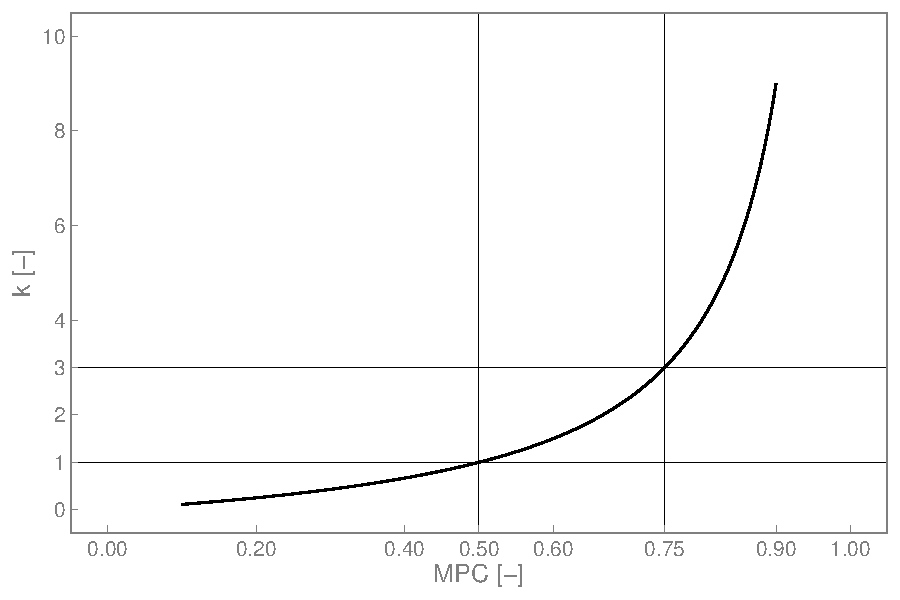
\includegraphics[width=\maxwidth]{figure/k_vs_mpc-1} 

}

\caption{The relationship between $\MPC$ and $k$ in Eq.~(\ref{eq:mpc_and_k_converged}).}\label{fig:k_vs_mpc}
\end{figure}

\end{knitrout}




\end{document}
